\documentclass[11pt, a4paper]{article}
\usepackage[utf8]{inputenc}

\usepackage{amsfonts, amssymb, amsmath}
\usepackage{mathtools}

\usepackage{graphicx}

\usepackage{caption}
\usepackage{subcaption}

\usepackage[colorlinks=true, pdfstartview=FitV, linkcolor=blue, citecolor=blue, urlcolor=blue,pagebackref=false]{hyperref}
\usepackage{varioref}
\usepackage{cleveref}

% BIBLIOGRAPHY MANAGEMENT

\usepackage[numbers]{natbib}
\bibliographystyle{acm}

% PAGE DIMENSIONS

\topmargin -0.5in
\textheight 9 in
\oddsidemargin 0.15in
\evensidemargin 0.25in
\textwidth 6.15in
\parskip=5pt
% THEOREM ENVIRONMENTS

\usepackage{amsthm}
\usepackage{thmtools}

\declaretheorem[numberwithin=section]{theorem}
\declaretheorem[sibling=theorem]{lemma}
\declaretheorem[sibling=theorem]{corollary}
\declaretheorem[sibling=theorem]{proposition}
\declaretheorem[sibling=theorem]{remark}
\declaretheorem[sibling=theorem]{definition}

% COMMENT ENVIRONMENTS

\usepackage{xcolor}
\definecolor{darkred}{rgb}{0.9,0.1,0.1}
\newcommand\comment[1]{\marginpar{\raggedright\scriptsize{\textcolor{darkred}{#1}}}}
\newcommand\myworries[1]{\textcolor{red}{[#1]}}

%%%%%%%%%% ABBREVIATIONS

% BLACKBOARD BOLD

\def \C {{\mathbb C}}
\def \D {{\mathbb D}}
\def \E {{\mathbb E}}
\def \N {{\mathbb N}}
\def \P {{\mathbb P}}
\def \Q {{\mathbb Q}}
\def \R {{\mathbb R}}
\def \Z {{\mathbb Z}}
\def \T {{\mathbb T}}
\def \I {{\mathbb I}}
\def \T {{\mathbb T}}

% MATHCAL

\def \cA {{\mathcal A}}
\def \cC {{\mathcal C}}
\def \cD {{\mathcal D}}
\def \cE {{\mathcal E}}
\def \cF {{\mathcal F}}
\def \cG {{\mathcal G}}
\def \cH {{\mathcal H}}
\def \cI {{\mathcal I}}
\def \cJ {{\mathcal J}}
\def \cK {{\mathcal K}}
\def \cL {{\mathcal L}}
\def \cM {{\mathcal M}}
\def \cN {{\mathcal N}}
\def \cO {{\mathcal O}}
\def \cP {{\mathcal P}}
\def \cQ {{\mathcal Q}}
\def \cR {{\mathcal R}}
\def \cS {{\mathcal S}}
\def \cT {{\mathcal T}}

% VECTORS

\def \vD {{\mathbf D}}
\def \vX {{\mathbf X}}
\def \vZ {{\mathbf Z}}
\def \va {{\mathbf a}}
\def \vc {{\mathbf c}}
\def \vd {{\mathbf d}}
\def \vk {{\mathbf k}}
\def \vs {{\mathbf s}}
\def \vu {{\mathbf u}}
\def \vx {{\mathbf x}}
\def \vy {{\mathbf y}}

% MAKING SUBSET AND SUPSET BY DEFAULT SUBSETEQ AND SUPSETEQ

\def \subset {\subseteq}
\def \supset {\supseteq}

% PAIRED DELIMITERS

\DeclarePairedDelimiter{\abs}{\lvert}{\rvert}
\DeclarePairedDelimiter{\norm}{\lVert}{\rVert}
\DeclarePairedDelimiter{\floor}{\lfloor}{\rfloor}

% MATH OPERATORS

\DeclareMathOperator{\var}{Var}
\DeclareMathOperator{\cov}{Cov}

% MISC SYMBOLS

\def\one{\rlap{\mbox{\small\rm 1}}\kern.15em 1} % indicator function

% CONVERGENCE
\def \todist {\xrightarrow[]{\text{(d)}}}

% PROJECT SPECIFIC SYMBOLS

\usepackage{stmaryrd} % needed for double square brackets
\DeclarePairedDelimiter{\pathbtw}{\llbracket}{\rrbracket}
\def \littleo {o}
\def \bigo {\mathcal O}
\newcommand \diff[2] {\frac{\text{d}#1}{\text{d}#2}}
\newcommand*\dif{\mathop{}\!\mathrm{d}}
\def \lattice {\Lambda}
\newcommand \vectwo[2] {\begin{pmatrix} #1 \\ #2 \end{pmatrix}}
\def \omegaevent {\mathcal E}
\def \maxeval {{\lambda_{\text{max}}}}
\def \mineval {{\lambda_{\text{min}}}}
\def \centeredX {\hat{\vX}}

%%%%%%%%%%%%%%

\title{Metric space convergence under scaling of the strongly connected components of an uniform directed graph with an i.i.d. degree sequence}
\author{Serte Donderwinkel and Zheneng Xie}
\date{Version: \today}

\begin{document}

\maketitle
\tableofcontents
\section{Introduction}


\subsection{Overview}

Edges in real-world networks are often directed, such as links on the world wide web, ``follows'' on Twitter, financial transactions or disease transmission in a social network. When analysing networks, the first quantity that is often considered is the distribution of the degrees of nodes in the network.  In this paper we will consider sampling an i.i.d.\ sequence of in- and out-degrees, conditional on the total in-degree being equal to the total out-degree. We will then sample a uniform directed graph (digraph) with the given degree sequence. Results on such graphs are a useful benchmark, exposing additional underlying structure of a real-world network compared to a uniformly random graph with its degree sequence.

When considering such models, previous work by \citet{cooperSizeLargestStrongly2004} (which we will discuss in more detail in Section \ref{sec.previouswork}) shows that there exists a phase transition in the strong directed connectivity of the graph. Two vertices are part of the same \emph{strongly connected component} (SCC) if and only if there exists a directed cycle that contains both of them. Above some threshold, there will exist a unique giant SCC that occupies a positive proportion of the vertices whereas, below the threshold no SCC will occupy a positive proportion of the vertices. In Figure \ref{fig.SCCs}, a directed graph and its strongly connected components are depicted. In this paper we will prove the first detailed results about the critical case - specifically, that there exists a sequence of random weighted directed multigraphs that can be understood as the scaling limit of the SCCs when viewed in decreasing order of size.

\subsection{Directed graphs}

\begin{figure}
    \centering
    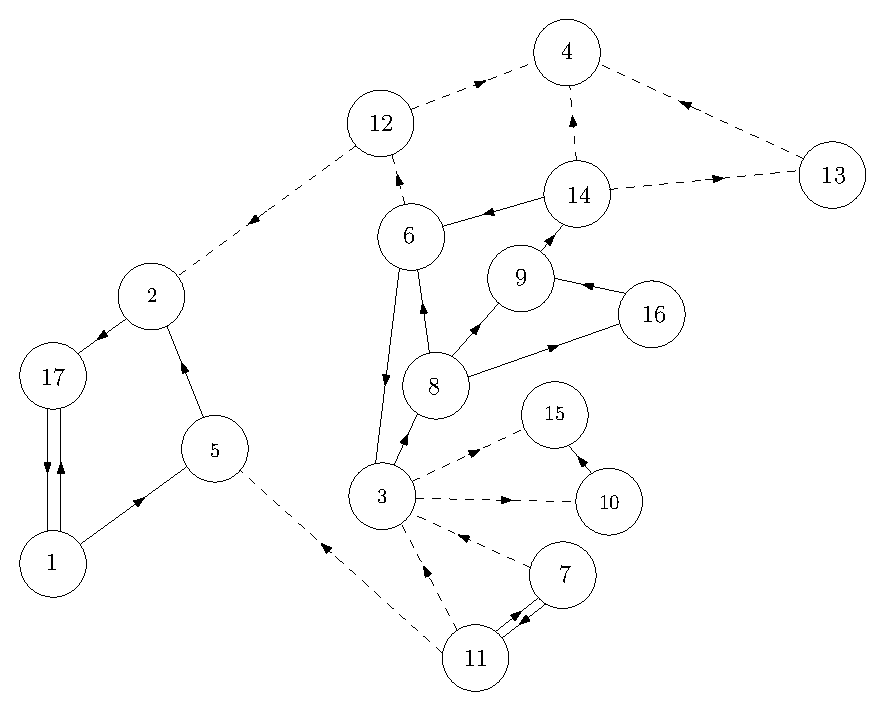
\includegraphics[scale=0.6]{Content/Pictures/Fig1.eps}
    \caption{A directed graph on [17]. The strongly connected components have vertex sets $\{1,2,5,17\}$, $\{3,6,8,9,14,16\}$, $\{7,11\}$, $\{4\}$, $\{10\}$, $\{12\}$, $\{13\}$, and $\{15\}$. Edges that are not part of an SCC are depicted as dashed arrows. Taken from \cite{goldschmidtScalingLimitCritical2019} with permission of the authors.}
    \label{fig.SCCs}
\end{figure}

There are two notions of connectivity when working with a directed graph: weak and strong connectivity. We will be working with the strong notation. We say a vertex $v$ leads to a vertex $w$, written $v \rightarrow w$, if there exists a directed path from $v$ to $w$ in the graph. We say $v$ is \emph{strongly connected to $w$}, written $v \leftrightarrow w$, if $v$ leads to $w$ and $w$ leads to $v$. By convention, $v$ leads to itself. A graph is \emph{strongly connected} if all pairs of vertices in the graph are strongly connected. The relation $v \leftrightarrow w$ is an equivalence relation; the digraphs induced by the equivalence classes of $\leftrightarrow$ are referred to as the \emph{strongly connected components} (SCCs). For each vertex $v$ in a directed graph $\vec{G}$, we will use the notation $d^-(v)$ for the in-degree of $v$ and $d^+(v)$ for the out-degree of $v$. Moreover, a directed edge $(v,w)$ has \emph{tail} $v$ and \emph{head} $w$ (see Figure \ref{fig.tailhead}).
\begin{figure}
    \centering
    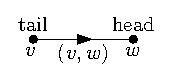
\includegraphics{Content/Pictures/Fig2.eps}
    \caption{An edge $(v,w)$ will be depicted as an arrow from $v$ to $w$.}\label{fig.tailhead}
\end{figure}


\subsection{Description of the model}

\label{subsec:model-description}

First consider a deterministic degree sequence $\vd_1, \ldots, \vd_n$ where $\vd_i = (d_i^-, d_i^+)\in \N \times \N$ for $i = 1, \ldots, n$. We say a directed graph with vertex set $[n]$, where $[n] = \{1,\dots,n\}$, has degree sequence $\vd_1, \ldots, \vd_n$ if $(d^-(i), d^+(i)) = (d_i^-, d_i^+)$ for $i = 1, \ldots, n$.

In order to sample a uniformly random graph with a given degree sequence, we first consider the \emph{directed configuration model} introduced by \citet{cooperSizeLargestStrongly2004}. Take $n$ vertices $v_1, \ldots, v_n$ such that $v_i$ has $d^-_i$ in-half-edges and $d^+_i$ out-half-edges. Then construct a multigraph by choosing a uniformly random pairing of the in-half-edges with the out-half-edges. \citet[Sec.\ 2.1]{cooperSizeLargestStrongly2004} proved that if we condition on the resulting multigraph being simple, we obtain a uniformly chosen random digraph with the given degree sequence.

In this paper we will consider the case where the degree sequence  consists of $n$ i.i.d.\ random variables conditioned on the total in-degree being equal to the total out-degree. Let $\nu$ be a distribution on $\N \times \N$, and let $\vD_1, \ldots, \vD_n$ be a sequence of i.i.d.\ random variables with distribution $\nu$. We condition on the event
\begin{equation*}
    \left\{ \textstyle \sum_{i=1}^n D_i^- = \sum_{i=1}^n D_i^+ \right\},
\end{equation*}
observing that this is an asymptotically singular event as $n\to\infty$. Let $\vec{G}_n(\nu)$ be a digraph chosen uniformly at random from all digraphs with degree sequence $\vD_1, \ldots, \vD_n$. We are interested in the limit under rescaling of the SCCs of $\vec{G}_n(\nu)$ as $n\to \infty$.

Suppose $(D^-, D^+)$ has law $\nu$. We will require the following assumptions to hold:
\begin{enumerate}
    % \item $\E[(D^-) + D^+)^3] < \infty$,
    \item $\E[(D^-)^i(D^+)^j]< \infty$ for $1 \leq i+j\leq 3$, $(i, j) = (1, 3)$ and $(i, j) = (3, 1)$.
    \item $\E[D^-] = \E[D^+]$.
    \item $D^- - D^+$ is strongly aperiodic. This means that for all $p > 1$, there does not exist $k \in \Z$ such that 
    \begin{equation*}
        \P(D^- - D^+ \in k + p\Z) = 1.
    \end{equation*}
    \item $\E[D^-D^+] = \E[D^{\pm}]$.
\end{enumerate}

The first condition is required to ensure that the steps of a random walk used in the proof have finite variance, so that the random walk will convergence under rescaling to a Brownian motion. It also ensures similar regularity of other random variables that we use to encode the directed graph. (We discuss relaxing the moment conditions in Subsection \ref{subsec.openproblems}.)

The second and third conditions make sure the event $\{\sum_{i=1}^n D^-_i = \sum_{i=1}^n D^+_i\}$ is well-behaved. The second condition ensures that it is not a large deviation event. Using a result from \citet[Page 42, P1]{spitzerPrinciplesRandomWalk1964}, the third condition ensures that the event has positive probability for all sufficiently large $n \geq 1$. This condition can be relaxed to assuming that $D^- - D^+$ is non-constant by taking limits for $n \in p \N$ rather than $n \in \N$ where $p$ is the periodicity of $D^- - D^+$. However, for simplicity of presentation, we will keep it as an assumption.

The fourth assumption is the criticality condition. To understand how this arises, consider the directed configuration model and let $(V_n, W_n)$ be a uniformly chosen edge. For now, ignore the conditioning on the total in- and out-degrees being equal. We consider the distribution of the in- and out-degree of $W_n$. Because the degree sequence is an i.i.d.\ sequence, $W_n$ is equally likely to be any vertex $i$. Thus for any $\vk = (k^-, k^+)$,
\begin{align*}
    \P(d^-(W_n) = k^-, d^+(W_n) = k^+)
    &= n \P(W_n = 1, \vD_1 = \vk) \\
    &= n \E[\P(W_n = 1 \mid \vD_1 = \vk, \vD_2, \ldots, \vD_n)] \P(\vD_1 = \vk)
\end{align*}
Conditionally on the degree sequence, we have that $W_n = i$ with probability proportional to $D^-_i$ since we used an uniform pairing of the in- and out-half-edges. Therefore
\begin{align*}
    \P(W_n = 1 \mid \vD_1 = \vk, \vD_2, \ldots, \vD_n)
    &= \frac{k^-}{k^- + \sum_{i=2}^n D_i^-}.
\end{align*}
Thus
\begin{equation*}
    \P(d^-(W_n) = k^-, d^+(W_n) = k^+) = \E\left[ 
        \frac{k^-}{\frac{1}{n}\left( k^- + \sum_{i=2}^n D_i^- \right)}
    \right]
    \P \left[ D^- = k^-, D^+ = k^+ \right].
\end{equation*}
Using the law of large numbers, the above will converge to
\begin{equation*}
    \frac{k^-}{\E[D^-]} \P\left[ D^- = k^-, D^+ = k^+ \right].
\end{equation*}
Let $(Z^-, Z^+)$ be such that $P(Z^- = k^-, Z^+ = k^+)$ is given by the above expression. We say $(Z^-, Z^+)$ has the law of the \emph{degree distribution size-biased by in-degree}. For large $n$, any other fixed out-edge of $W_n$ is then also distributed approximately like a uniformly chosen edge (here we are ignoring the fact that we have already sampled an edge) since we chose the in- and out-edge pairing uniformly at random. Therefore the out-degree of the head will have approximately the same distribution as $Z^+$. Thus if we were to look at the graph of all vertices leading from $W_n$, it would look approximately like a Bienaymé tree\footnote{For $\mu$ a probability distribution on $\N$, a Bienaymé tree with offspring distribution $\mu$ is the family tree of a branching process with offspring distribution $\mu$. Bienaymé trees are often referred to as Galton-Watson trees, but we decide to follow the name change suggested by \citet{addarioberry2021universal}.} with offspring distribution $Z^+$. It is well known that such trees exhibit critical behaviour in whether or not the tree is finite at $\E[Z^+] = 1$. This is equivalent to assuming $\E[D^-D^+] = E[D^-]$.

\citet{cooperSizeLargestStrongly2004} studied this phase transition for a deterministic degree sequence $\vd_1, \ldots, \vd_n$. They defined the parameter
\begin{equation*}
    d = \frac{\sum_{i=1}^n d_i^+ d_i^-}{\sum_{i=1}^n d_i^-}
\end{equation*}
which is a counterpart of $\E[Z^-]$ for deterministic degree sequences. They then showed that, under additional assumptions, there exists a phase transition for the existence of a giant SCC depending on whether $d$ is strictly greater than or less than 1. Our work in this paper shows our corresponding condition, $\E[Z^-] = 1$, is also the correct criticality condition to take for i.i.d.\ random degree sequences.

We define the following parameters that will determine the behaviour of the SCCs in the limit.
\begin{enumerate}
    \item $\mu:=\E[D^-]=\E[D^+]=\E[D^-D^+]$
    \item $\nu_-:= \E[Z^-] - 1 = \frac{\E[(D^-)^2]-\mu}{\mu}$ 
    \item $\sigma_-^2 := \var(Z^-) = \frac{\mu\E[(D^-)^3]-\E[(D^-)^2]^2}{\mu^2}$ 
    \item $\sigma_+^2 := \var(Z^+) = \frac{\E[D^-(D^+)^2]-\mu}{\mu}$ 
    \item $\sigma_{-+} := \cov(Z^-, Z^+) = \frac{\E[(D^-)^2D^+]-\E[(D^-)^2]}{\mu}$ 
\end{enumerate}
% \begin{remark}
% Conditions \ref{cond.beta} and \ref{cond.gamma} ensure that the Central Limit Theorem applies to the fluctuations of the first explored in-degrees around their mean. Condition \ref{cond.critical} ensures that the branching process corresponding to the depth-first exploration (i.e. the exploration of the out-components) is critical. Condition \ref{cond.rho} ensures that this branching process has Brownian scaling. Condition \ref{cond.tau} ensures that the covariance of the in- and out-degrees that are discovered first is finite. Condition \ref{cond.iota} ensures that the strongly connected components are $3$-regular. 
% \end{remark}
\subsection{Metric directed multigraphs and kernels}\label{subsec.mdmkernels}

\begin{figure}[htbp]
    \centering

    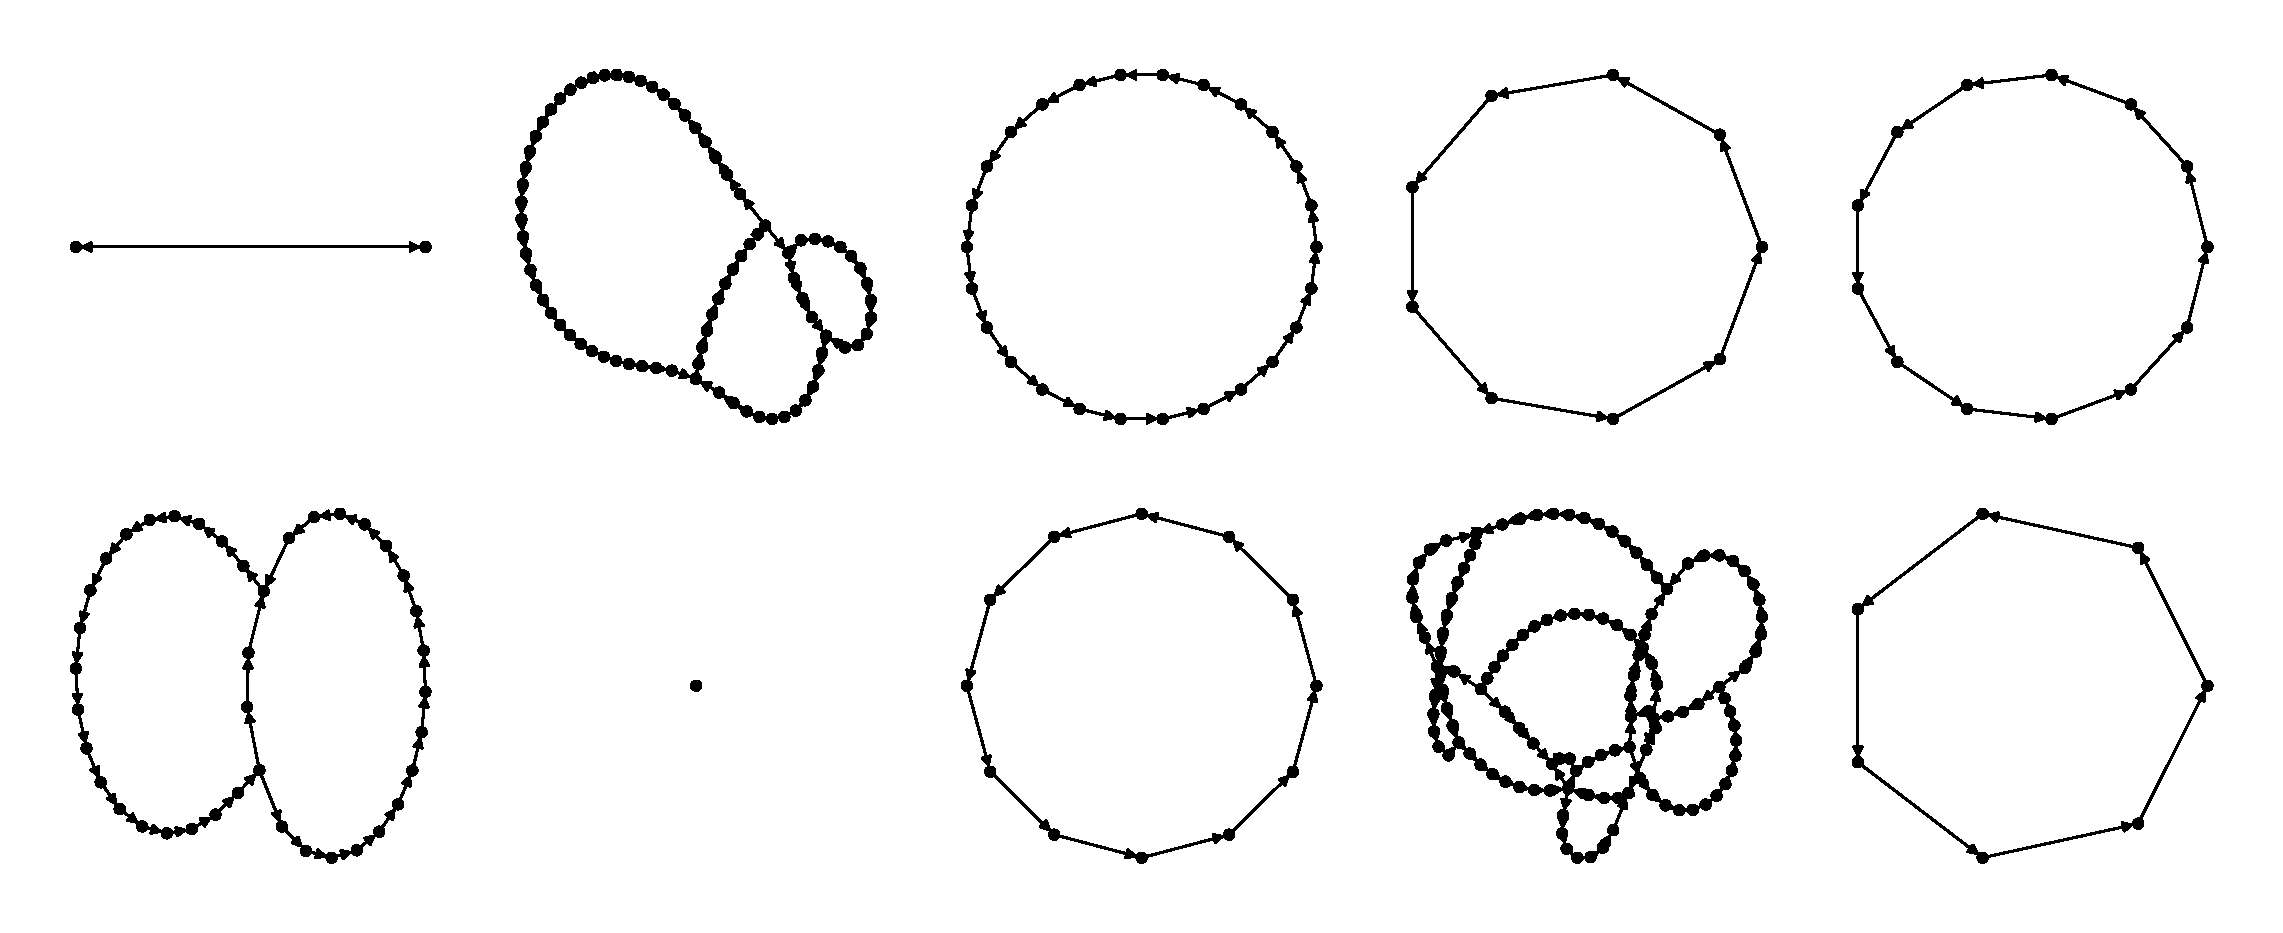
\includegraphics[width=\textwidth]{Content/Pictures/Fig3.eps}
    
    \caption{The largest SCC from samples of a directed configuration model with independent $\text{Poisson(1)}$ in- and out-degrees}
    \label{fig:largest-sccs}
\end{figure}

Figure \ref{fig:largest-sccs} shows the largest SCC from samples of a directed configuration model. As can be seen, while the lengths of paths in the SCC are long, the actual structure of the SCC is often quite simple. Previous work by \citet{goldschmidtScalingLimitCritical2019} shows that this is true for the \emph{directed Erdős--Rényi model} in the \emph{critical window}. The \emph{directed Erd\H{o}s--Rényi model} on $n$ vertices with parameter $p$, denoted by $\vec{G}(n,p)$, is a random digraph with vertex set $[n]$ in which each of the $n(n-1)$ possible directed edges is included with probability $p$ independently. The cases $p=(1+\lambda n^{-1/3})/n$ for $\lambda\in\R$ are referred to as \emph{the critical window}, and the case $p=1/n$ is called \emph{criticality}. In \cite{goldschmidtScalingLimitCritical2019}, it was shown that, for the directed Erdős--Rényi model in the critical window, while the lengths of paths in the SCCs scale like $n^{1/3}$, the combinatorial structure of the SCCs remains finite. The same turns out to be true in our setting.

This idea was formalised in \cite{goldschmidtScalingLimitCritical2019}, and we will use the same formalism in this work. We will first introduce \emph{metric directed multigraphs} (MDMs). These are simply weighted directed multigraphs, but in our context it is more appropriate to think of the weights as lengths, which motivates the change in naming. Formally, a \emph{directed multigraph} is a tuple $(V, E, r)$ where
\begin{enumerate}
    \item $V$ is a set of \emph{vertices},
    \item $E$ is a set of \emph{edges}, and
    \item $r: E \to V \times V$ is a function mapping each edge to its \emph{head} and \emph{tail}; associated with $r$ are two functions $r_1: E \to V$ and $r_2: E \to V$ such that
\begin{equation*}
    r(e) = (r_1(e), r_2(e))
\end{equation*}
for all $e \in E$. $r_1(e)$ is the tail of the edge $e$ and $r_2(e)$ is the head of the edge $e$.
\end{enumerate}
 Then a \emph{metric directed multigraph (MDM)} is a tuple $M = (V, E, r, l)$ where $(V, E, r)$ is a directed multigraph and $l:E \to [0, \infty)$. Let $\zeroloop$ denote the MDM consisting of a single vertex with a self-loop of length 0.

An \emph{isomorphism} between two MDMs $M = (V, E, r, l)$ and $M' = (V', E', r', l')$ is a pair of functions $(i_V, i_E)$ where $i_V: V \to V'$ and $i_E: E \to E'$ are bijections satisfying the relation
\begin{equation*}
    r'(i_E(e)) = (i_V(r_1(e)), i_V(r_2(e)))
\end{equation*}
for all $e \in E$. We say two MDMs are \emph{isomorphic} if there exists an isomorphism between them. In other words, isomorphic MDMs have the same graph structures for their underlying directed multigraphs up to a relabelling of the edges and vertices. Write $\iso(M, M')$ for the set of all isomorphisms between $M$ and $M'$.

We now define a distance $\distmdm$ between two MDMs $M$ and $M'$.  Any isomorphism between $M$ and $M'$ gives a correspondence between the edges of $M$ and the edges of $M'$. We can then take an $\ell_{\infty}$ distance between the lengths of the edges and finally take the isomorphism which minimizes this distance. If $M$ and $M'$ are not isomorphic, we set the distance to be infinite. Formally,
\begin{equation*}
    \distmdm(M, M') = \begin{cases}
        \inf_{(i_V, i_E) \in \iso(M, M')} \sup_{e \in E} \abs{l(e) - l'(i_E(e))} & \text{if $M$ and $M'$ are isomorphic,} \\
        \infty & \text{otherwise.}
    \end{cases}
\end{equation*}
Consider an MDM $M$ and a vertex $w \in M$ with in-degree 1 and out-degree 1 which is not a self-loop. Let $u$ and $v$ be the unique in-neighbour and out-neighbour of $w$ respectively. The MDM obtained by \emph{smoothing} $w$ is obtained by deleting the edges $e_1$ and $e_2$ such that $r(e_1) = (u, w)$ and $r(e_2) = (w, v)$, then adding an edge $e$ such that $r(e) = (u, v)$ and assigning it length $l(e) = l(e_1) + l(e_2)$. This is illustrated in Figure \ref{fig:smoothing}. 
\begin{figure}[htbp]
    \centering
    \begin{subfigure}[htbp]{0.45\textwidth}
        \centering
        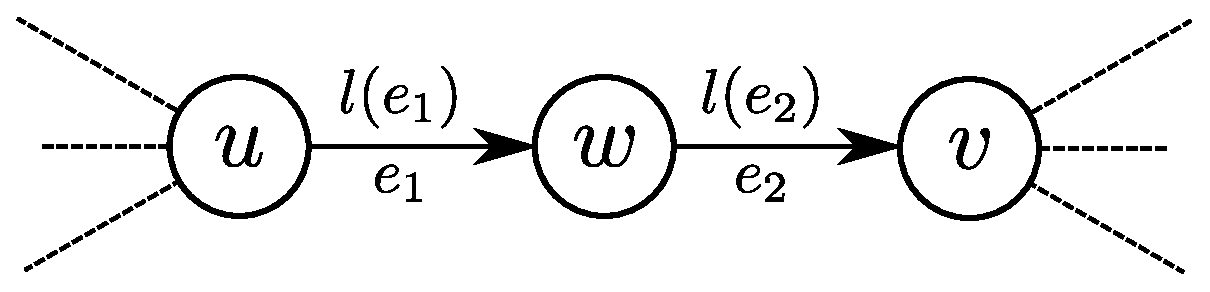
\includegraphics[width=0.95\textwidth]{Content/Pictures/Fig4a.eps}
        \caption{The graph before smoothing $w$}
    \end{subfigure}
    \hfill
    \begin{subfigure}[htbp]{0.45\textwidth}
        \centering
        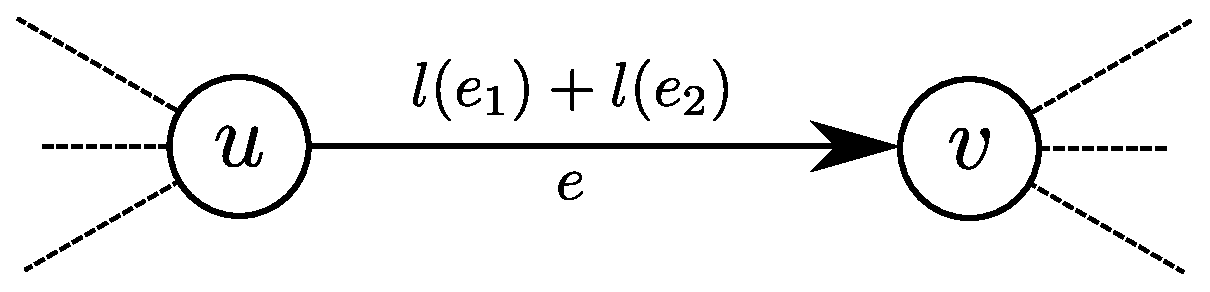
\includegraphics[width=0.95\textwidth]{Content/Pictures/Fig4b.eps}
        \caption{The graph after smoothing $w$}
    \end{subfigure}
    \caption{Smoothing a vertex $w$}
    \label{fig:smoothing}
\end{figure}

Then the kernel of a digraph $\vec{G}$ is obtained by doing the following:
\begin{enumerate}
    \item Assign length $1$ to each edge.
    \item Iteratively smooth vertices with in-degree 1 and out-degree 1 that are not self-loops until there are none remaining.
    \item Replace all singletons by $\zeroloop$.
\end{enumerate}
An example is shown in Figure \ref{fig:kernel}.
\begin{figure}[htbp]
    \centering
    \begin{subfigure}[htbp]{0.45\textwidth}
        \centering
        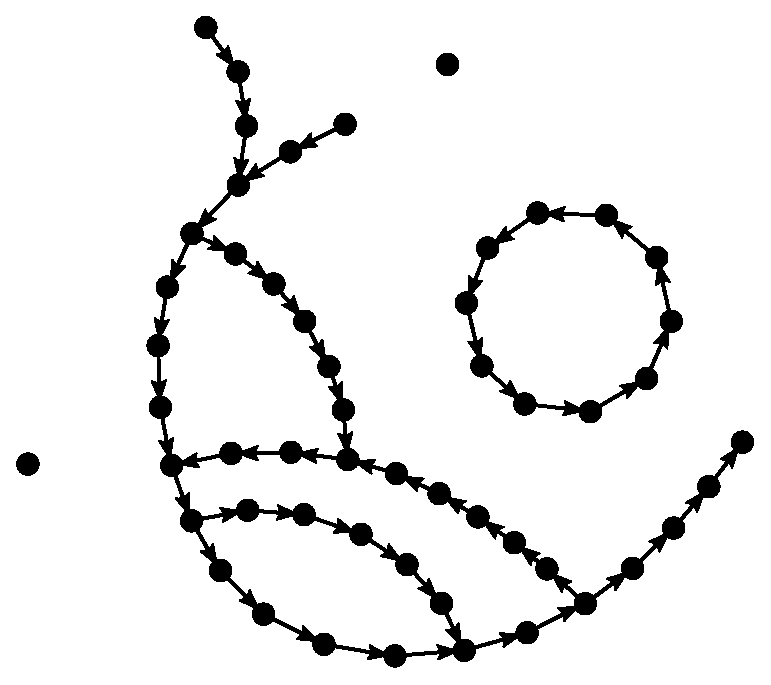
\includegraphics[width=0.90\textwidth]{Content/Pictures/Fig5a.eps}
        \caption{$\vec{G}$}
    \end{subfigure}
    \hfill
    \begin{subfigure}[htbp]{0.45\textwidth}
        \centering
        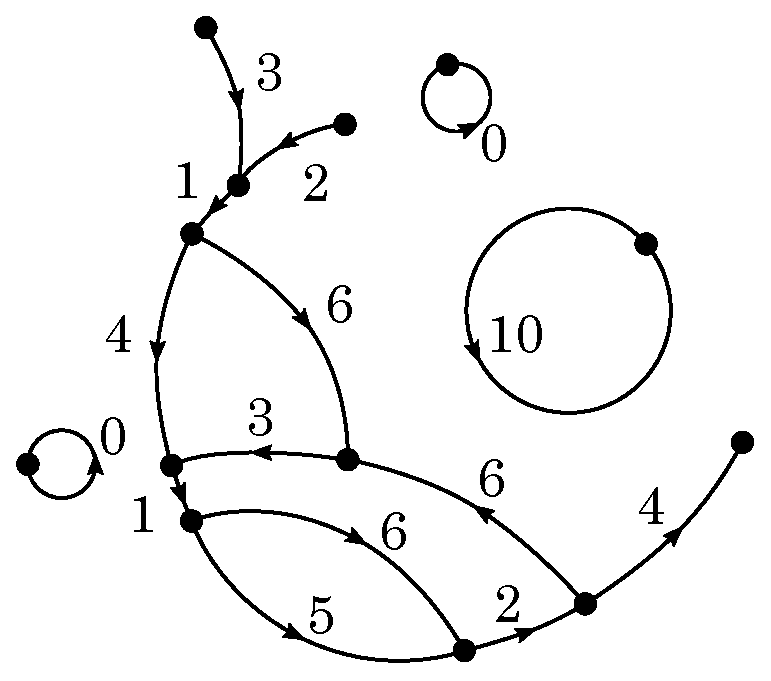
\includegraphics[width=0.90\textwidth]{Content/Pictures/Fig5b.eps}
        \caption{Kernel of $\vec{G}$}
    \end{subfigure}
    \caption{An example of a digraph $\vec{G}$ and its kernel. The numbers indicate the edge lengths.}
    \label{fig:kernel}
\end{figure}



\subsection{Our results}

For $M$ an MDM and $c\in (0,\infty)$, let $cM$ be equal to $M$ with all lengths multiplied by $c$. Let $C_i(n)$ for $i\geq 1$ be the kernels of the SCCs of $\vec{G}_n(\nu)$, listed in decreasing order of number of edges, breaking ties arbitrarily. Complete the list with an infinite repeat of $\zeroloop$. Then, our main theorem is as follows.
\begin{theorem}\label{thm.main}
There exists a sequence $\cC=(\cC_i,i\in \N)$ of random strongly connected MDMs such that 
$$\left(n^{-1/3}C_i(n),i\in \N\right)\todist\left(\cC_i,i\in \N\right)$$
as $n\to \infty$, with respect to the product $d_{\vec{\cG}}$-topology. The law of $\cC=(\cC_i,i\in \N)$ depends only on the parameters $\mu$, $\sigma_+$, and $(\sigma_{-+}+\nu_-)/\mu$. Further, for each $i\geq 1$, $\cC_i$ is either $3$-regular or a loop.
\end{theorem}
We will describe the limit object and some of its further properties in Subsection \ref{subsec.limitobject}.

The law of the limit object places some particular cases of our model in the universality class of the directed Erd\H{o}s--Rényi model as studied by \citet{goldschmidtScalingLimitCritical2019}. This is the content of the following corollary. Note however that their result holds in a stronger topology: they use an $\ell_1$-like topology on the space of sequences of MDMs, whereas we show our result in the product topology. Due to this, it is important in their paper to consider singletons as loops of length zero. For any fixed $k$, the $k$th largest SCC will not be a singleton with high probability as $n \to \infty$. Therefore, no component of our limiting object will be a singleton. Thus they need to pad their SCCs by $\zeroloop$ and consider the kernel of singletons to be $\zeroloop$, to prevent the $\ell_1$-distance, as defined by $d_{\vec{G}}$, between $\left(n^{-1/3}C_i(n),i\in \N\right)$ and $\left(\cC_i,i\in \N\right)$ being infinite. We follow the same convention.

\begin{theorem}\label{cor.erdosrenyi}
Consider $\vec{G}_n(\nu)$, with $\nu$ such that $$\mu=\sigma_+=\sigma_{-+}+\nu_-=1.$$ 
Let $(C^\nu_i(n), i\geq 1)$ be the kernels of the SCCs of $\vec{G}_n(\nu)$. Furthermore, let $(C^{ER}_i(n), i\geq 1)$ be the kernels of the SCCs of $\vec{G}(n,1/n)$. Then, $\left(n^{-1/3}C^\nu_i(n),i\in \N\right)$ and 
$\left(n^{-1/3}C^{ER}_i(n),i\in \N\right)$ have the same limit in distribution in the product-$d_{\vec{\cG}}$-topology as $n\to \infty$. 
\end{theorem}
Note that the condition in Corollary \ref{cor.erdosrenyi} is satisfied by $\nu(k^-,k^+)=\nu_1(k^-)\nu_2(k^+)$, with $\nu_1$ and $\nu_2$ the law of a $\operatorname{Poisson}(1)$ random variable.

Moreover, Theorem \ref{thm.main} has the following trivial corollaries, which were previously unknown. 
\begin{corollary}\label{cor.componentsizes}
Let $E^i_n$ and $V^i_n$ be the number of edges and vertices in $C_i(n)$ respectively, both appended with infinite repeats of $0$. Then there exists a random sequence $(E_i,i\in \N)\in \R_+^\infty$, such that
$$\left(n^{-1/3}E^n_i,n^{-1/3}V^n_i, i\in \N\right)\todist\left(E_i,E_i,i\in \N\right)$$
as $n\to \infty$ in the product topology on $(\R^2)^\infty$. 
\end{corollary}
In particular, note that, in the above corollary, the number of vertices and number of edges have the exact same scaling limit.
\begin{corollary}\label{cor.diameter}
For $v,w\in \vec{G}_n(\nu)$ such that $v\to w$, let $d(v,w)$ denote the length of the shortest directed path from $v$ to $w$, and let $$\operatorname{Diam}\left(\vec{G}_n(\nu)\right)=\max_{v,w\in V}\{d(v,w):v\to w\}$$ be the \emph{diameter} of $\vec{G}_n(\nu)$. Then, for any $\epsilon>0$, there is a $\delta>0$ such that $$\P\left( n^{-1/3}\operatorname{Diam}\left(\vec{G}_n(\nu)\right)>\delta\right)>1-\epsilon$$ for all $n$ large enough. Equivalently, $\operatorname{Diam}\left( \vec{G}_n(\nu) \right) = \Omega_p(n^{1/3})$.
\end{corollary}


\subsection{Previous work}\label{sec.previouswork}
The configuration model was introduced by \citet{Bollobas1980} to sample a uniformly random undirected graph with a given degree sequence. (For a discussion of the configuration model and proofs of standard results, we refer the reader to \cite[Chapter 7]{hofstadRandomGraphsComplex2017}.)

Most results on the configuration model are proved for models with a deterministic degree sequence. The phase transition for the undirected setting was shown in \cite{molloyCriticalPointRandom1995, Molloy1998, Janson2009}. The law of component sizes at criticality and in the critical window were obtained by \citet{Riordan2012} under the assumption that the degrees are bounded. Dhara, van der Hofstad, van Leeuwaarden and Sen showed convergence of the size and surplus edges in the critical window with a finite third moment \cite{Dhara2017} and in the heavy-tailed regime \cite{Dhara2020}.  Bhamidi, Dhara, van der Hofstad and Sen obtained metric space convergence in the critical window in \cite{Bhamidi2020}, a result that the authors later improved to a stronger topology in \cite{Bhamidi2020Glmb}. 

Configuration models with a random degree sequence are considered in \cite{josephComponentSizesCritical2014}, \cite{conchon--kerjanStableGraphMetric2021}, and \cite{Donderwinkel2021heightprocess}. \citet{josephComponentSizesCritical2014} showed convergence of the component sizes and surpluses of the large components under rescaling at criticality, both for degree distributions with finite third moments and for the heavy-tailed regime. \citet{conchon--kerjanStableGraphMetric2020} show Gromov-Hausdorff-Prokhorov convergence of the rescaled components ordered by decreasing size at criticality in these two regimes. The results in \cite{conchon--kerjanStableGraphMetric2020} in the heavy-tailed regime are extended to the critical window by the first author in \cite{Donderwinkel2021heightprocess}. Our techniques are closely related to the techniques introduced in \cite{conchon--kerjanStableGraphMetric2020}. 

Some results have been obtained for other directed graph models. \citet{caoConnectivityGeneralClass2019} consider a class of inhomogeneous directed random graphs. Their results include a phase transition for the existence of a giant SCC. This is a generalisation of work by Bloznelis, Götze and Jaworski in \cite{Bloznelis2012}, in which a smaller class of inhomogeneous directed graphs is considered. Samorodnitsky, Resnick, Towsley, Davis, Willis and Wan \cite{Samorodnitsky2016} studied the tails of the degree distribution in the directed preferential attachment model. \citet{goldschmidtScalingLimitCritical2019} studied the directed Erd\H{o}s-R\'enyi model, and were the first to obtain metric space convergence of the SCCs of a directed graph. Our methods build on their techniques.

The directed configuration model was first considered by \citet{cooperSizeLargestStrongly2004}. They consider a deterministic degree sequence under a number of conditions. As discussed previously in \cref{subsec:model-description}, a phase transition for the SCCs occurs when a parameter $d=1$. They show that for $d<1$, with high probability, all SCCs contain $O(\Delta\log(n))$ vertices, for $\Delta$ the maximal degree. On the other hand, for $d>1$, there is a unique SCC that contains a positive proportion of the vertices and edges. Their conditions are restrictive, and include finite second moments for both the in- and out-degree of a uniformly chosen vertex, and a bound of size $n^{1/12}/\log(n)$ on the largest degree. Their proofs are based on an algorithm to explore the directed graph. The condition on the largest degree was later relaxed to $O(n^{1/4})$ by \citet{Graf2016}. These results are in contrast with the critical case, with Corollary \ref{cor.componentsizes}, which says that in our set-up the number of vertices and edges in the largest strongly connected components are $\Theta(n^{1/3})$ in probability.

Recently, Cai and Perarnau have obtained a number of results on the directed configuration model with deterministic degrees. In \cite{caiDiameterDirectedConfiguration2020}, they show, under first and second moment conditions of the degree of a uniformly picked vertex, for $d\neq 1$ (i.e. not at criticality), that the diameter of the model on $n$ vertices, rescaled by $\log(n)$ converges to a constant that they identify. This is in contrast with Corollary \ref{cor.diameter}, which says that in our set-up the diameter is $\Omega(n^{1/3})$ in probability at criticality. Then, in \cite{caiGiantComponentDirected2020}, they show a law of large numbers for the number of vertices and edges in the largest SCC, under slightly stronger moment conditions, and again away from the critical point. In \cite{cai2021rw}, they study the behaviour of a random walk on a directed configuration model.
 
A necessary and sufficient condition for the existence of a giant weakly connected component for the directed configuration model with a deterministic degree sequence is discussed in the physics literature by \citet{Kryven2016}. He also studies the distribution of the in- and out-components in \cite{Kryven2017}.

The directed configuration model with random in- and out-degrees is also considered by \citet{chenDirectedRandomGraphs2013} although, importantly, they do not allow for the in- and out-degree of a vertex to be dependent. The authors consider a model in which the in- and out-degrees are two independent sequences of i.i.d.\ random variables drawn from different probability distributions. They propose an algorithm to sample degree sequences that correspond to a simple graph and show the limiting distribution of the degrees generated by this algorithm. 



\subsection{Proof outline}\label{sec:proofoutline}

\def \exploredvertices {\mathcal V}
\def \explorededges {\mathcal E}
\def \forest {F}
\def \edgestack {\mathcal Q}

The techniques we will use to investigate the graph model are a combination of the techniques introduced by Conchon-Kerjan and Goldschmidt in \cite{conchon--kerjanStableGraphMetric2020} and the strategy of Goldschmidt and Stephenson in \cite{goldschmidtScalingLimitCritical2019}, adapted to our set-up. The former work finds the scaling limit of an undirected uniform graph with i.i.d.\ degrees at criticality, and the latter finds the scaling limit of the SCCs of a directed Erd\H{o}s-Rényi graph at criticality. 

Our techniques use height processes and \L ukasiewicz paths, which are standard objects used to encode trees and forests (see for instance \cite[Chapter 0]{AST_2002__281__R1_0}). We will introduce these here. Let $T=(V,E,\rho)$ be an ordered rooted finite tree with vertex set $V$, edge set $E$ and root vertex $\rho$; say $|V|=n$. Let $v_0,\dots,v_{n-1}$ denote the vertices of the tree visited in depth-first order, so that $v_0=\rho$. We can view $T$ as a metric space by regarding all edges as line segments of length $1$ that are connected via the vertices. The distance $d_T$ between points $a_1$ and $a_2$ on line segments $l_1$ and $l_2$ respectively is then defined as the length of the unique non-self-intersecting path between $a_1$ and $a_2$ that traverses the line segments of the tree. Denote $(T,d_T)$ by $\mathrm{T}$.\\
We will define the height process and \L ukasiewicz path of $\mathrm{T}$. Both of these functions uniquely characterize $\mathrm{T}$. The height process of $\mathrm{T}$, referred to as $h$, is defined as $$h(i)=d_T(v_i,v_0),$$ i.e.  for all $i$, $h(i)$ equals the distance from $v_i$ to the root.
Moreover, for all $i=1,\dots,n$, let $y_i$ be the number of children of $v_{i-1}$, and set $y_0=1$. Then, the \L ukasiewicz path of $\mathrm{T}$ is defined by $$s(i)=\sum\limits_{j\leq i} (y_j-1)$$ for $i=0,\dots,n$. Then, $s(i)$ is the total number of younger siblings of $v_i$ and its ancestors.
For a sequence of ordered rooted finite trees, we define its height process by concatenating the height processes of the trees in the sequence. The \L ukasiewicz path is defined similarly. 

We will study the law of the SCCs of a uniform directed graph with degree sequence $(\mathbf{D}_1,\dots,\mathbf{D}_n)$, conditional on $\sum_{i=1}^n D^-_i=\sum_{i=1}^n D^+_i$ by exploring the configuration model in a depth-first manner. This sampling naturally gives rise to a directed subforest of the resulting multigraph, which we call the \emph{out-forest}. The sampling procedure is  described in \cref{alg:edfs}, and is also illustrated in Figure \ref{fig.configuration model}. The definition of the out-forest is illustrated in Figure \ref{fig.configuration modeloutforest}.  

\begin{figure}
    \begin{subfigure}[htbp]{\textwidth}
        \centering
        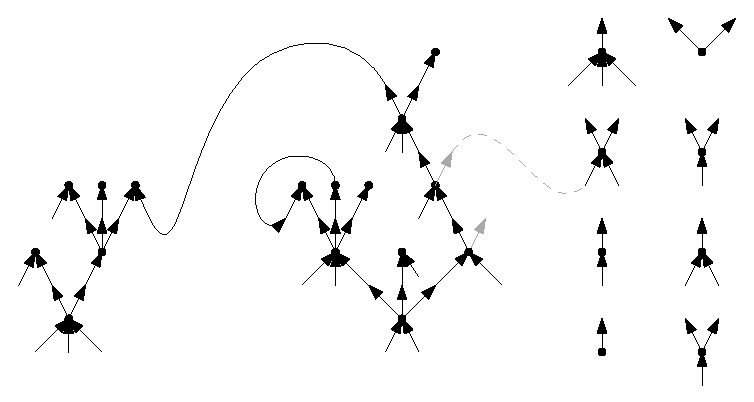
\includegraphics[scale=1]{Content/Pictures/Fig6a.eps}
        \caption{The gray arrows represent unpaired out-half-edges of vertices that have been discovered. One by one, in depth first order, these are paired to a uniform unpaired in-half-edge.}
        \label{fig.configuration model}
    \end{subfigure} \\

    \vspace{2em}

    \begin{subfigure}[htbp]{\textwidth}
        \centering
        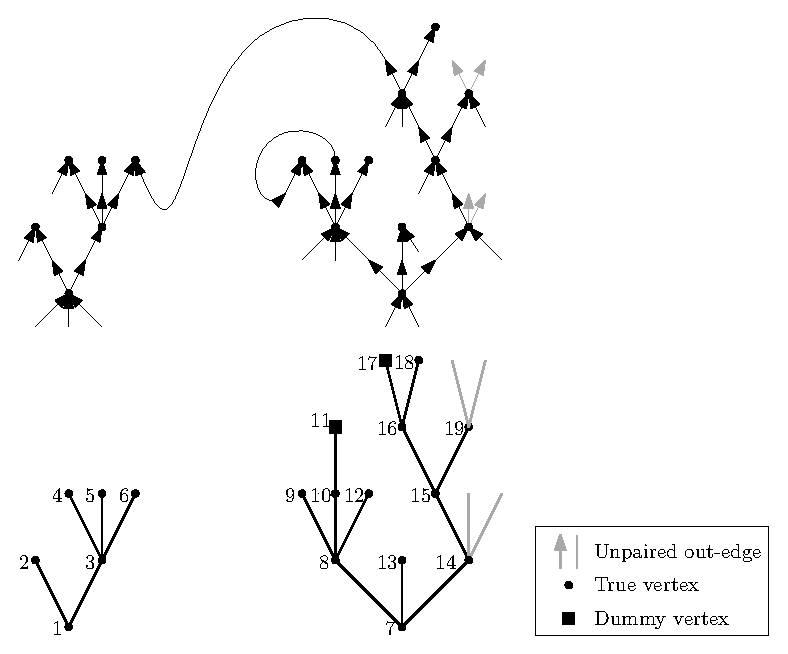
\includegraphics[scale=1]{Content/Pictures/Fig6b.eps}
        \caption{The out-forest is defined based on the exploration of the digraph. For each surplus edge, we add a dummy leaf. The labels of the vertices correspond to the time step in the exploration at which the vertex is added. The gray edges lead to vertices of which we do not know whether it is a dummy vertex, and if not, what its degree is. }
        \label{fig.configuration modeloutforest}
    \end{subfigure}

    \caption{Partial constructions of the configuration model and out-forest}
\end{figure}

% This procedure differs from the exploration used by \citet{goldschmidtScalingLimitCritical2019}.  The eDFS takes as input a directed multigraph and uses a stack (ordered list) of edges. When the stack is empty, we are at the start of a new out-component and pick a new vertex $w$ with probability proportional to its in-degree. Otherwise we remove the last edge $(v, w)$ from the stack. In both cases, if $w$ is not yet in the list of discovered vertices, we add the out-edges from this vertex to the \emph{end} of the stack of edges (this choice is what makes the exploration depth-first) and add $w$ to the list of discovered vertices $\exploredvertices$.  The order in which vertices are added to $\exploredvertices$ is referred to as their \emph{order of discovery}. Note that we will not discover any vertex with in-degree 0. From the perspective of finding the SCCs, this is not a problem since such vertices will form singleton SCC.

The sampling procedure uses a queue of unpaired out-edges (represented by the label of their corresponding vertex). When the queue is empty, we are at the start of a new out-component and pick a new vertex $w$ with probability proportional to its in-degree if there are vertices with positive in-degree remaining. Else, we pick a new vertex uniformly at random. If the queue is not empty, we pair the first out-edge in the queue to a uniform unpaired in-edge and call the corresponding vertex $w$. In both cases, if $w$ is not yet in the list of discovered vertices, we add the out-edges from this vertex to the \emph{front} of the queue of edges (this choice is what makes the exploration depth-first) and add $w$ to the list of discovered vertices. The order in which vertices are added to the list of discovered vertices is referred to as their \emph{order of discovery}. 

This procedure will discover vertices with in-degree 0 last. This is fine since such vertices form singleton SCCs, so we have discovered the non-trivial SCCs first.

\begin{algorithm}[htbp]
    \SetAlgoLined
    \KwData{A set of vertices $V=\{v_1,\dots, v_n\}$ with degree pairs $(d^-(v_1),d^+(v_1)),\dots, (d^-(v_n),d^+(v_n))$ satisfying $\sum d^-(v_i)=\sum d^+(v_i)$}
    $\exploredvertices \leftarrow$ an empty ordered list of vertices \tcp*[f]{the list of discovered vertices}\;
    $\edgestack \leftarrow$ an empty ordered list of vertices \tcp*[f]{the queue}\;
    $(d^-_{\mathrm{unpaired}}(v_1),\dots,d^-_{\mathrm{unpaired}}(v_n))\leftarrow (d^-(v_1),\dots,d^-(v_n))$  \tcp*[f]{the number of unpaired in-edges per vertex}\;
    $k \leftarrow 0$ \tcp*[f]{the index of the current step} \;
    $\hat{s}^- \leftarrow 0$ \tcp*[f]{the number of unpaired in-edges of discovered vertices}\;
    $\hat{s}^+ \leftarrow 1$ \tcp*[f]{the queue size minus the number of explored out-components} \;
    $\forest \leftarrow$ a directed forest with vertices $V$ and no edges
    \tcp*[f]{current out-forest}\;
     $M \leftarrow$ a directed multigraph with vertices $V$ and no edges
    \tcp*[f]{current di-multigraph}\;
    \While(){there exist undiscovered vertices OR $\edgestack$ is non-empty}{
        \eIf(\tcp*[f]{we start a new out-component}){$\edgestack$ is empty}{
            \eIf(){there exist undiscovered vertices with positive in-degree}{
            $w\leftarrow$ a random vertex not in $\exploredvertices$ chosen with prob.\ proportional to $d^-(w)$ \;}
            {$w\leftarrow$ a uniformly random vertex not in $\exploredvertices$}
            $\hat{s}^+\leftarrow \hat{s}^+-1$\tcp*[f]{we have explored a component}\;}{
            $v \leftarrow$ first entry in $\edgestack$ \tcp*[f]{we will pair an unpaired out-edge of $v$}\;
            remove first entry from $\edgestack$ \;
            $\hat{s}^+\leftarrow \hat{s}^+-1$\tcp*[f]{the queue size decreases by $1$}\;
            $w \leftarrow$ a random vertex chosen with prob.\ proportional to $d^-_{\mathrm{unpaired}}(w)$ \;
            add $(v,w)$ to $M$\tcp*[f]{we pair the out-edge of $v$ with a uniform unpaired in-edge}\;
            $d^-_{\mathrm{unpaired}}(w)\leftarrow d^-_{\mathrm{unpaired}}(w)-1$\;
            $\hat{s}^-\leftarrow \hat{s}^--1$\tcp*[f]{we have paired an in-edge}\;
            \eIf(\tcp*[f]{we sampled a surplus edge}){$w\in \exploredvertices$}{
            add a dummy leaf to $F$ and an edge from $v$ to the leaf\;}{
            add $(v,w)$ to $F$\;
            }
        }
        \If(){$w\not\in \exploredvertices$}{
        append $w$ to the end of $\exploredvertices$ \tcp*[f]{vertex $w$ is now discovered}\;
        append $d^+(w)$ repeats of $w$ to the start of $\edgestack$\;
        $\hat{s}^+\leftarrow \hat{s}^++d^+(w)$\tcp*[f]{the queue size has increased}\;
        $\hat{s}^-\leftarrow \hat{s}^-+d^-(w)$\tcp*[f]{the number of unpaired in-edges of discovered vertices has increased}\;
        }
        $k\leftarrow k+1$\;
        $\hat{s}^+_k\leftarrow \hat{s}^+$\;
        $\hat{s}^-_k\leftarrow \hat{s}^-$ \;
        }
    
    
    \caption{The edge depth-first configuration model \label{alg:edfs}}
\end{algorithm}
% \begin{algorithm}[htbp]
%     \SetAlgoLined
%     \KwData{A set of vertices $\{v_1,\dots, v_n\}$ with degree pairs $(d^-(v_1),d^+(v_1)),\dots, (d^-(v_n),d^+(v_n))$ satisfying $\sum d^-(v_i)=\sum d^+(v_i)$}
%     $\exploredvertices \leftarrow$ an empty ordered list of vertices \tcp*[f]{the list of discovered vertices}\;
%     $\edgestack \leftarrow$ an empty ordered list of vertices \tcp*[f]{the queue}\;
%     $(d^-_{\mathrm{unpaired}}(v_1),\dots,d^-_{\mathrm{unpaired}}(v_n))\leftarrow (d^-(v_1),\dots,d^-(v_n))$  \tcp*[f]{\# unpaired in-edges per vertex}\;
%     $\forest \leftarrow$ an empty directed graph
%     \tcp*[f]{the current out-forest}\;
%      $G \leftarrow$ an empty directed graph
%     \tcp*[f]{the current directed-graph}\;
%     \While(){there exist unpaired out-half-edges of vertices with positive in-degree}{
%         \eIf(\tcp*[f]{we are starting a new out-component}){$\edgestack$ is empty}{
%             $w \leftarrow$ a random vertex not in $\exploredvertices$ chosen with prob.\ proportional to $d^-(w)$ \;
%         }(){
%             $v \leftarrow$ last entry in $\edgestack$ \;
%             remove last entry from $\edgestack$ \;
%             $w \leftarrow$ a random vertex chosen with prob.\ proportional to $d^-_{\mathrm{unpaired}}(w)$\;
%         }
%         \eIf(){$w \not \in \exploredvertices$}{
%             append $w$ to $\exploredvertices$ \; 
%             add the vertex $w$ to $\forest$ \;
%             add the vertex $w$ to $M$ \;
%             \If(){$\edgestack$ is non-empty}{
%                 add the edge $(v, w)$ to $\forest$\;
%                 add the edge $(v, w)$ to $M$\;
%             }
%             append $d^+(w)$ repeats of $w$ to the end of $\edgestack$ \;
%         }{
%             add a dummy leaf to $\forest$ and and edge from $v$ to the leaf \tcp*[f]{we have discovered a surplus edge and add a dummy leaf to the forest} \;
%             add the edge $(v, w)$ to $M$\;
%         }
%     }
%     \While(){there exist unpaired out-half-edges}{
%     \eIf(){$\cQ$ is empty}
%     {$w\leftarrow$ a uniformly random vertex not in $\mathcal{V}$\;
%     append $w$ to $\mathcal{V}$\;
%     add $w$ to $M$\;}
%     {$v \leftarrow$ last entry in $\edgestack$ \;
%             remove last entry from $\edgestack$ \;
%             $w \leftarrow$ a random vertex chosen with prob.\ proportional to $d^-_{\mathrm{unpaired}}(w)$\;
%             $d^-_{\mathrm{unpaired}}(w)\leftarrow d^-_{\mathrm{unpaired}}(w)-1$ \tcp*[f]{we have paired an in-edge of $w$}\;
%             add the edge $(v,w)$ to $M$\;
%     }
%     }
    
%     \caption{The eDFS procedure \label{alg:edfs}}
% \end{algorithm}
% \begin{algorithm}[htbp]
%     \SetAlgoLined
%     \KwData{A set of vertices with degree pairs $(d^-(v_1),d^+(v_1)),\dots, (d^-(v_n),d^+(v_n))$ satisfying $\sum d^-(v_i)=\sum d^+(v_i)$}
%     $\exploredvertices \leftarrow$ an empty ordered list of vertices \tcp*[f]{the list of discovered vertices}\;
%     $\edgestack \leftarrow$ an empty ordered list of out-half-edges \tcp*[f]{the stack of out-half-edges}\;
%     $(d^-_{\mathrm{unpaired}}(v_1),\dots,d^-_{\mathrm{unpaired}}(v_n))\leftarrow (d^-(v_1),\dots,d^-(v_n))$  \tcp*[f]{the number of unpaired in-edges per vertex}\;
%     $k \leftarrow 0$ \tcp*[f]{the index of the current step} \;
%     $\hat{s}^- \leftarrow 0$ \tcp*[f]{the number of seen but unpaired in-edges}\;
%     $\hat{s}^+ \leftarrow 0$ \tcp*[f]{the total stack size minus the number of explored out-components} \;
%     $\forest \leftarrow$ an empty directed graph
%     \tcp*[f]{the current out-forest}\;
%      $G \leftarrow$ an empty directed graph
%     \tcp*[f]{the current directed-graph}\;
%     \While(){there exist unpaired out-half-edges of vertices with positive in-degree}{
%         \eIf(\tcp*[f]{we are starting a new out-component}){$\edgestack$ is empty}{
%             $w \leftarrow$ a random vertex not in $\exploredvertices$ chosen with prob.\ proportional to $d^-(w)$ \;
%             $\hat{s}^+ \leftarrow \hat{s}^+ - 1$ \tcp*[f]{we have finished exploring another out-component} \;
%         }(){
%             $e^+ \leftarrow$ last out-edge in $\edgestack$ \;
%             remove $e^+$ from $\edgestack$ \;
%             $v \leftarrow$ tail of $e^+$\;
%             $w \leftarrow$ a random vertex chosen with prob.\ proportional to $d^-_{\mathrm{unpaired}}(w)$\;
%             $d^-_{\mathrm{unpaired}}(w)\leftarrow d^-_{\mathrm{unpaired}}(w)-1$ \tcp*[f]{we have paired an in-edge of $w$}\;
%             $\hat{s}^- \leftarrow \hat{s}^- - 1$ \tcp*[f]{we have paired an in-edge} \;
%             $\hat{s}^+ \leftarrow \hat{s}^+ - 1$ \tcp*[f]{we have removed and edge from the stack} \;
%         }
%         \eIf(){$w \not \in \exploredvertices$}{
%             append $w$ to $\exploredvertices$ \; 
%             add the vertex $w$ to $\forest$ \;
%             add the vertex $w$ to $M$ \;
%             \If(){$\edgestack$ is non-empty}{
%                 add the edge $(v, w)$ to $\forest$\;
%                 add the edge $(v, w)$ to $M$\;
%             }
%             append all out-half-edges of $w$ to the end of $\edgestack$ in a uniform random order \;
%             $\hat{s}^- \leftarrow \hat{s}^- + d^-(w)$ \tcp*[f]{we have discovered $d^-(w)$ new unpaired in-edges} \;
%             $\hat{s}^+ \leftarrow \hat{s}^+ + d^+(w)$ \tcp*[f]{we have added $d^+(w)$ new edges to the stack}\;
%         }{
%             add a dummy leaf to $\forest$ and and edge from $v$ to the leaf \tcp*[f]{we have discovered a surplus edge and add a dummy leaf to the forest} \;
%             add the edge $(v, w)$ to $M$\;
%         }
%         $k \leftarrow k + 1$ \;
%         $\hat{s}^-_k \leftarrow \hat{s}^-$ \;
%         $\hat{s}^+_k \leftarrow \hat{s}^+$ \;
%     }
%     \While(){there exist unpaired out-half-edges}{
%     \eIf(){$\cQ$ is empty}
%     {$w\leftarrow$ a uniformly random vertex not in $\mathcal{V}$\;
%     append $w$ to $\mathcal{V}$\;
%     add $w$ to $M$\;}
%     {$e^+ \leftarrow$ last out-edge in $\edgestack$ \;
%             remove $e^+$ from $\edgestack$ \;
%             $v \leftarrow$ tail of $e^+$\;
%             $w \leftarrow$ a random vertex chosen with prob.\ proportional to $d^-_{\mathrm{unpaired}}(w)$\;
%             $d^-_{\mathrm{unpaired}}(w)\leftarrow d^-_{\mathrm{unpaired}}(w)-1$ \tcp*[f]{we have paired an in-edge of $w$}\;
%             add the edge $(v,w)$ to $M$\;
%     }
%     }
    
%     \caption{The eDFS procedure \label{alg:edfs}}
% \end{algorithm}
% \begin{algorithm}[htbp]
%     \SetAlgoLined
%     \KwData{A directed multigraph}
%     $\exploredvertices \leftarrow$ an empty ordered list of vertices \tcp*[f]{the list of discovered vertices}\;
%     $\edgestack \leftarrow$ an empty ordered list of edges \tcp*[f]{the stack of edges}\;

%     $k \leftarrow 0$ \tcp*[f]{the index of the current step} \;
%     $\hat{s}^- \leftarrow 0$ \tcp*[f]{the number of seen but unpaired in-edges}\;
%     $\hat{s}^+ \leftarrow 0$ \tcp*[f]{the total stack size minus the number of explored out-components} \;
%     $\forest \leftarrow$ an empty directed graph \tcp*[f]{the current out-forest}\;
%     \While(){there exist undiscovered vertices of positive in-degree}{
%         \eIf(\tcp*[f]{we are starting a new out-component}){$\edgestack$ is empty}{
%             $w \leftarrow$ a random vertex not in $\exploredvertices$ chosen with prob.\ proportional to $d^-(w)$ \;
%             $\hat{s}^+ \leftarrow \hat{s}^+ - 1$ \tcp*[f]{we have finished exploring another out-component} \;
%         }(){
%             $e \leftarrow$ last edge in $\edgestack$ \;
%             remove $e$ from $\edgestack$ \;
%             $v \leftarrow$ tail of $e$\;
%             $w \leftarrow$ head of $e$ \;
%             $\hat{s}^- \leftarrow \hat{s}^- - 1$ \tcp*[f]{we have paired an in-edge} \;
%             $\hat{s}^+ \leftarrow \hat{s}^+ - 1$ \tcp*[f]{we have removed and edge from the stack} \;
%         }
%         \eIf(){$w \not \in \exploredvertices$}{
%             append $w$ to $\exploredvertices$ \; 
%             add the vertex $w$ to $\forest$ \;
%             \If(){$\edgestack$ is non-empty}{
%                 add the edge $(v, w)$ to $\forest$\;
%             }
%             append all out-edges of $w$ to the end of $\edgestack$ in a uniform random order \;
%             $\hat{s}^- \leftarrow \hat{s}^- + d^-(w)$ \tcp*[f]{we've discovered $d^-(w)$ new unpaired in-edges} \;
%             $\hat{s}^+ \leftarrow \hat{s}^+ + d^+(w)$ \tcp*[f]{we've added $d^+(w)$ new edges to the stack}\;
%         }{
%             add a dummy leaf to $\forest$ and and edge from $v$ to the leaf \tcp*[f]{we've discovered a surplus edge and add a dummy leaf to the forest} \;
%         }
%         $k \leftarrow k + 1$ \;
%         $\hat{s}^-_k \leftarrow \hat{s}^-$ \;
%         $\hat{s}^+_k \leftarrow \hat{s}^+$ \;
%         $\forest_k \leftarrow \forest$ \;
%     }
%     \caption{The eDFS procedure \label{alg:edfs}}
% \end{algorithm}

At each step we also track two natural numbers $\hat{s}^-(k)$ and $\hat{s}^+(k)$. The first one, $\hat{s}^-(k)$ keeps track of the number of unpaired in-edges of discovered vertices at time $k$. The second one, $\hat{s}^+(k)$ is akin to a \L{}ukasiewiscz path. At any given step it is equal to the size of the queue after subtracting the number of fully explored out-components.

We also construct a directed forest for which $\hat{s}^+(k)$ will be the true \L{}ukasiewicz path. At each step of the process we will examine a vertex $w$. If $w$ has not been discovered yet then either we are at the start of a new out-component, in which case we make $w$ the root of the next out-component, or we added an edge $(v, w)$ to the multigraph with $v$ already discovered, in which case we add the edge $(v, w)$ to the out-forest as well. If $w$ has already been explored we cannot add $(v, w)$ to the out-forest without creating cycles or connecting two different components. We instead add a \emph{dummy leaf} to the out-forest and an edge from $v$ to the dummy leaf.  We call any vertex that is not a dummy leaf a  \emph{true vertex}. This is illustrated in Figure \ref{fig.configuration modeloutforest}.


Consider an edge $(v,w)$ in the directed multigraph. If $(v, w)$ is not in the out-forest we refer to the edge as \emph{surplus}. Such an edge will instead correspond to an edge $(v, d)$ in the out-forest where $d$ is a dummy leaf. 

An important motivation for studying the out-forest is the fact that the vertex set of any SCC is contained in one of the components of the out-forest. This is a straightforward property which we will prove below as part of \cref{lem:whatispartofscc}. Moreover, we defined the out-forest in such a way that every time step in the exploration corresponds to one vertex in the out-forest.

Our technique relies on dismissing surplus edges that cannot be part of a strongly connected component (for example, surplus edges between two different out-components cannot form a directed cycle and are never part of a strongly connected component). We define a necessary condition for a surplus edge to be part of an SCC (see Definition \ref{def.candidate} and \cref{prop:edgesinSCCs}), and we call dummy leaves that correspond to surplus edges with this property \emph{candidates}. Then, we define a procedure to sample only the out-forest and the edges corresponding to candidates, which allows us to find the SCCs.

A key fact is that the order in which the true vertices are discovered does not depend on the positions of the dummy leaves. Similarly, the positions of the dummy leaves do not depend on the position of the heads of the surplus edges. Finally, whether a dummy leaf is a candidate does not depend on the position of the heads of the surplus edges. This allows us to define the following step-by-step sampling procedure. 
\begin{enumerate}
    \item We sample the order of discovery of the true vertices.
    \item We sample at which time steps we add a dummy leaf instead of a true vertex. 
    \item For each dummy leaf we sample whether it is a candidate.
    \item For each candidate we sample the position of the head of the corresponding surplus edge.
\end{enumerate}
For an exact description of the sampling procedure, see Subsection \ref{subsec.discrete}. The analogous sampling procedure for the limit object is described in Subsection \ref{subsubsec.samplecontinuousobject}. Then, our approach to show convergence is as follows.


\begin{enumerate}
    \item We find the limit under rescaling of the \L ukasiewicz path and height process of the out-forest up to time $m_n=\Theta(n^{2/3})$ conditional on the event $\left\{\sum_{i=1}^n D^-_i=\sum_{i=1}^n D^+_i\right\}$. This is the content of  \cref{prop:convoutforest}. Note that we condition on an asymptotically singular event, which causes significant difficulties.   Our method relies on a measure change between the sequence of degrees in order of discovery under this conditioning and a sequence of i.i.d.\ random variables in $\N\times\N$. In Section \ref{sec:measure-change} , we show the convergence of the measure change under rescaling.
    \item We establish that the positions of the tails of the surplus edges corresponding to the candidates converge. This is the content of Proposition \ref{prop.convergenceancestraledges}, Lemma \ref{prop.extractexcursions}, and Proposition \ref{prop.convergencestartingpointscandidates}.
    \item We show that the positions of the heads of the surplus edges corresponding to the candidates converge, which is the content of Proposition \ref{prop.convergenceheadscandidates}. 
    \item We identify the tails and heads of the surplus edges corresponding to the candidates, and recover the SCCs from the resulting digraph via a cutting procedure. We use a result from \cite{goldschmidtScalingLimitCritical2019} to show that the cutting procedure converges. This summarised in Corollary \ref{prop:sccordereduptotimeT}.
    \item We show that conditioning on the resulting multigraph being simple does not affect the sampling procedure on the time scale $O(n^{2/3})$. This is the content of Proposition \ref{prop.anomalousedges}. 
    \item We prove that for any $\delta>0$, with high probability, all SCCs with length larger than $\delta n^{1/3}$ are contained in the exploration up to time $O(n^{2/3})$. Therefore, we can choose $m_n$ such that, with high probability, we do not miss any large SCCs by not considering the exploration beyond time $m_n$, which finishes the proof of the convergence in the product topology. This is the content of Lemma \ref{lemma.largesccfoundfirst}. 
\end{enumerate}




\section{Sampling the MDM in the discrete and the continuum}
If we forget about the directions of the edges, the resulting undirected graph is supercritical, and, with high probability, the graph contains a unique giant component with surplus going to infinity as $n\to \infty$ (see e.g. \cite{molloyCriticalPointRandom1995}, \cite{Molloy1998}, \cite{Janson2009} for a discussion of the phase transition in the undirected configuration model). This suggests that if we do not dismiss a large amount of edges, we will not be able to study the digraph in enough detail to find a metric space scaling limit of the SCCs. Therefore, we will not try to sample the entire digraph, but focus on the information that we need to find the SCCs. We start by studying the discrete graph model, with the goal of identifying which edges can be part of a SCCs, and how to sample them. In Subsubsection \ref{subsubsec.defcandidates}, we establish necessary conditions for an edge to be part of a SCC. The result implies that we only need to study the out-forest, and a small subset of the surplus edges, which we call \emph{candidates}. In Subsubsections \ref{subsubsec.samplingoutforest} and \ref{subsubsec.samplecandidates} we study the law of the out-forest and the candidates respectively, and we define a procedure to sample both. This yields a sequence of directed multigraphs with edge lengths that the SCCs are embedded in.  
In Subsection \ref{subsec.limitobject}, we define the continuous counterpart of the sampling procedure. The resulting object will the limit under rescaling of the sequence of directed multigraphs with edge lengths that the SCCs are embedded in that was constructed in Subsubsections \ref{subsubsec.samplingoutforest} and \ref{subsubsec.samplecandidates}. 
\subsection{The discrete case}\label{subsec.discrete}
We will discuss the different type of edges that we can encounter in the exploration. By slight abuse of notation, we call the purple vertex that corresponds to a surplus edge its tail.

\subsubsection{Necessary conditions for an edge to be part of an SCC}\label{subsubsec.defcandidates}
Amongst the surplus edges, \emph{ancestral surplus edges}, which are surplus edges that point from a vertex to one of its ancestors, play a special role. All other surplus edges are called non-ancestral. This is illustrated in Figure \ref{subfigure.typesofsurplusedges}. In Figure \ref{subfigure.sccinexample} we show how surplus edges affect the structure of the SCCs. This is the content of the next lemma.
\begin{lemma}\label{lemma.whatispartofscc}
The following facts hold for SCCs. 
\begin{enumerate}
\item \label{item.factsonsccs1}The vertices of a SCC are contained in one of the components of {$(\hat{F}_n(k),k\geq 1)$}. 
\item \label{item.factsonsccs2} Ancestral surplus edges are always part of a SCC.
\item \label{item.factsonsccs4} A non-ancestral surplus edge is only part of a SCC if its head is an ancestor of the tail of a surplus edge that is part of a SCC.
\item \label{item.factsonsccs4andabit} An edge in $(\hat{F}_n(k),k\geq 1)$ is only part of a SCC if its head is an ancestor of the tail of a a surplus edge that is part of a SCC.
\item \label{item.factsonsccs5} For any non-trivial SCC, the first surplus edge of the SCC that is explored is an ancestral surplus edge, and a component of  $(\hat{F}_n(k),k\geq 1)$ contains a SCC if and only if it contains an ancestral surplus edge.
\end{enumerate}
\end{lemma}
\begin{proof}
We start with \ref{item.factsonsccs1}. Let $v$ and $w$ be two vertices in the same SCC. Without loss of generality, $v$ is explored first in depth-first order in the out-direction. Since $v$ and $w$ are part of the same SCC, we know that there is a path from $v$ to $w$ in the out-direction. This implies that $w$ will be part of the out-subtree consisting of the descendants of $v$. This implies that they are part of the same component of $(\hat{F}_n(k),k\geq 1)$.

To prove \ref{item.factsonsccs2}, suppose there is an ancestral surplus edge from $v$ to $w$. This implies that $w$ is an ancestor of $v$ in an out-component, which implies that there is a path from $w$ to $v$ as well. It follows that $w$ and $v$ are in the same SCC and that the ancestral surplus edge from $v$ to $w$ is in this SCC as well. 

To prove \ref{item.factsonsccs4}, suppose we sample a non-ancestral surplus edge from $v$ to $w$ that is part of a SCC. Then, by \ref{item.factsonsccs2}, there is a path from $w$ to $v$ present at the time of sampling $(v,w)$. Let $(x,y)$ be the first surplus edge on this path. This implies that $(x,y)$ is in the same SCC as $v$ and $w$. Moreover, the path from $w$ to $x$ consists of edges in the out-forest, $x$ is a descendant of $w$.

Next, for \ref{item.factsonsccs4andabit}, suppose $(v,w)$ is an edge of $(\hat{F}_n(k),k\geq 1)$ that is part of a SCC. This means that there is a path from $w$ to $v$. Let $(x,y)$ be the first edge on this path such that $y$ is not a descendant of $w$. Then, $(x,y)$ is a surplus edge that is part of the same SCC as $v$ and $w$, and $(v,w)$ is on the path from the root to $x$. 

Finally, \ref{item.factsonsccs2} and \ref{item.factsonsccs4} imply \ref{item.factsonsccs5}. 
\end{proof}

Lemma \ref{lemma.whatispartofscc} motivates the following definition.
\begin{definition}\label{def.candidate}
A surplus edge is a \emph{candidate} if either
\begin{itemize}
    \item It is an ancestral surplus edge, or
    \item One of the descendants of its head is the tail of a candidate.
\end{itemize}
\end{definition}
The following corollary is at the core of our strategy to study the SCCs.
\begin{corollary}\label{cor.edgesinSCCs}
All edges that are part of a SCC are either a candidate, or are contained in the subforest of $(\hat{F}_n(k),k\geq 1)$ that is spanned by the tails of candidates and the roots of the out-components.
\end{corollary}
\begin{proof}
This follows from Definition \ref{def.candidate} and parts \ref{item.factsonsccs1}, \ref{cond.excursions2}, \ref{item.factsonsccs4} and \ref{item.factsonsccs5} of Lemma \ref{lemma.whatispartofscc}.
\end{proof}
\begin{figure}
\centering
\begin{subfigure}{0.7\textwidth}
 \centering
    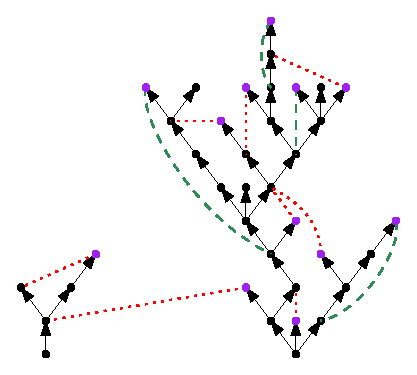
\includegraphics[width=0.7\linewidth]{Content/Pictures/types_of_surplus_edges.eps}
    \caption{This figure illustrates an example of a depth-first exploration of two out-components with the different type of surplus edges highlighted. The ancestral surplus edges (green dashed) point from a vertex $v$ to one of its ancestors. They are always part of a SCC. The other surplus edges are depicted as red dotted lines.}
    \label{subfigure.typesofsurplusedges} 
\end{subfigure}\\
\begin{subfigure}{0.7\textwidth}
  \centering
  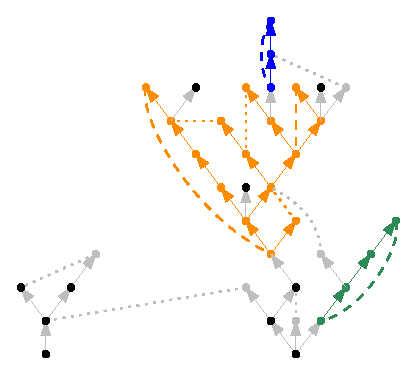
\includegraphics[width=0.7\linewidth]{Content/Pictures/sccs_in_example.eps}
  \caption{The non-trivial SCCs embedded in the components of the out-forest are depicted in orange, blue and green. The trivial SCCs are black. The grey edges are not part of a SCC, and the grey vertices correspond to purple leaves that are not part of a SCC.}
    \label{subfigure.sccinexample}
\end{subfigure}
\caption{We illustrate the different types of surplus edges and how they affect the structure of the SCCs.}
\end{figure}

Corollary \ref{cor.edgesinSCCs} implies that for every purple vertex, we only need to know whether it is a candidate, and if so, where its head is. 
\subsubsection{Sampling the out-forest}\label{subsubsec.samplingoutforest}
This subsubsection discusses how to obtain the out-forest conditional on the order in which the vertices are discovered. We will study the law of the degrees in order of discovery in Subsection \ref{subsec.measurechange}. Informally, the out-forest is obtained in the following way. Let
\begin{equation*}
    \cI_n = \{i \in [n]: D_i^- > 0\}
    \quad \text{and} \quad
    R_n = \abs{\cI_n}
\end{equation*}
such that $R_n$ is the number of vertices with positive in-degree. Suppose the degrees in order of discovery (as given by $\exploredvertices$ in the eDFS algorithm) are given by $(\mathbf{\hat{D}}_{n,1},\dots,\mathbf{\hat{D}}_{n, R_n})$. Up to time step $k$, suppose we have added the vertices corresponding to the first $m\leq k$ elements of  $(\mathbf{\hat{D}}_{n,1},\dots,\mathbf{\hat{D}}_{n, R_n})$ to the forest. We call these vertices \emph{discovered}. Then, at time $k+1$,
\begin{enumerate}
    \item If we have finished a component of the out-forest, let the next out-component have a root with out-degree $\hat{D}_{n,m+1}^+$. 
    \item Otherwise,
    \begin{enumerate}\item With probability proportional to the total in-degree of the undiscovered vertices, i.e. $\sum_{i={m+1}}^n \hat{D}_{n,i}^-$\myworries{check this expression} , let the next vertex in depth-first order be a black vertex with out-degree $\hat{D}_{n,m+1}^+$. 
    \item With probability proportional to the unpaired in-half-edges of the $l$ discovered vertices, let the next vertex in depth-first order be a purple leaf, and reduce the number of unpaired in-edges of the $l$ discovered vertices by $1$.
\end{enumerate}
\end{enumerate}
We make this rigourous in the following lemma.
\begin{lemma}\label{lemma.sampleoutforest}
Suppose the sequence of degrees in order of discovery $(\hat{D}^n_1,\dots,\hat{D}^n_n)$ is given. Suppose, for $1\leq l\leq k$, that up to time $l$, $\hat{P}_n(l)$ surplus edges have been sampled. Then, $$\left(\hat{S}^+_n(l),1\leq l\leq k \right):=\left(\sum_{i=1}^{l-\hat{P}_n(l)}\hat{D}^+_{n,i}-l,1\leq l\leq k\right)$$ is the \L ukasiewicz path of the out-forest up to time $k$. Moreover, for $$\left(\hat{I}^+_n(l),1\leq l\leq k\right):=\left(\min\left\{\hat{S}^+_n(m):1\leq m \leq l\right\},1\leq l \leq k \right),$$
define 
$$\left(\hat{S}^-_n(l),1\leq l \leq k\right):=\left(\sum_{i=1}^{l-\hat{P}_n(l)}\hat{D}^-_{n,i}-l-\hat{I}^+_n(l)+1,1\leq l\leq k\right),$$
so that $\hat{S}^-_n(k)$ is equal to the number of unpaired in-half-edges of discovered vertices at time $k$. Then, the probability that we sample a surplus edge at the $(k+1)^{th}$ time step is given by
$$\frac{\hat{S}^-_n(k+1)}{\sum_{i=1}^n D^-_i-k-\hat{I}^+_n(k)+1}\one_{\left\{\hat{I}^+_n(k)=\hat{I}^+_n(k-1)\right\}}.$$
Therefore, we do not need to know the position of the heads of the surplus edges to sample the out-forest.
\end{lemma}
\begin{proof}
Note that if up to time $k$, $\hat{P}_n(k)$ surplus edges have been sampled, this implies that $k-\hat{P}_n(k)$ vertices have been discovered. Thus, up to time $k$, the out-forest contains $\hat{P}_n(k)$ purple leaves, and black vertices with degrees $(\hat{D}^+_{n,1},\dots,\hat{D}^+_{n,k-\hat{P}_n(k)})$, so by definition of the \L ukasiewicz path, its value is indeed equal to $\hat{S}^-_n(k)$ at time $k$. Moreover, up to time $k$, the total in-degree of the discovered vertices is equal to $\sum_{i=1}^{k-\hat{P}_n(k)}\hat{D}^-_{n,i}$. At every time step, we pair $1$ in-half-edge of a discovered vertex, unless we start a new component. $-\hat{I}^+_n(k)$ corresponds to the number of out-components that are finished up to time $k$, so the total number of unpaired in-half-edges of discovered vertices at time $k$ is equal to $\hat{S}^-_n(k)$. By the same reasoning, the total number of unpaired in-half-edges is equal to $\sum_{i=1}^n D^-_i-k-\hat{I}^+_n(k)+1$. The probability of sampling a surplus edge follows. We note that this probability does not depend on the position of the heads of the surplus edges, which implies that we can sample the out-forest without this information.
\end{proof}
\subsubsection{Sampling the candidates}\label{subsubsec.samplecandidates}
We will now study the law of the candidates conditional on $(\hat{F}_n(k),k\geq 1)$. As before, for each $k$, let $\hat{P}_n(k)$ denote the number of purple vertices amongst the first $k$ vertices in the out-forest, and let $\hat{S}^-(k)$ denote the number of unpaired in-half-edges of discovered vertices at time $k$. We will first identify the tails of the candidates amongst the purple vertices, and then we will sample the position of their heads. \\
If the vertex visited at time $k$ is purple, the head of the corresponding surplus edge is a uniform pick from the $\hat{S}^-(k)$ unpaired in-half-edges of discovered vertices at time $k$. Therefore, the probability that a purple vertex visited at time $k$ corresponds to an ancestral surplus edge is given by the number of unpaired in-edges on its path to the root divided by $\hat{S}^-(k)$. This implies that to understand the law of the position of ancestral surplus edges, we need to understand where the unpaired in-edges are. \\
We will study this by modifying the edge lengths in the tree: for a vertex $v$ with in-degree $m$, the edges connecting it to its children will have length $m-1$ (unless $v$ is the root of an out-component, then the edges connecting to its children will have length $m$). The height of vertex $w$ in this forest with edge lengths corresponds to the number of in-half-edges that can be used to form an ancestral surplus edge with tail $w$. We add lengths to all edges in $(\hat{F}_n(k),k\geq 1)$ and call the resulting forest with edge lengths $(\hat{F}^\ell_n(k),k\geq 1)$. Denote the height process of $(\hat{F}^\ell_n(k),k\geq 1)$ by $(\hat{H}_n^\ell(k),k\geq 1)$. \\
Recall that the first candidate in any component of $(\hat{F}_n(k),k\geq 1)$ is an ancestral surplus edge. The following lemma illustrates the importance of $\hat{H}^\ell$ in finding the first ancestral surplus edges in the out-components.

\begin{lemma}\label{lemma.probancestral}
Consider the exploration of $(\hat{F}_n(k),k\geq 1)$ at time $k$. If no ancestral surplus edge has been sampled in the current component, then the probability that $k$ is the tail of an ancestral surplus edge is given by 
$$a_k=\frac{\hat{H}^\ell(k)}{\hat{S}_n^-(k)}\one_{\{\hat{P}_n(k)-\hat{P}_n(k-1)=1\}}.$$
This event is independent of the position of the heads of the surplus edges that were found before time $k$.
% If $k$ is the tail of an ancestral surplus edge, then the position of the end point $Y$ has the following law. Let $U$ be uniform on $[0,\hat{H}^\ell(k)]$. Then, let $Y_k$ be the height of youngest ancestor $l$ of $k$ such that $H^{\ell}(l)<U$. 
\end{lemma}
\begin{proof}
We claim that if no ancestral surplus edge has been sampled in the current component, none of the ancestors of $k$ are the head of a surplus edge. Indeed, for $x$ an ancestor of $k$, all vertices that are visited since the discovery of $x$ up to time $k$ are descendants of $x$, because $(\hat{F}_n(k),k\geq 1)$ is explored in a depth-first manner. Therefore, any surplus edge with head $x$ sampled up to time $k$ is ancestral. This implies that for $d^-$ the in-degree of $x$, the number of unpaired in-half-edges of $x$ at time $k$ is equal to $d^--1$ (unless $x$ is the root of the out-component, in which case it has $d^-$ unpaired in-half-edges).

Therefore, the number of unpaired in-half-edges corresponding to ancestors of $k$ is equal to $H^\ell(k)$. Moreover, note that, by definition of the purple vertices, $k$ is the tail of a surplus edge if and only if $k$ is purple, i.e. if and only if $\hat{P}_n(k)-\hat{P}_n(k-1)=1$. In that case, the probability that it connects to given unpaired in-half-edge of a visited vertex is equal to $1/\hat{S}_n^-(k)$. The stated probability follows. The independence on the position of the heads of earlier surplus edges is immediate.
\end{proof}

We now illustrate how to find the other candidates in a component of $(\hat{F}_n(k),k\geq 1)$. 
\begin{lemma}\label{lemma.samplecandidates}
Let $T^n_{l_n}$ be a component of $(\hat{F}_n(k),k\geq 1)$ with root $l_n+1$ and component length $\sigma_n$. Suppose the first ancestral surplus edge in $T^n_{l_n}$ corresponds to purple vertex $V^n_1\in [l_n+2,l_n+\sigma_n]$. Let $V^n_1<k\leq l_n+\sigma_n$, and suppose the candidates found up to time $k$ are given by $V^n_1,\dots,V^n_m$. Let $T^{n,\text{mk}}_k$ be the subtree of $T^n_{l_n}$ spanned by $\{l_n+1,V^n_1,\dots,V^n_m,k\}$, and let $\ell(T^{n,\text{mk}}_k)$ be its total length with edge lengths as defined by $(\hat{H}^\ell(m),m\in [l_n+1,l_n+\sigma_n])$. Then, the probability that $k$ is a candidate is given by 
$$\frac{\ell\left(T^{n,\text{mk}}_k\right)-l}{\hat{S}^-(k)}\one_{\{\hat{P}_n(k)=\hat{P}_n(k-1)+1\}}.$$
\end{lemma}
\begin{proof}
Note that if $k$ is purple, it gets paired to a uniform pick from the $\hat{S}^-(k)$ unpaired in-half-edges of discovered vertices. By Definition \ref{def.candidate}, in that case, $k$ is a candidate if and only if its head is in $T^{n,\text{mk}}_k$. Observe that $\ell\left(T^{n,\text{mk}}_k\right)$ is equal to the number of in-half-edges of $T_{k}$ that can be used to form surplus edges. By the definition of a candidate, exactly $m$ of those have been paired: one for each element in $\{V^n_1,\dots,V^n_m\}$. This implies that $\ell\left(T^{n,\text{mk}}_k\right)-m$ of the $\hat{S}^-(k)$ options will cause $k$ to be a candidate.
\end{proof}

Note that the probability that a purple vertex corresponds to a candidate only depends on the out-forest and the number of candidates that have been found in the component so far. The position of the heads of the candidates can be found as follows.
\begin{lemma}\label{lemma.sampleheadcandidates}
Let $T^n_{l_n}$ be a component of $(\hat{F}_n(k),k\geq 1)$ with root $l_n+1$ and component length $\sigma_n$. Suppose its candidates are given by $\{V^n_1,\dots,V^n_{N_n}\}$. Then, for $1\leq i\leq {N_n}$, suppose the heads of the surplus edges corresponding to $V^n_1,\dots,V^n_{i-1}$ are given by $W_1^n,\dots,W^n_{i-1}$ respectively. Then, the in-half-edge that $V^n_{i}$ gets paired to is a uniform pick from the $$\ell\left(T^{n,\text{mk}}_{V^n_i}\right)-(i-1)$$ unpaired in-half-edges of $T^{n,\text{mk}}_{V^n_i}$ that remain. Call the corresponding vertex $W^n_i$.
\end{lemma}
\begin{proof}
Given that $V^n_{i}$ is a candidate, its head will be in $T^{n,\text{mk}}_{V^n_i}$. Then, the distribution follows.
\end{proof}

Lemmas \ref{lemma.sampleoutforest}, \ref{lemma.probancestral}, \ref{lemma.samplecandidates}, and \ref{lemma.sampleheadcandidates} justify the following sampling procedure.
\begin{enumerate}
    \item Sample the out-forest $(\hat{F}_n(k),k\geq 1)$.
    \item Fix $T>0$ and define a counting process $(A_n(k),k\leq \lfloor Tn^{2/3}\rfloor)$, with the probability of an increment at time $k$ given by $$a_k=\frac{\hat{H}_n^\ell(k)}{\hat{S}_n^-(k)}\one_{\{\hat{P}_n(k)-\hat{P}_n(k-1)=1\}}.$$
    \item For $i\geq 1$, set $X_i^n=\min\{k:A_n(k)=i\}$. Define
\begin{align*}L_i^n&=\min\left\{k\geq 1:\hat{S}^{+}_n(k)=\min\{\hat{S}^{+}_n(l):l\leq X_i^n\}\right\}\text{ for }i\geq 1\\
\Sigma_i^n&=\min\left\{k \geq 1: \min\left\{\hat{S}^{+}_n(l):l\leq L_i^n+k\right\} < \min\left\{\hat{S}^{+}_n(l):l\leq X_i^n\right\}\right\}\text{ for }i\geq 1,
\end{align*}
so that for each $i\geq 1$, $\left(\hat{S}^+(k),k\in [L_i^n+1,L_i^n+\Sigma_i^n]\right)$ encodes the out-tree containing $X_i^n$. For each $(l_n,\sigma_n)\in \{(L_i^n,\Sigma_i^n)\}$, let $T^n_{l_n}$ be the tree in $(\hat{F}_n(k),k\geq 1)$ with root $l_n+1$, and do the following.
    \begin{enumerate}
    \item \label{item.procedure3} Set $V_1^n=\min\{m\geq 1:A_n(m)=A_n(g)+1\}$, and find the other candidates $\{V_2^n,\dots ,V_{N_n}^n\}$ according to the procedure described in the statement of Lemma \ref{lemma.samplecandidates}.
    \item \label{item.procedure4} For $V_1^n,\dots, V_{N_n}^n$, sample their heads $W_1^n,\dots ,W_{N_n}^n$ respectively according to the procedure described in the statement of Lemma \ref{lemma.sampleheadcandidates}.
    \item Let $T^{n,\text{mk}}(l_n)$ be the subtree of $T^n_{l_n}$ spanned by $\{l_n+1,V_1^n,\dots ,V_{N_n}^n\}$, say $V_i^n\sim W_i^n$ for each $1\leq i\leq N_n$, and set $M^n_{l_n}:=T^{n,\text{mk}}(l_n)/\sim$, which we note is a directed graph with surplus $N_n$. 
\end{enumerate}
\end{enumerate}
Then, all SCCs of $\vec{G}_n(\nu)$ of which the first candidate is sampled before time $\lfloor Tn^{2/3}\rfloor$ are subgraphs of $\left\{M^n_{L_i^n}, i\geq 1 \right\}$. Call these SCCs, ordered by decreasing size $(C_i^T(n),i\geq 1)$, completed with an infinite repeat of $\mathfrak{L}$. Observe that we may view $M^n_{L_i^n}$ as a finite rooted directed multigraph $M^n_{L_i^n}$ whose edges are endowed with lengths. To be precise, in  $M^n_{L_i^n}$, let the vertex set consist of $L_i^n+1$, $W_i^n$ for $i\leq N_n$, and the branch points $V_i^n\wedge V_j^n$ for $i\neq j\leq N_n$. Then, we obtain $(C_i^T(n),i\geq 1)$ by ordering the SCCs in $\left\{M^n_{L_i^n}, i\geq 1 \right\}$ by decreasing size, and completing the list with an infinite repeat of $\mathfrak{L}$. See Figures \ref{figure.extractSCCs1}, \ref{figure.extractSCCs2} and \ref{figure.extractSCCs3} for an illustration of this procedure.

\begin{figure}
\centering
\begin{subfigure}{.7\textwidth}
 \centering
    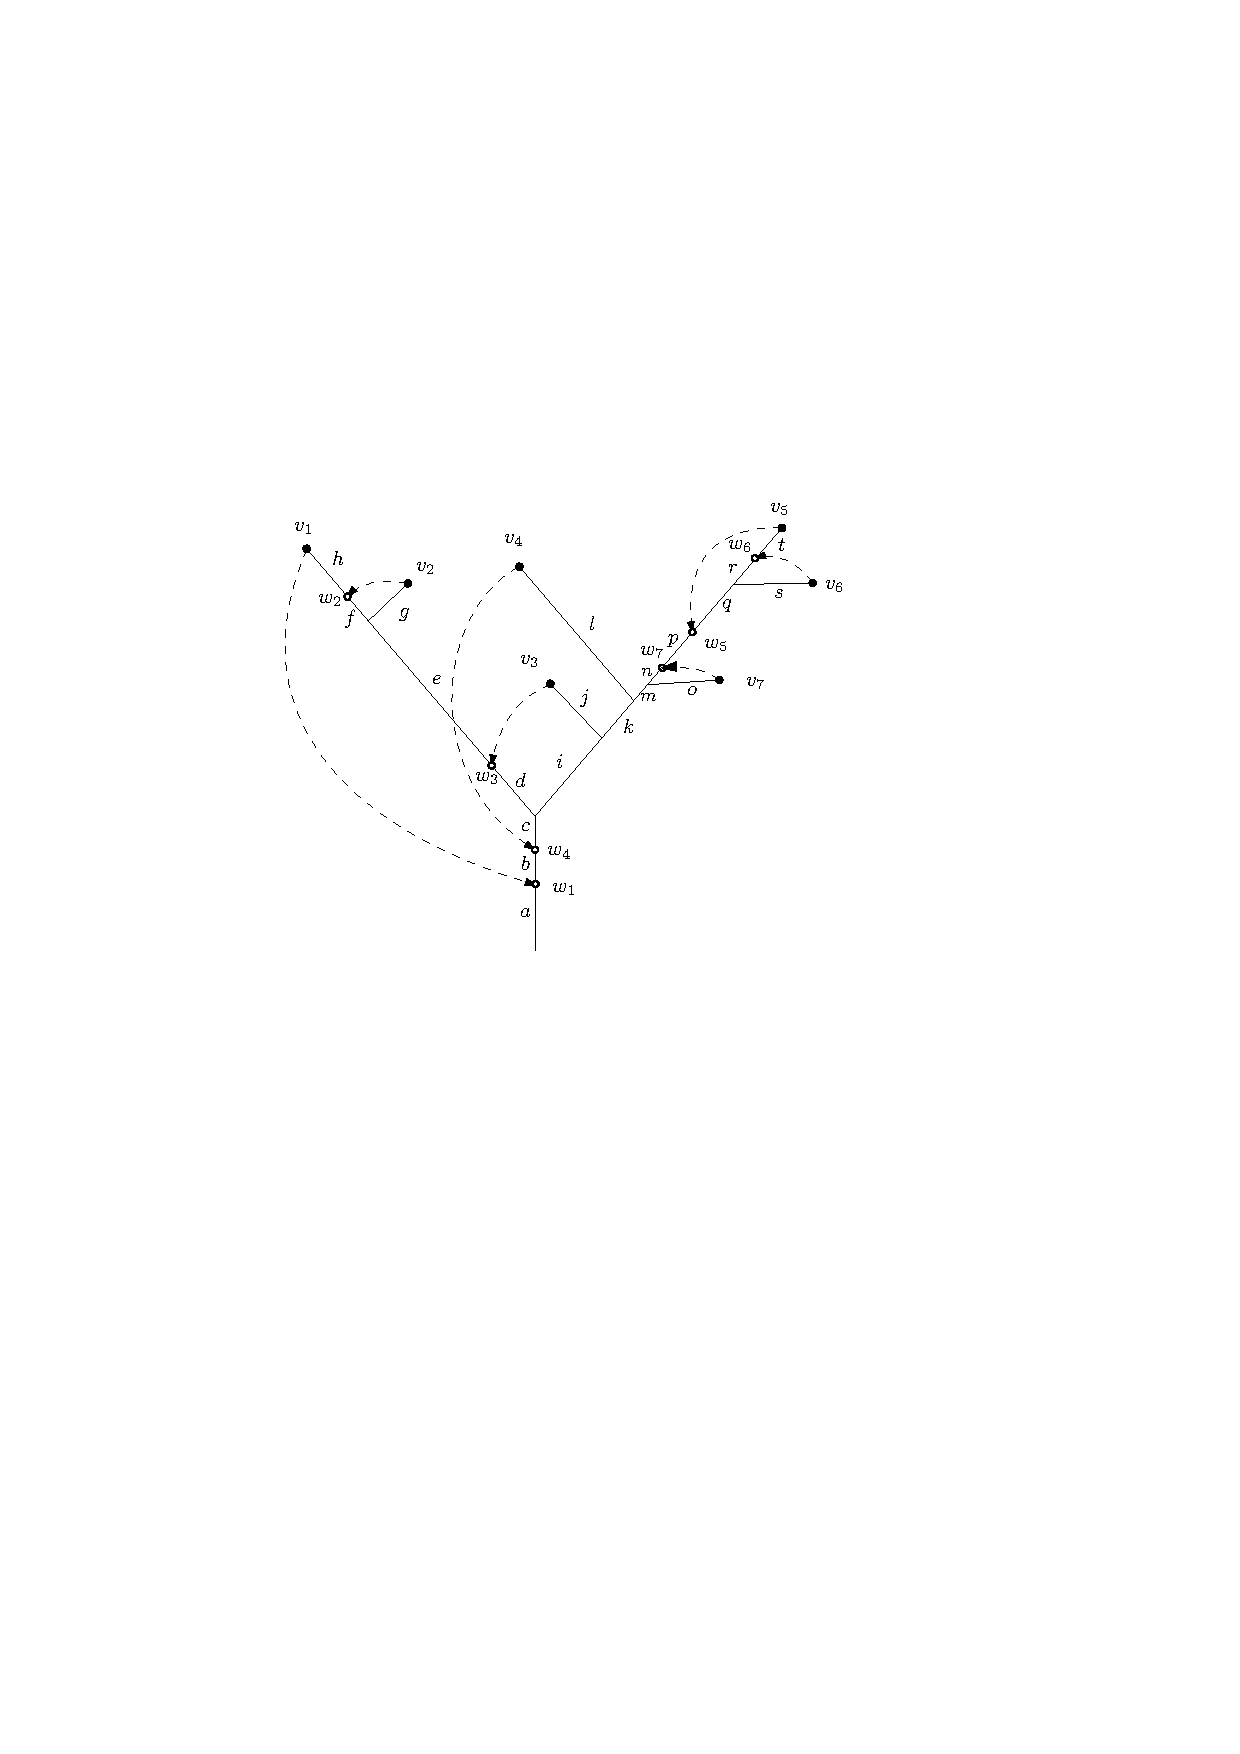
\includegraphics[width=0.8\linewidth]{Content/Pictures/out-componentwithcandidates.pdf}
    \caption{This is a subtree of an out-component spanned by the root of the out-component and the candidate tails $(v_1,\dots,v_7)$. Call the marked tree $T^{\mathrm{mk}}$. The heads of the candidates are denoted by $(w_1,\dots,w_7)$. }
\label{figure.extractSCCs1}
\end{subfigure}\\
\vspace{1.5em}
\begin{subfigure}{.8\textwidth}
  \centering
  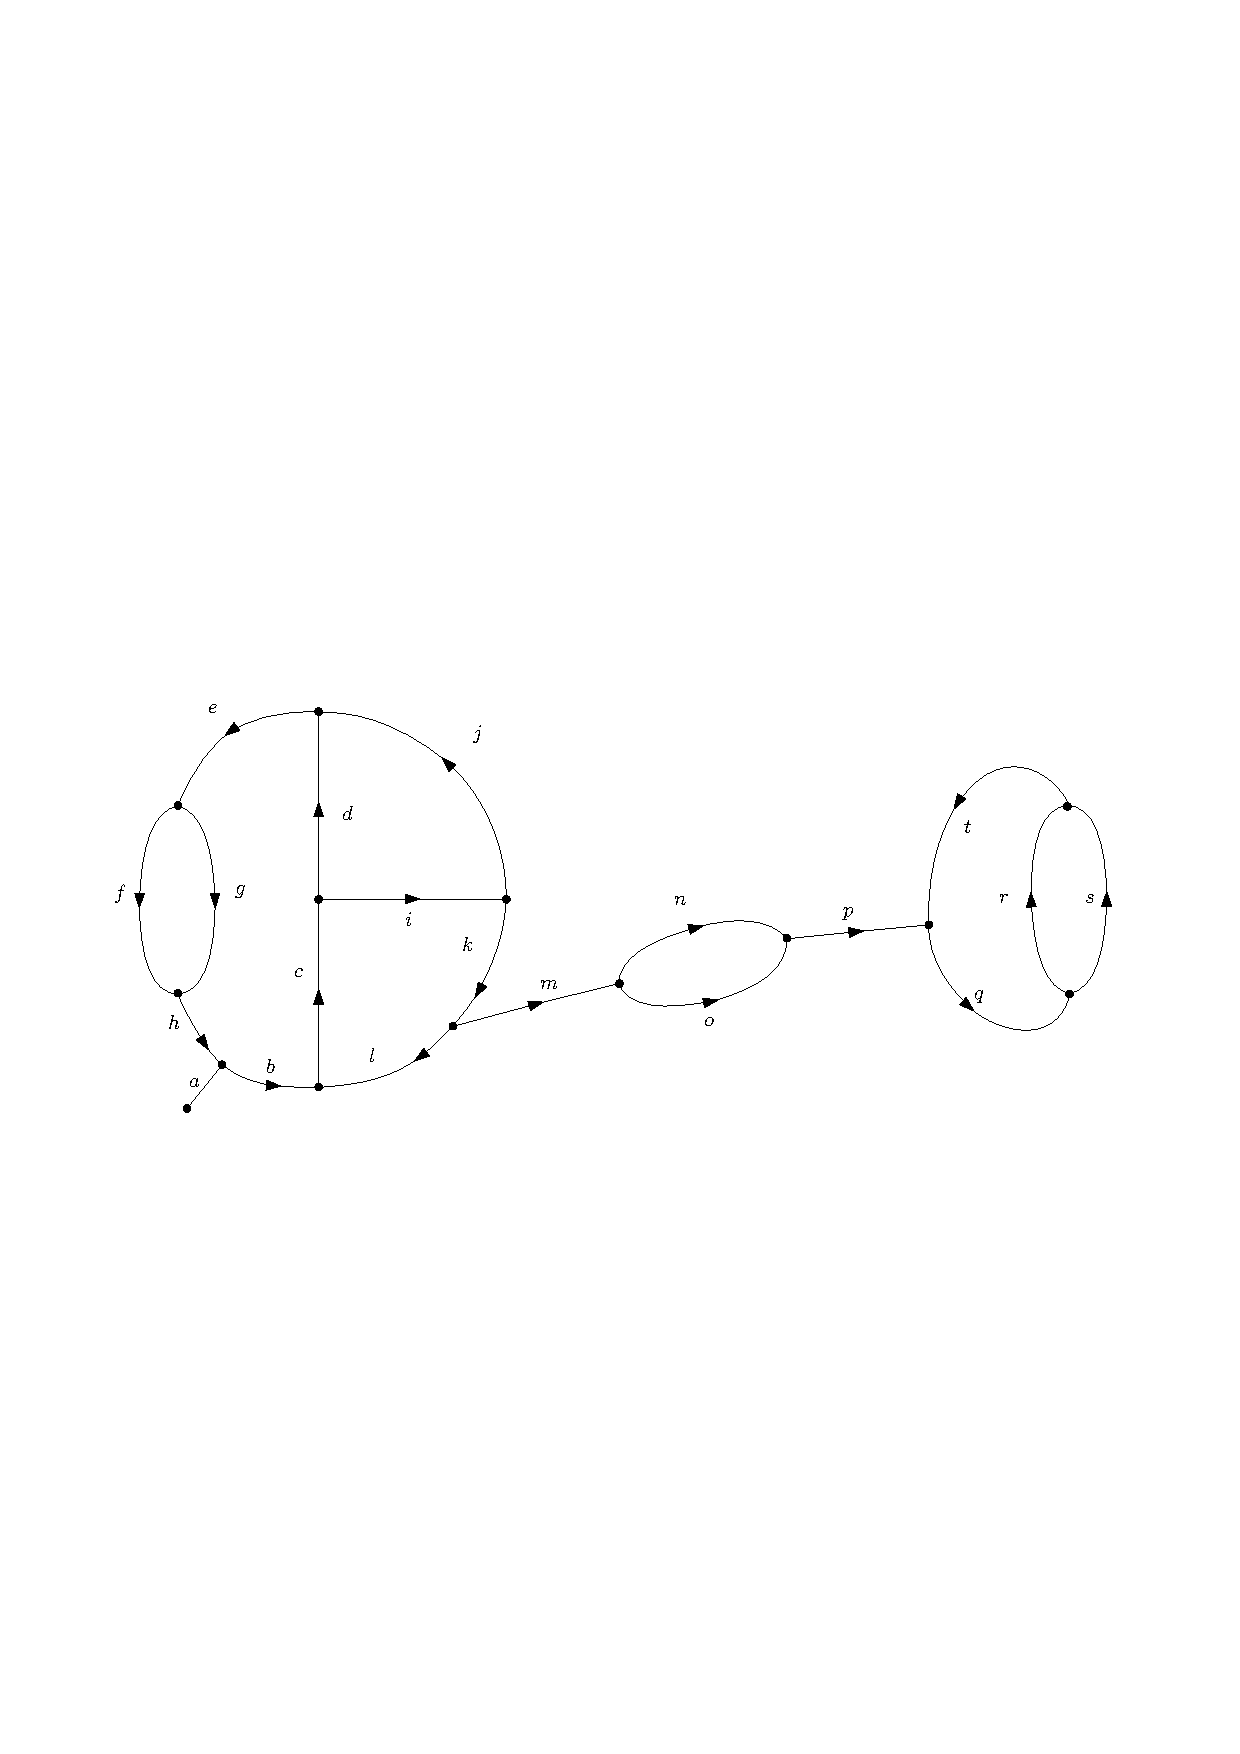
\includegraphics[width=0.9\linewidth]{Content/Pictures/identification.pdf}
  \caption{Identifying $v_i$ with $w_i$ for $i\in [7]$ gives $M$.}
  \label{figure.extractSCCs2}
\end{subfigure}\\
\vspace{1.5em}
\begin{subfigure}{.8\textwidth}
  \centering
  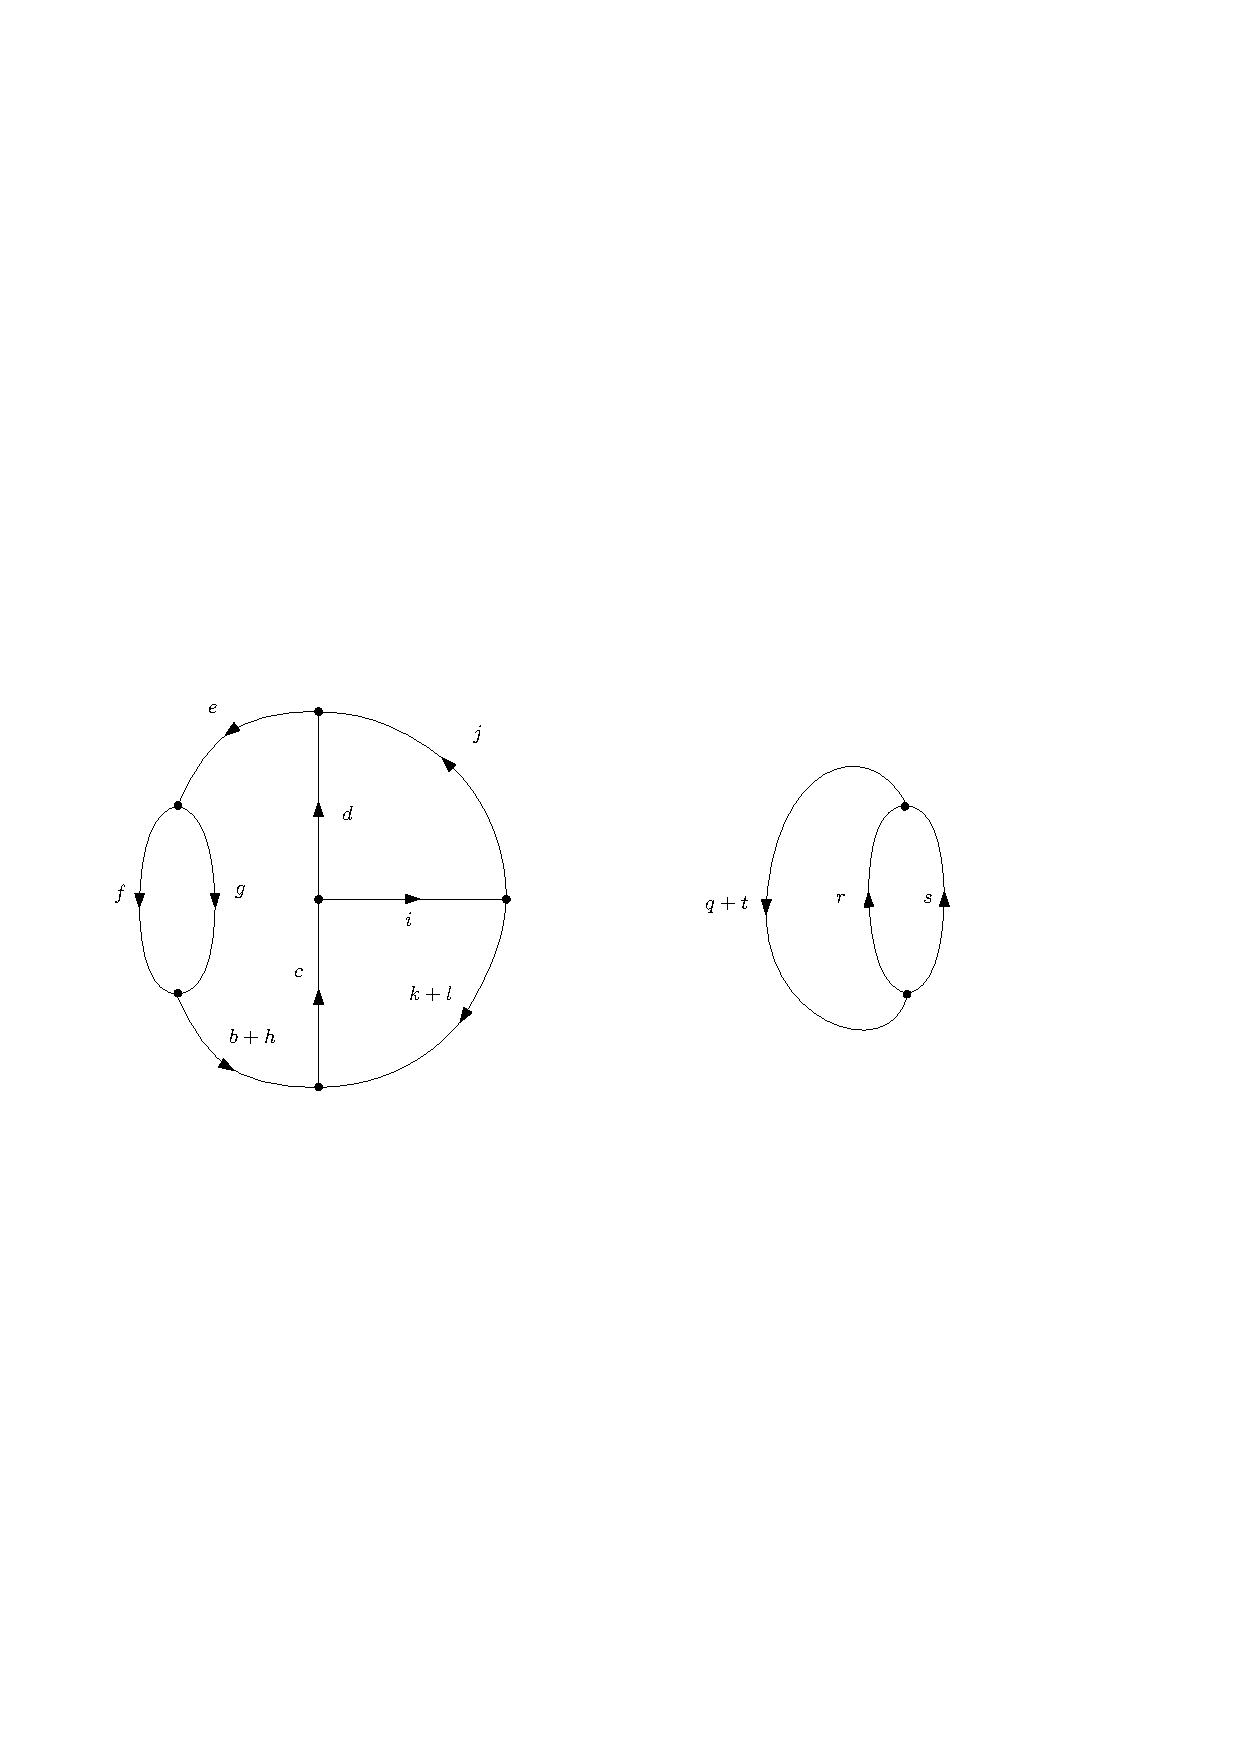
\includegraphics[width=0.9\linewidth]{Content/Pictures/cutting.pdf}
  \caption{We find the SCCs that are contained in $M$.}
  \label{figure.extractSCCs3}
\end{subfigure}

\caption{We illustrate the procedure to find the SCCs in a component of the out-forest after finding the candidates. Source figures: \cite{goldschmidtScalingLimitCritical2019}}
\end{figure}

\subsection{The continuum case}\label{subsec.limitobject}

We will define now define the continuous counterpart of the sampling procedure of the out-forest and the candidates. This is a modification of the procedure defined in Subsubsection 3.2.2 of \cite{goldschmidtScalingLimitCritical2019}. \\

\subsubsection{\texorpdfstring{$\R$}{R}-trees and their encoding}
The continuum analogue of discrete trees are given by $\R$-trees. A survey paper on $\R$-trees can be found in \myworries{insert Le Gall reference}. An $\R$-tree is a compact metric space $(\cT, d)$ such that for every $a, b \in \cT$ the following two properties hold:
\begin{enumerate}
    \item There exists a unique isometry $i_{a, b} : [0, d(a, b)] \to \cT$ such that $i_{a, b}(0) = a$ and $i_{a, b}(d(a, b)) = b$.
    \item If $q: [0, 1] \to \cT$ is any continuous map such that $q(0) = a$ and $q(1) = b$ then the image of $q$ is the same as the image of $i_{a, b}$.
\end{enumerate}
Let $\pathbtw{a, b}$ denote the image of $i_{a, b}$. This is the unique path between $a$ and $b$.

$\R$-trees are often encoded by continuous excursions which can be seen as a continuous analogue of the height function of a tree. Let $f: [0, \sigma] \to [0, \infty)$ be a continuous excursion, meaning $f$ is continuous, $f(0) = f(\sigma) = 0$ and $f(x) > 0$ for all $x \in (0, \sigma)$. Using $f$ we can define a pseudo-metric
\begin{equation*}
    d_f(x, y) = f(x) + f(y) - 2 \min_{s \in [x \wedge y, x \vee y]} f(s).
\end{equation*}
Using this we can define the quotient space
\begin{equation*}
    \cT_f = [0, \sigma] / \{d_f = 0\}.
\end{equation*}
The space $\cT_f$ equipped with the metric $d_f$ is the $\R$-tree encoded by the excursion $f$. Let $p_f: [0, \sigma] \to \cT_f$ be the natural projection function. Then $\cT_f$ inherits a distinguished root vertex $\rho = p(0) = p(\sigma)$.

\subsubsection{The limit object}\label{subsubsec.samplecontinuousobject}
Let $(B_t,t\geq 0)$ be a Brownian motion, and set $$\left(\hat{B}_t,t\geq 0\right)=\left(B_t-\frac{\sigma_{-+}+\nu_-}{2\sigma_+\mu}t^2,t\geq 0\right).$$ 
\begin{remark}
We note that the coefficient of the parabolic drift is negative. Indeed, the sign of the parabolic drift is the same as the sign of $\mu-\E[D^+(D^-)^2]$, and we note that
$$\frac{\E[(D^-)^2D^+]}{\E[D^+]}-\left(\frac{\E[D^+D^-]}{\E[D^+]}\right)^2=\frac{\E[(Z^+)^2]}{\mu}-1$$
is the variance of $D^-$ under the law of $\mathbf{D}$ size-biased by $D^+$, which is positive. Hence $\E[D^+(D^-)^2]/\mu\geq 1$, which shows that $(\hat{B}_t)_{t\geq 0}$ is a Brownian motion with a downwards parabolic drift.
\end{remark}
Define 
$$(\hat{R}_t,t\geq 0)= \left(\hat{B}_t-\inf\left\{\hat{B}_s: s\leq t\right\},t\geq 0\right).$$
Then, it is standard that $\left(\frac{2}{\sigma_+}\hat{R}_t,t\geq 0\right)$ is the height process corresponding to an $\R$-forest with \L ukasiewicz path $\left(\sigma_+\hat{B}_t,t\geq 0\right)$.  This fact also follows from the argument in Section \ref{sec.convoutforest}. Call this forest $(\hat{\cF}(t),t\geq 0)$. \\
Let $(A_t,t\geq 0)$ be a Cox process of intensity $$\frac{2(\sigma_{-+}+\nu_-)}{\sigma_+\mu^2} \hat{R}_t$$ at time $t$. Then, fix $T>0$, so that $A_T<\infty$ almost surely. For $i$ in $\left[A_T\right]$, set $X_i=\min\{t:A_T=i\}$. Define
\begin{align*}
L_i&=\inf\left\{t\geq 0:=\hat{B}_t=\inf\{\hat{B}_s:s\leq X_i\}\right\}\text{ for }i\in \left[A_T\right]\text{ and}\\
\Sigma_i&=\inf\left\{ t\geq 0: \inf\{\hat{B}_s:s\leq L_i+t\} < \inf\{\hat{B}_s:s\leq X_i\}\right\}\text{ for }i\in \left[A_T\right],
\end{align*}
so that for each $i$ in $\left[A_T\right]$, $\left(\frac{2}{\sigma_+}\hat{R}_t,t\in [L_i,L_i+\Sigma_i]\right)$ encodes the $\R$-tree in $(\hat{\cF}(t),t\geq 0)$ that contains $X_i$. For each element of $\{(L_i,\Sigma_i):i\in A_T\}$ we will sample the candidates in the $\R$-tree. Fix $i$, and set $(l,\sigma)=[L_i,\Sigma_i]$. Let $V_1=\inf\{s>0:A(s)=A(l)+1\}$, so that $l\leq V_1\leq l+\sigma$ by definition of $(l,\sigma)$. Let $\cT_l$ be the $R$-tree encoded by $\left(\frac{2}{\sigma_+}\hat{R}_t,t\in [l,l+\sigma]\right)$ and let $p_l:[l,l+\sigma]\to \cT_l$ be the projection onto $\cT_l$ given by the encoding. Set $$||\cT_l||=\sup\left\{\frac{2}{\sigma_+}\hat{R}_t,t\in [l,l+\sigma]\right\},$$
which we note is the height of $\cT_l$. \\
Suppose we have found candidates $\{V_1,\dots,V_m\}$. For $V_m\leq s\leq l+\sigma$, let $T^{\text{mk}}_s$ be the subtree of $\cT_l$ spanned by $p_l\left(\{l,V_1,\dots,V_m,s\}\right)$, and let $|T^{\text{mk}}_s|$ be its total length. Then, let $V_{m+1}$ be the first arrival time of a Poisson process on $[V_m,l+\sigma]$ of intensity $$\frac{\sigma_{-+}+\nu_-}{\mu^2}|T^{\text{mk}}_s|ds.$$ If the process does not contain a point, let $\{V_1,\dots,V_m\}$ be the candidates of $\cT_l$, and set $N=m$. Otherwise, we repeat the inductive step for $\{V_1,\dots,V_{m+1}\}.$ If the induction does not terminate, we set $N=\infty$.\\
We claim that $\P(N=\infty)=0$. Indeed, note that $V_m\leq s\leq V_{m+1}$ implies that  $|T^{\text{mk}}_s|<(m+1)||\cT_l||$. Therefore, 
$$\P\left(\left.N\geq l+1,V_{m+1}-V_m<t \right|N\geq l\right)\leq \P(E_{m+1}<t),$$
for $(E_{k},k\geq 1)$ a sequence of exponential random variables with respective rates $$\frac{\sigma_{-+}+\nu_-}{\mu^2}k||\cT_l||.$$ 
Then,
$$\P\left(N=\infty \right)=\P\left(N=\infty\text{ and }\sup\{c_i:i\in \N\}<l+\sigma\right)\leq \P\left(\sum_{i=2}^\infty E_k\leq l+\sigma-V_1\right).$$
However, $\sum_{i=2}^\infty E_k=\infty$ a.s., because the harmonic series diverges, so, indeed, $\P\left(N<\infty \right)=1$. \\
Finally, for $1\leq i \leq N$, let the head corresponding to $V_i$, which we call $W_i$, be a uniform pick from the length measure on $T^{\text{mk}}_{V_i}$. \\
Let $T^{\text{mk}}_l$ be the subtree of $\cT^{l}$ spanned by $\{l,V_1,\dots,V_N\}$. Then, in $T^{\text{mk}}_{l}$, set $V_i\sim W_i$ for each $1\leq i\leq N$, and set $\cM_{l}:=T^{\text{mk}}_{l}/\sim$. View $\cM_{l}$ as an element of $\vec{\cG}$ in the natural way, and call it $M_l$. To be precise,  let the vertex set of $M_l$ consist of $l$, $W_i$ for $i\leq N$, and the branch points $V_i\wedge V_j$ for $i\neq j\leq N$. The directions are inherited from $\cT^l$, by considering all edges directed away from the root. Remove all edges that do not lie in a SCC of $M_{l}$ and delete any isolated vertices that are thus created. Then, for any vertices of degree $2$, merge the neighbouring edges and sum their lengths. This creates a collection $\cC_l$ of strongly connected MDMs. Doing this for each $(l,\sigma)\in \{[L_i,\Sigma_i]\}$ yields the collection of strongly connected MDMs $\cC$ that has the law of the limit in Theorem \ref{thm.main}.

\subsubsection{Properties of the limit object}
We note that the limit object is encoded by $3$ parameters: the real forest is encoded by a Brownian motion with variance $\sigma_+^2$ and parabolic drift with coefficient $-(\sigma_{-+}+\nu_-)/(2\mu)$, and the identifications are a Cox process with intensity $(\sigma_{-+}+\nu_-)/\mu^2$ on the length measure of the subtree spanned by the previously found candidates and the currently explored point as described in \ref{subsubsec.samplecontinuousobject}. The limit object that is studied in \cite{goldschmidtScalingLimitCritical2019} corresponding to $\lambda=0$ (i.e. at criticality) is equal to our limit object in the case $\sigma_+^2=1$, $-(\sigma_{-+}+\nu_-)/(2\mu)=-1/2$, and $(\sigma_{-+}+\nu_-)/(\mu^2)=1$. Note that these three conditions are satisfied if we let $D^-$ and $D^-$ be independent $\operatorname{Poisson}(1)$ random variables. In \cite{goldschmidtScalingLimitCritical2019}, some properties of the limit object corresponding to these specific parameters are shown. A quick check shows that the proofs do not depend on the values of the parameters, so we deduce that the properties also hold for our limit object. Let $\cM:=\bigcup_{L_i}\cM_{L_i}$.

\begin{corollary}
\begin{enumerate}
    \item The number of complex connected components of $\cM$ has finite expectation.
    \item The number of loops of $\cM$ is a.s. finite.
\end{enumerate}
\end{corollary}
\begin{proof}
The proof is analogous to the proof of Theorem 4.5 in \cite{goldschmidtScalingLimitCritical2019}.
\end{proof}
\begin{corollary}\label{cor.allengthsaredifferent}
The SCCs of $\cM$ all have different lengths almost surely.
\end{corollary}
\begin{proof}
The proof is analogous to the proof of Proposition 4.6 in \cite{goldschmidtScalingLimitCritical2019}.
\end{proof}
Write $\cC$ for the SCCs of $\cM$ and $\mathbf{C}_l$ for those of $\cM_l$, in decreasing order of length, with $\cM_l$ as defined in Subsubsection  \ref{subsubsec.samplecontinuousobject}. Write $\cC_{\text{cplx}}$ for the list of complex components of $\cC$ in decreasing order of length. For sequences $(K_1,\dots, K_j)$ and $(J_1,\dots,J_k)$ of directed multigraphs, write $(J_1,\dots,J_k)\equiv(K_1,\dots, K_j)$ if $j=k$ and $J_i$ is isomorphic to $K_i$ for each $i\leq j$. Extend this notation naturally to the case where one or both of the sequences has edge lengths by ignoring the edge lengths. 
\begin{corollary}
Let $K_1,\dots, K_j$ be a finite sequence consisting of $3$-regular strongly connected directed multigraphs or loops. We have 
$$\P\left[\cC_l\equiv(K_1,\dots, K_j)\right]>0.$$
Assuming that $K_1,\dots, K_j$ are all complex, we also have that 
$$\P\left[ \cC_{\text{cplx}}\equiv(K_1,\dots, K_j)\right]>0.$$
Let $(e_i,1\leq i \leq K)$ be an arbitrary ordering of the edges of $K_1,\dots, K_j$. Then, conditionally on $\cC_l\equiv(K_1,\dots, K_j)$, (resp. $\cC_{\text{cplx}}\equiv(K_1,\dots, K_j)$), $\cC_l$ (resp. $\cC_{\text{cplx}}$) gives lengths $(\ell(e_i),1\leq i \leq K)$ to these edges, and their joint distribution has full support in 
$$\left\{\mathbf{x}=(x_1,\dots, x_K)\in \R_+^K:\forall 1\leq i\leq k-1, \sum_{j:e_j\in E(K_i)}x_j \geq \sum_{j:e_j\in E(K_{i+1})}x_j\right\}.$$
\end{corollary}
\begin{proof}
The proof is analogous to the proof of Theorem 6.1 in \cite{goldschmidtScalingLimitCritical2019}.
\end{proof}


\section{Convergence of the out-forest}\label{sec.convoutforest}
In this section, we will show that the \L ukasiewicz path and height process corresponding to the forest $\hat{F}_n(m_n)$ converge under rescaling, for $m_n=O(n^{2/3})$. 
The main result of this section is as follows. 

\begin{theorem}\label{thm.convoutforest}
As before, let $(\hat{F}_n(k),k\geq 1)$ be the sequence of out-forests given by the exploration, where we set $\hat{F}_n(k+1)=\hat{F}_n(k)$ if all in-half-edges have been paired at time $k$. Let $(\hat{S}^{+}_n(k),\hat{H}_n(k),k\geq 1)$ be the \L ukasiewicz path and height process corresponding to $(\hat{F}_n(k),k\geq 1)$. Let $\hat{S}^-_n(k)$ denote the number of unpaired in-half-edges of vertices that have been discovered at time $k$. Let $\hat{P}_n(k)$ be the number of purple vertices added in the first $k$ time steps. \\
Moreover, let $(B_t)_{t\geq 0}$ be a Brownian motion, and define
$$(\hat{B}_t,t\geq 0):=\left( B_t-\frac{\sigma_{-+}+\nu_-}{2\sigma_+ \mu}t^2, t\geq 0\right).$$ 
Set $$(\hat{R}_t,t\geq 0)= \left(\hat{B}_t-\inf\left\{\hat{B}_s: s\leq t\right\},t\geq 0\right).$$
Then,

\begin{align*}\left(n^{-1/3}\hat{S}^{+}_n\left(\lfloor n^{2/3}t\rfloor \right),n^{-1/3}\hat{H}_{n}\left(\lfloor n^{2/3}t\rfloor \right), t\geq 0\right)
\overset{d}{\to}\left(\sigma_+ \hat{B}_t, \frac{2}{\sigma_+} \hat{R}_t, t\geq 0\right)\end{align*}
in $\D(\R_+,\R)^2$, and 
\begin{align*}\left( n^{-2/3}\hat{S}_n^-\left(\lfloor n^{2/3}t\rfloor \right), n^{-1/3}\hat{P}_n\left(\lfloor n^{2/3}t\rfloor \right), t\geq 0\right)\overset{p}{\to}\left(\nu_-t,  \frac{\nu_-}{2\mu} t^2, t\geq 0\right)\end{align*}
in $\D(\R_+,\R)^2$ as $n\to \infty$. 
\end{theorem}
We prove Theorem \ref{thm.convoutforest} by studying two other forests that are related to $\hat{F}_n(m_n)$ via a change of measure.  \\
The proof is structured as follows.
\begin{enumerate}
    \item \label{item.measurechangeexists} Let $(\mathbf{\hat{D}}_{n,1},\dots,\mathbf{\hat{D}}_{n,R_n})$ denote the degree tuples in order of discovery. Let $\mathbf{Z}_1, \mathbf{Z}_2, \ldots$ be an i.i.d. sequence of $\N\times \N$-valued random variables, $\mathbf{Z}_i:=(Z_i^-,Z_i^+)$ such that 
    $$\P(Z_i^-=k^-, Z_i^+=k^+)=\frac{k^-\P(D^-=k^-,D^+=k^+)}{\mu}.$$
    Then, we show that the law of $(\mathbf{\hat{D}}_{n,1},\dots,\mathbf{\hat{D}}_{n,m})$ conditional on $\sum_{i=1}^n D_i^-=\sum_{i=1}^n D_i^+$ and $m \leq R_n$ is absolutely continuous to $(\mathbf{Z}_1,\dots, \mathbf{Z}_m)$, and we show the convergence of the Radon-Nikodym derivative $\phi_m^n$ for $m=O(n^{2/3})$. This is the content of Subsection \ref{subsec.measurechange}.
    \item Then, \ref{item.measurechangeexists} is the motivation to sample i.i.d. copies of $\mathbf{Z}$, $(\mathbf{Z}_i,i\geq 1)$, and to study a Galton-Watson forest with offspring distributed as $Z_1^+$. Call this forest $(F(k),k\geq 1)$. The convergence of the \L ukasiewicz path of $(F(k),k\geq 1)$ under rescaling follows from Donsker's theorem.
    \item In Subsection \ref{subsec.purpleleavesGWforest}, we modify $(F(k),k\geq 1)$ to include purple leaves. We add extra randomness, similarly to the procedure described in Lemma \ref{lemma.sampleoutforest}, such that at some time steps, a purple leaf is added. We call the resulting forest $(F^p_n(k),k\geq 1)$. We respect the order of the degrees in $(F(k),k\geq 1)$, in the sense that for any $k$, the $k^{th}$ black vertex in $(F^p_n(k),k\geq 1)$ has the same number of children as the $k^{th}$ vertex in $(F(k),k\geq 1)$. $(F^p_n(k),k\geq 1)$ depends on $n$, because the probability of finding a purple vertex depends on $n$. We then show that the \L ukasiewicz path and height process corresponding to $(F^p_n(k),k\geq 1)$ converge under rescaling, jointly with the convergence of the \L ukasiewicz path and height process corresponding to $(F(k),k\geq 1)$ under rescaling up to time $O(n^{2/3})$.
    \item We use the measure change to translate the convergence of the encoding processes of $(F^p_n(k),k\geq 1)$ under rescaling to the convergence of the encoding processes of $(\hat{F}_n(k),k\geq 1)$ under rescaling up to time $O(n^{2/3})$. This yields Theorem \ref{thm.convoutforest}. 
\end{enumerate}

\subsection{The measure change and its convergence}\label{subsec.measurechange}

The following lemma asserts existence of the measure change and gives the scaling limit of the measure change, jointly with the random walks $Y^-$ and $Y^+$. The measure change is under the conditioning $m \leq R_n$ which is an event that occurs with high probability when $m = \Theta(n^{2/3})$.

\begin{restatable}{lemma}{measurechange}
    \label{lem:measure-change}
    For all $m \leq n$ there exists a function $\phi^n_m: (\N \times \N)^m \to \R$ such that 
    \begin{equation*}
        \E\left[ 
            u\left( 
                \hat{\vD}_{n, 1}, \ldots, \hat{\vD}_{n, m}
             \right) 
             \,\middle\vert\,
             m \leq R_n, \Delta_n = 0
         \right]
        =
        \E\left[ 
            u\left( 
                \vZ_1, \ldots, \vZ_m
             \right)
             \phi^n_m(\vZ_1, \ldots, \vZ_m)
         \right].
    \end{equation*}
    for all bounded measurable test functions $u: (\N \times \N) \to \R$. Define
    \begin{align*}
        \Phi(n, m) = \phi^n_m(\vZ_1, \ldots, \vZ_m).
    \end{align*}
    Further let $(W^-, W^+)$ be a pair of standard correlated Brownian motions with correlation $\corr(Z^-_i, Z^+_i)$ and define
    \begin{equation*}
        \Phi(t) = \exp \left( 
            - \frac{\sigma_-}{\mu} \int_0^t s \dif W^-_s - \frac{\sigma_-^2}{6 \mu^2} t^3
         \right).
    \end{equation*}
    Then for all $T > 0$,
    \begin{equation*}
        \left( 
            \Phi(n, \floor{T n^{2/3}}), \left( n^{-1/3} Y^+\left( \floor{n^{2/3} t} \right) \right)_{t \in [0, T]}
        \right)
        \todist
        \left( 
            \Phi(t),
            (\sigma_+ W^+_t)_{t \in [0, T]}
        \right)
    \end{equation*}
    in $\R \times \D([0, T], \R)$ as $n \to \infty$. Moreover $(\Phi(n, \floor{T n^{2/3}}))_{n \geq 1}$ is a uniformly integrable sequence of random variables.
\end{restatable}

\subsection{Convergence of the degrees in order of discovery}
Recall that
$$ \hat{Y}^+(k)=\sum\limits_{i=1}^k (\hat{D}^+_{n,i}-1)$$
encodes the out-degrees in order of discovery, while 
$$ \hat{Y}^-(k)=\sum\limits_{i=1}^k (\hat{D}^-_{n,i}-1)$$
encodes the in-degrees in order of discovery.
 We will study these processes via the measure change that we defined in Subsection \ref{subsec.measurechange}. 
 
%  Recall that 
%  $$ {Y}^+(k)=\sum\limits_{i=1}^k (Z^+_i-1),$$ 
%  and 
%  $$ {Y}^-(k)=\sum\limits_{i=1}^k (Z^-_i-1).$$ 
%  Then, Donsker's theorem and the law of large numbers imply the following straightforward lemma.
% \begin{lemma}
% \label{lem.jointconvergenceinout}
%  We have $$ \left(n^{-2/3}{Y}^-\left(\lfloor n^{2/3}t\rfloor\right), t\geq 0\right)
%  \overset{p}{\to} 
%  \left(\nu_-t, t\geq 0 \right)$$
%  in $\D(\R_+,\R)^2$ as $n\to \infty$.  Moreover,
%  \begin{align*} &\left(n^{-1/3}\left({Y}^-\left(\lfloor n^{2/3}t\rfloor\right)-n^{2/3}\nu_-t\right),n^{-1/3}Y^+\left(\lfloor n^{2/3}t\rfloor\right), t\geq 0\right)\\
%  &\overset{d}{\to} 
%  \left(\mathbf{B}_t, t\geq 0 \right)\end{align*}
%  in $\D(\R_+,\R)^2$, as $n\to \infty$, with $(\mathbf{B}_t,t\geq 0)$ a Gaussian process with covariance matrix
%  $$\begin{pmatrix} \sigma_-^2  & \sigma_{-+} \\ \sigma_{-+}  & \sigma_+^2  \end{pmatrix}t.$$
% \end{lemma} 

\begin{theorem}\label{theorem.convaftermeasurechange} 
 For $T>0$,
$$\left(n^{-2/3}\hat{Y}^-\left(\lfloor n^{2/3} t\rfloor\right), n^{-1/3}\hat{Y}^+\left(\lfloor  n^{2/3} t\rfloor\right), 0\leq t \leq T \right) \overset{d}{\to} \left( \nu_- t, \sigma_+\hat{B}_t, 0 \leq t \leq T \right)$$
in the Skorokhod topology as $n\to \infty$, where $(\hat{B}_t, t\geq 0)$ is distributed as follows.
For $F$ a suitable test function, and for $(B_t)_{t\geq 0}$ a Brownian motion,
\begin{align*} &\E\left[F(\sigma_+ \hat{B}_t,0\leq t \leq T)\right]\\&=\E\left[\exp\left(-\frac{\sigma_{-+}}{\sigma_+ \mu} \int_0^T s dB_s -\frac{\sigma_{-+}^2 T^3}{6\sigma_+^2 \mu^2}\right)F(\sigma_+ B_t,   0\leq t \leq T)\right].\end{align*}

\end{theorem}
\begin{proof}
 We recall from the statement of Lemma \ref{lem:measure-change} that $(W^-,W^+)$ is a pair of correlated standard Brownian motions with correlation $\operatorname{Corr}(Z_i^-,Z_i^+)$. 
Let $(B^1_t,t\geq 0)$ and $(B^2_t,t\geq 0)$ be two independent Brownian motions, so that we may define $$(\sigma_-W^-_t,\sigma_+W^+_t,t\geq 0)=\left(\frac{\sigma_{-+}}{\sigma_+}B_t^1+\left(\sigma_-^2-\frac{\sigma_{-+}^2}{\sigma_+^2}\right)^{1/2} B_t^2, \sigma_+ B_t^1, t\geq 0\right).$$ 
 Then, Lemma \ref{lem:measure-change} implies that for $F$ a suitable test function, 
 \begin{align*}&\E\left[F\left(n^{-1/3}\hat{Y}^+\left(\lfloor n^{2/3}t\rfloor\right), 0\leq t \leq T \right) \right]\\\to& \E\left[\exp\left(-\frac{1}{\mu}\int_0^Tsd\left(\frac{\sigma_{-+}}{\sigma_+}B_s^1+\left(\sigma_-^2-\frac{\sigma_{-+}^2}{\sigma_+^2}\right)^{1/2}B_s^2\right) - \frac{T^3 \sigma_-^2}{6\mu^2}\right) F\left(\sigma_+ B_t^1, 0\leq t \leq T\right)\right]\\
 &=\E\left[\exp\left(-\frac{\sigma_{-+}}{\sigma_+ \mu} \int_0^T s dB^1_s -\frac{\sigma_{-+}^2 T^3}{6\sigma_+^2 \mu^2}\right)F(\sigma_+ B^1_t,   0\leq t \leq T)\right].\end{align*}
 For the details of the argument, we refer the reader to the proof of Theorem 4.1 in \cite{conchon--kerjanStableGraphMetric2020}. Then, the fact that $(Y(k),k\geq 1)$ is a random walk with steps of mean $\nu_-$ implies that
 $$\left(n^{-2/3}Y^-\left(\lfloor n^{2/3}t\rfloor\right),t\geq 0\right)\overset{p}{\to}\left(\nu_- t,t\geq 0\right),$$
 and then, by Lemma \ref{lem:measure-change}, also 
 $$\left(n^{-2/3}\hat{Y}^-\left(\lfloor n^{2/3}t\rfloor\right),t\geq 0\right)\overset{p}{\to}\left(\nu_- t,t\geq 0\right).$$
 \end{proof}
 The following lemma characterises the distribution of $(\hat{B}_t, {0\leq t\leq T})$.
 \begin{lemma}\label{lemma.characterizelimitprocess}
 For $(\hat{B}_t, {0\leq t\leq T})$ as in the statement of Theorem \ref{theorem.convaftermeasurechange}, we have  
 $$(\sigma_+ \hat{B}_t, {0\leq t\leq T})\overset{d}{=}\left(\sigma_+ B_t-\frac{\sigma_{-+}}{2\mu}t^2, {0\leq t\leq T}\right)$$
 for $(B_t)_{t\geq 0}$ a Brownian motion.
 \end{lemma}
 \begin{proof}
 Firstly, we have that for any $t\in [0,T]$ and $\theta>0$,
 \begin{align*} \E\left[\exp(-\theta \sigma_+ \hat{B}_t^+)\right] &= \E \left[ \exp\left(-\frac{\sigma_{-+}}{\sigma_+ \mu}\int_0^t s dB_s-\frac{\sigma_{-+}^2 t^3}{6\sigma_+^2\mu^2}-\theta\sigma_+ B_t  \right)\right]\\
 &=\E\left[\exp \left( -\frac{\sigma_{-+}}{\sigma_+ \mu}\int_0^t \left(s+\frac{\sigma_+^2\theta \mu}{\sigma_{-+}}\right) dB_s -\frac{\sigma_{-+}^2 t^3}{6\sigma_+^2\mu^2}\right)\right] \\
 &= \exp\left(-\frac{\sigma_{-+}^2}{2\sigma_+^2 \mu^2}\int_0^t \left(s+\frac{\sigma_+^2\theta \mu}{\sigma_{-+}}\right)^2 ds -\frac{\sigma_{-+}^2 t^3}{6\sigma_+^2\mu^2}\right)\\
 &=\exp\left(\frac{\sigma_+^2 t}{2}\theta^2+\frac{\sigma_{-+} t^2}{2\mu}\theta \right)\\
 &= \E \left[\exp\left(-\theta\left(\sigma_+ B_t - \frac{\sigma_{-+}}{2\mu} t^2\right)\right)\right]
 \end{align*}
 for $(B_t)_{t\geq 0}$ a Brownian motion.
 Then, more generally, for $m>0$, $0=t_0\leq t_1\leq \cdots \leq t_m=T$, and $\theta_1, \dots, \theta_m \in \R_+$, 
 \begin{align*}
     &\E\left[\exp\left(-\sum_{i=1}^m \theta_i(\sigma_+\hat{B}_{t_i}-\sigma_+\hat{B}_{t_{i-1}})\right)\right]\\
    %  &=\E \left[ \exp\left(-\frac{\sigma}{\mu} \sum_{i=1}^m \int _{t_{i-1}}^{t_i} s dB_s^1-\frac{\sigma_-^2}{2\mu^2}\sum_{i=1}^m \int_{t_{i-1}}^{t_i}s^2ds-\frac{ \sigma_{-+}}{\sigma} \sum_{i=1}^m \theta_i(B_{t_i}^1-B_{t_{i-1}}^1)- 
    %  \left(\sigma_+^2-\frac{\sigma_{-+}^2}{\sigma_-^2}\right)^{1/2}\sum_{i=1}^m \theta_i(B_{t_i}^2-B_{t_{i-1}}^2)\right)\right]\\
     &= \prod_{i=1}^m \E\left[\exp\left(-\frac{\sigma_{-+}}{\sigma_+\mu} \int _{t_{i-1}}^{t_i} s dB_s-\frac{\sigma_{-+}^2 (t_i^3-t_{i-1}^3)}{6\sigma_+^2 \mu^2}-\theta_i \sigma_+  (B_{t_i}-B_{t_{i-1}})\right)\right]\\
     &= \prod_{i=1}^m  \exp\left( -\frac{\sigma_{-+}^2}{2\sigma_+^2 \mu^2}\int_{t_{i-1}}^{t_i}\left(s+\frac{\sigma_+^2\theta_i\mu}{\sigma_{-+}}\right)^2 ds - \frac{\sigma_{-+}^2 (t_i^3-t_{i-1}^3)}{6\sigma_+^2 \mu^2} \right)\\
     &=  \prod_{i=1}^m \exp\left(\frac{ \sigma_+^2 (t_i-t_{i-1}) }{2}\theta_i^2+\frac{\sigma_{-+} (t_i^2-t_{i-1}^2)}{2\mu}\theta_i \right)\\
     &=\E \left[\exp\left(-\sum_{i=1}^m\theta_i\left(\sigma_+ (B_t-B_{t_i}) - \frac{\sigma_{-+}}{2\mu} (t_i^2-t_{i-1}^2)\right)\right)\right],
 \end{align*}
 which proves the result.
 \end{proof}
\subsection{Adding purple vertices to a Galton-Watson forest}\label{subsec.purpleleavesGWforest}
In this subsection we define $(F_n^p(k),k\geq 1)$  and show that its \L ukasiewicz path and height process converge under rescaling. Moreover, we will show that this convergence holds jointly with the convergence under rescaling of the number of purple vertices added up to time $k$ and the number of discovered, but unused in-half-edges up to time $k$. The following lemma motivates the definition of $(F_n^p(k),k\geq 1)$.
\begin{lemma}
Consider an eDFS of a configuration model on $n$ vertices, with the total number of in-half-edges equal to $\mu n$. Suppose the number of unpaired in-half-edges of discovered vertices at step $k$ in the exploration is equal to $S_n^{-}(k)$, suppose $(S_n^{+}(l),1\leq l\leq k)$ encodes the \L ukasiewicz path of the out-forest up to time $k$, and set $$I_n^{+}(k)=\inf\left\{S_n^{+}(l),1\leq l\leq k\right\}.$$
Then, the probability that, in the $(k+1)^{th}$ time step, we sample a surplus edge is given by
$$p_{k+1}:=\frac{S_n^{-}(k)}{\mu n - k -I^{+}(k)+1}\one_{\{I^{+}(k)=I^{+}(k-1)\}}.$$
\end{lemma}
\begin{proof}
This is a slight adaptation of Lemma \ref{lemma.sampleoutforest}, with $(\mathbf{\hat{D}}_{n,1},\dots,\mathbf{\hat{D}}_{n,m})$ replaced by $(\mathbf{Z}_1,\dots, \mathbf{Z}_m)$, and $\sum_{i=1}^n \hat{D}^-_i$ replaced by its mean $\mu n$.
\end{proof}

We will now define $(F_n^p(k),k\geq 1)$ and its \L ukasiewicz path $(S_n^{+}(k), k\geq 1)$ as a function of $(Y^-(k), Y^+(k) ,k\geq 1)$ and extra randomness.
\begin{enumerate} 
    \item Set $P_n(1)=0$, $S_n^{+}(1)=Z_1^+-1$, $S_n^{-}(1)=Z_1^-$. 
    \item Suppose we are given $(P_n(l),S_n^{+}(l),S_n^{-}(l), 1\leq l \leq k)$. Define 
    $I^{+}(k)=\min\{S_n^{+}(l), l\leq k\}$. Then, with probability $p_{k+1}$, independent from everything else, set $P_n(k+1)=P_n(k)+1$. Otherwise, set $P_n(k+1)=P_n(k)$. 
    \item Set $$S_n^{+}(k+1)=Y^+(k+1-P_n(k+1))-P_n(k+1),$$ and $$S_n^{-}(k+1)=Y^-(k+1-P_n(k+1))-P_n(k+1)-I^{+}(k)+1.$$
\end{enumerate}
Let $(F^p_n(k),k\geq 1)$ be the forest with \L ukasiewicz path $(S_n^{+}(k), k\geq 1)$ in which the $k^{th}$ vertex is purple if and only if $P^n(k)-P^n(k-1)=1$. 
\subsubsection{Convergence of the \L ukasiewicz path}
To show the convergence of the \L ukasiewicz path corresponding to $(F^p_n(k),k\geq 1)$, we will first examine the limit of $(P_n(k), k\geq 1)$ under rescaling. We will first prove tightness, after which we will show convergence.


\begin{lemma}\label{lemma.tightnesssurplusedges}
 For every $T>0$, $$\left(n^{-1/3}P_n\left(\lfloor  n^{2/3}T\rfloor \right) \right)_{n\geq 1}$$ 
 is tight.
 \end{lemma}
 \begin{proof}
Set $m=\lfloor  n^{2/3}T\rfloor$ and fix $\epsilon>0$. It is trivial that for any $k\leq m$, $S^{-}(k)\leq \sum_{i=1}^k Z^-_i=Y^-(k)+k$. Moreover, $\mu n - k -I^{+}(l)+1>\mu n-k$.  Therefore, $$p_k\leq \frac{Y^-(k)+k}{\mu n - k},$$
and note that this upper bound is increasing in $k$. Consequently, conditional on $(Y^+(j),Y^-(j),j\geq 1),$ $n^{-1/3}P_n(m)$ is stochastically dominated by a binomial random variable with parameters  $m$ and $$\frac{Y^-(m)+m}{\mu n - m}\wedge 1.$$
Since $(Y^-(k)+k,k\geq 1)$ is a random walk with steps of finite mean, $\left(n^{-2/3}(Y^-(m)+m)\right)_{n\geq 1}$ is tight. Therefore,
$$\left(n^{1/3} \frac{Y^-(m)+m}{\mu n - m}\right)_{n\geq 1}$$ is tight, which proves the statement.
\end{proof}
\begin{lemma}\label{lemma.convergenceQandP}
We have  
$$\left(n^{-1/3}P_n(\lfloor n^{2/3}t\rfloor), t \geq 0\right)\overset{p}{\to} \left(\frac{\nu_-}{2\mu} t^2, t\geq 0\right)$$
in $D(\R_+,\R)$ as $n\to \infty$.

\end{lemma}
\begin{proof}
Fix $T>0$. Recall that
$$p_{k+1}=\frac{S_n^{-}(k)}{\mu n - k -I^{+}(k)+1}\one_{\{I^{+}(k)=I^{+}(k-1)\}}.$$
Define $M^+(k)=\min\{Y^+(l):l\leq k\}$ so that $0\geq I^{+}(k)\geq M^+(k)-P_n(k)$.  Then, by Lemma \ref{lemma.tightnesssurplusedges}, the convergence under rescaling of $Y^+$ shown in Lemma \ref{lem:measure-change}, and the continuous mapping theorem, $\left(n^{-1/3}I^+(\lfloor n^{2/3} t \rfloor)\right)_{n\geq 1}$ is tight for all $t>0$.
We will now argue that the indicator, which ensures that the roots are never purple, does not have an effect on $(P_n(k),k\leq m)$ on the scale that we are interested in. Let $t>0$, and set $m=\lfloor n^{2/3}t\rfloor$. Define
\begin{align*}\begin{split}
E^p(m):&=\sum_{k=0}^{m-1}\frac{S_n^{-}(k)}{\mu n - k -I^{+}(k)+1}\one_{\{I^{+}(k)\neq I^{+}(k-1)\}}\\
&\leq I^{+}(m) \frac{Y^-(m)+m}{\mu n - m},\end{split}\end{align*}
so since $I^{+}(m)$ is of order $n^{1/3}$ and $\frac{Y^{-}(m)+m}{\mu n - m}$ is of order $n^{-1/3}$, $(E^p(m))_{n\geq 1}$ is tight for all $t\geq 0$.  This means that if we allow the roots to be purple, with high probability, we would only sample $O(1)$ purple roots up to time $O(n^{2/3})$. This does not affect $(P_n(k),k\leq m)$ on the scale that we are interested in. \\
 Then, the convergence under rescaling of $Y^-$ and $Y^+$ shown in Lemma \ref{lem:measure-change}, the tightness of $\left(n^{-1/3}I^{+}(\lfloor n^{2/3} t \rfloor)\right)_{n\geq 1}$ and Lemma \ref{lemma.tightnesssurplusedges} imply that
\begin{align}\begin{split}\label{eq.convergenceprob}
  &\left(n^{1/3}\frac{S_n^{-}\left(\lfloor n^{2/3} t \rfloor\right)}{\mu n - \lfloor n^{2/3} t \rfloor -I^{p,+}\left(\lfloor n^{2/3} t \rfloor\right)+1},t\geq 0\right)\\
 &=\left(n^{1/3}\frac{Y^-\left[\lfloor n^{2/3} t \rfloor-P_n\left(\lfloor n^{2/3} t \rfloor\right)\right]-P_n\left(\lfloor n^{2/3} t \rfloor\right)-I^{+}\left(\lfloor n^{2/3} t \rfloor\right)+1}{\mu n - \lfloor n^{2/3} t \rfloor -I^{+}\left(\lfloor n^{2/3} t \rfloor\right)+1},t\geq 0\right)\\
 &\overset{p}{\to} \left(\frac{\nu_-}{\mu}t,t\geq 0\right)\end{split}\end{align}
in $D(\R_+,\R)$ as $n\to \infty$. 
Then, by the continuous mapping theorem and the tightness of $(E^p(m))_{n\geq 1}$,
$$\left(n^{-1/3}\sum_{i=0}^{\lfloor n^{2/3}t \rfloor} p_k , t \geq 0\right)\overset{p}{\to} \left(\frac{\nu_-}{2\mu}t^2,t\geq 0\right)$$
in $D(\R_+,\R)$ as $n\to \infty$. \\
Let $\cG=(\cG_k,k\geq 1)$ denote the filtration such that $\cG_{k}$ contains the information on the shape of the forest until time $k$, including the colours of the vertices. Then, 
$$M_n(k):=\sum_{i=1}^k (\one_{\{P_n(i)-P_n(i-1)=1\}}-p_i)$$ is a martingale in $\cG$. We claim that $(n^{-1/3}M_n(\lfloor n^{2/3} t\rfloor ), t\geq 0)$ converges to $(0,t\geq 0)$ in probability in $D(\R_+,\R)$. Indeed, for any $t\geq 0$,
\begin{align*}\E[n^{-2/3}M_n(\lfloor n^{2/3} t\rfloor )^2]&=n^{-2/3}\sum_{i=1}^{\lfloor n^{2/3} t\rfloor} \E[\E[(\one_{\{P_n(i)-P_n(i-1)=1\}}-p_i)^2|\cG_{i-1}]]\\&=n^{-2/3}\sum_{i=1}^{\lfloor n^{2/3} t\rfloor} \E[p_i-p_i^2]\to 0.\end{align*}
Hence,
$$\left(n^{-1/3}P_n(\lfloor n^{2/3}t\rfloor), t\geq 0\right)=\left(n^{-1/3}\sum_{i=1}^{\lfloor n^{2/3}t\rfloor}  \one_{\{P_n(i)-P_n(i-1)=1\}}  , t\geq 0\right)\overset{d}{\to} \left( \frac{\nu_-}{2\mu}t^2, t\geq 0 \right),$$
 which proves the statement.

\end{proof}

The convergence of $P_n$ under rescaling implies the convergence of $S^{+}$ and $S^{-}$ under rescaling, which is the content of the following corollary. 

\begin{corollary}\label{cor.lukasiewiczpathpurplevertices}
 Let $(B_t,t\geq 0)$ be a Brownian motion. We have 
 \begin{align*}\left(n^{-1/3}Y^{+}\left(\lfloor n^{2/3}t\rfloor\right), n^{-1/3}S^{+}_n\left(\lfloor n^{2/3}t\rfloor\right), t\geq 0\right)\overset{d}{\to}\left(\sigma_+B_t,\sigma_+B_t-\frac{\nu_-}{2\mu}t^2,  t\geq 0\right)\end{align*}
 in $\D(\R_+,\R)^2$  and 
 $$\left(n^{-2/3}S^{-}_n\left(\lfloor n^{2/3}t\rfloor\right),t\geq 0\right)\overset{p}{\to}\left(\nu_- t,t\geq 0\right)$$
 in $\D(\R_+,\R)$ as $n\to\infty$.
\end{corollary}
\begin{proof}
 This follows from the convergence under rescaling of $Y^+$ and $Y^-$ shown in Lemma \ref{lem:measure-change}, \ref{lemma.convergenceQandP} and the expressions 
 $$S_n^{p,+}(k+1)=Y^+\left[k+1-P_n(k+1)\right]-P_n(k+1),$$ and $$S_n^{p,-}(k+1)=Y^-\left[k+1-P_n(k+1)\right]-P_n(k+1)-I^{+}(k)+1.$$
\end{proof}

\subsubsection{Convergence of the height process}\label{subsubsec.convheightprocess}
We will extend Corollary \ref{cor.lukasiewiczpathpurplevertices} to joint convergence under rescaling with the height process corresponding to $(F^p_n(k),k\geq 1)$, which is the content of this subsection. We prove the following proposition. 
\begin{proposition}\label{prop.convheightprocesspurple}
Let $(H^{+}(k),k\geq 1)$ be the height process corresponding to $(F^p(k),k\geq 1)$. Let $(B_t,t\geq 0)$ be a Brownian motion, and define 
$$({B}^+_t,t\geq 0)=\left(B_t-\frac{\nu_-}{2\mu\sigma_+}t^2,t\geq 0\right).$$ 
Set $$(R^+_t,t\geq 0)=\left({B}^+_t-\inf\left\{{B}^+_s: s\leq t\right\},t\geq 0 \right).$$
Then,

\begin{align*}&\left(n^{-1/3}Y^{+}\left(\lfloor n^{2/3}t\rfloor\right), n^{-1/3}S^{+}_n\left(\lfloor n^{2/3}t\rfloor\right),n^{-1/3}H^{+}_n\left(\lfloor n^{2/3}t\rfloor\right), t\geq 0\right) \\
&\qquad \overset{d}{\to}\left(\sigma_+B_t,\sigma_+{B}^+_t, \frac{2}{\sigma_+} R^+_t,  t\geq 0\right)\end{align*}
 in $\D(\R_+,\R)^3$, and 
 $$\left(n^{-2/3}S^{-}_n\left(\lfloor n^{2/3}t\rfloor\right),t\geq 0\right)\overset{p}{\to}\left(\nu_- t,t\geq 0\right)$$
 in $\D(\R_+,\R)$ as $n\to\infty$.
\end{proposition}

The difficulty in proving this proposition is the fact that $(F^p_n(k),k\geq 1)$ is not a Galton-Watson forest, because the probability of sampling a purple vertex is dependent on the past of the process. The theory of convergence of height processes under rescaling is well-developed for Galton-Watson processes (see e.g. \cite{AST_2002__281__R1_0}), but this is not the case for more general processes.  We will adapt a technique that Broutin, Duquesne and Wang develoved in \cite{broutinLimitsMultiplicativeInhomogeneous2020} to show the convergence of the height process of inhomogeneous random graphs under rescaling. The key idea is that  $(F^p_n(k),k\geq 1)$ itself is not a Galton-Watson forest, but we can embed it in a Galton-Watson forest, say $(F^{pr}(k),k\geq 1)$, which will be equal to $(F^p_n(k),k\geq 1)$ with extra red vertices. We then show convergence under rescaling of the height process corresponding to $(F^{pr}(k),k\geq 1)$, and use this to obtain height process convergence for $(F^p_n(k),k\geq 1)$. \\
We start by defining $(F^{pr}(k),k\geq 1)$. Informally, we obtain $(F^{pr}(k),k\geq 1)$ by modifying $(F^p_n(k),k\geq 1)$ in such a way that the sub-tree consisting of the descendants of a purple vertex has the same law as a sub-tree consisting of the descendants of a black vertex. We do this by sampling extra Galton Watson trees with offspring distributed as $Z^+$, of which we colour all vertices red, and identifying their roots with the purple vertices. The resulting forest is a black-purple-red Galton-Watson forest in which the black-purple forest is embedded. This is illustrated in Figure \ref{fig.blackpurpleredforest}. 

\begin{figure}
    \centering
    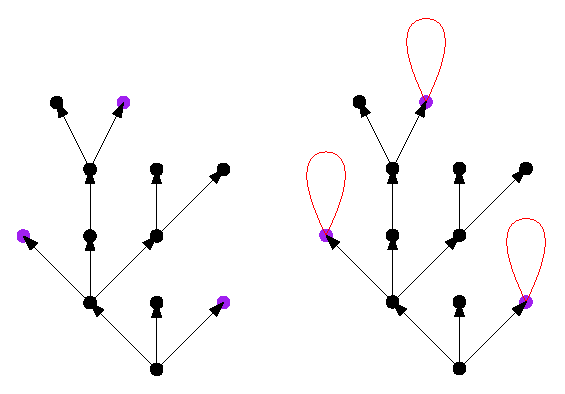
\includegraphics[scale=0.6]{Content/Pictures/black_purple_red_tree.eps}
    \caption{Given a component of $(F^p_n(k),k\geq 1)$ (see left figure), we modify it by sampling independent red Galton-Watson trees with offspring distributed as $Z^+$ and identifying each purple vertex with a root of a red tree. The resulting tree (see right figure) is a Galton-Watson tree, and the resulting forest $(F^{pr}_n(k),k\geq 1)$ is a Galton-Watson forest.}
    \label{fig.blackpurpleredforest}
\end{figure}
The formal procedure is as follows. Suppose we are given $(Y^+(k),S^{+}(k),P_n(k),k\geq 1)$, which encode $(F^p_n(k),k\geq 1)$.
\begin{enumerate}
    \item Let $(Y^{red}(k),k\geq 1)$ be an independent copy of $(Y^+(k),k\geq 1)$. We let $(Y^{red}(k),k\geq 1)$ encode the red pendant subtrees. 
    \item Define $\theta_n(k)=k+\min\{j: Y^{red}(j)=-P_n(k-1)\}-P_n(k-1)$. 
    \item Set $\Lambda_n(k)=\max\{j:\theta_n(j)\leq k\}-P_n(\max\{j:\theta_n(j)\leq k\})$. 
    \item We now define \begin{equation}\label{eq.definitionY^{pr}}(Y^{pr}(k),k\geq 1)=(Y^+(\Lambda_n(k))+Y^{red}(k-\Lambda_n(k)),k\geq 1)\end{equation}
    and we let $(F^{pr}(k),k\geq 1)$ be the Galton-Watson process encoded by $(Y^{pr}(k),k\geq 1)$, in which $P_n(\max\{j:\theta_n(j)\leq k\})$ of the first $k$ vertices are blue, $\Lambda_n(k)$ of the first $k$ vertices are black, and the rest is red. We let $(H^{pr}(k),k\geq 1)$ be the height process corresponding to $(F^{pr}(k),k\geq 1)$.
\end{enumerate}
We claim that the forest consisting of the black and blue vertices in $F^{pr}(\theta_n(k))$ is, by construction, equal to $F^{p}(k)$. Moreover, $(F^{pr}(k),k\geq 1)$ is a Galton-Watson forest. We make the following observations.
\begin{enumerate}
    \item We claim that $$\theta_n(k)=\min\{l: F^p(k)\text{ is a subforest of }F^{pr}(l)\}.$$ Indeed, note that $\min\{j: Y^{red}(j)=-P_n(k-1)\}$ is equal to the number of vertices in the first $P_n(k-1)$ trees in the forest encoded by $Y^{red}$, so $$\min\{j: Y^{red}(j)=-P_n(k-1)\}-P_n(k-1)$$ is equal to the number of red vertices we add to $F^p(k)$. Then, $\theta_n(k)$ is the index in $(F^{pr}(k),k\geq 1)$ of the $k^{th}$ black or purple vertex. 
    \item Note that $\Lambda_n(k)$ is the number of blue vertices amongst the first $k$ vertices. This follows from the fact that $\max\{j:\theta_n(j)\leq k\}$ is the number of blue or purple vertices amongst the first $k$ vertices. 
    \item By the argument above, $(\Lambda_n(k),k\geq 1)$ only takes steps of size $0$ or $1$. Both $(Y^+(k),k\geq 1)$ and $(Y^{red}(k),k\geq 1)$ are random walks with steps distributed as $Z^+-1$, so, by construction, $(Y^{pr}(k),k\geq 1)$ is a random walk with steps distributed as $Z^+-1$, so $(F^{pr}(k),k\geq 1)$ is a Galton-Watson forest with offspring distributed as $Z^+$.
    \item By construction, $(H^{pr}(\theta_n(k)),k\geq 1)$ is the height process corresponding to $(F^p_n(k),k\geq 1)$. Moreover,
   \begin{equation}\label{eq.constructionSp}(S^{+}(k),k\geq 1)=(Y^{pr}(\theta_n(k))-E(\theta_n(k)),k\geq 1),\end{equation}
    where 
    $E(k)$ counts the red children of the $k^{th}$ vertex in $(F^{pr}(k),k\geq 1)$.
\end{enumerate}
Considering the construction above and Corollary \ref{cor.lukasiewiczpathpurplevertices}, in order to prove Proposition \ref{prop.convheightprocesspurple}, it is sufficient to prove the following proposition.
\begin{proposition}\label{prop.heightprocessblackpurplered}
There exists a process $(D_t,t\geq 0)$ such that 
\begin{align*}
    &\left(n^{-1/3}\left[Y^{pr}\left(\theta_n\left(\lfloor n^{2/3}t\rfloor \right)\right)-E\left(\lfloor n^{2/3}t\rfloor \right)\right], n^{-1/3}H^{pr}\left(\theta_n\left(\lfloor n^{2/3}t\rfloor \right)\right),t\geq 0\right)\\
    &\overset{d}{\to}\left(\sigma_+D_t,\frac{2}{\sigma_+}\left(D_t-\inf\left\{D_s,s\leq t\right\}\right),t\geq 0\right)
\end{align*}
in $\D(\R_+,\R)^2$ as $n\to \infty$ and $\left(\frac{2}{\sigma_+}\left(D_t-\inf\left\{D_s,s\leq t\right\}\right),t\geq 0\right)$ is the height process corresponding to $(\sigma_+D_t,t\geq 0)$.
\end{proposition} 
We postpone the proof to Appendix \ref{appendix.heightprocessblackpurplered}. 

\subsection{Applying the measure change to prove Theorem \ref{thm.convoutforest}}\label{subsubsec.convaftermeasurechange}

We will combine the convergence of the measure change under rescaling, which is the content of Lemma \ref{lem:measure-change}, and the convergence of the encoding processes of $(F^p(k),k\geq 1)$, which is the content of Proposition \ref{prop.convheightprocesspurple}, to prove Theorem \ref{thm.convoutforest}.

\begin{proof}[Proof of Theorem \ref{thm.convoutforest}]
Recall that $\hat{P}_n(k)$ denotes the number of purple vertices in $\hat{F}_n(k)$. Set $\hat{I}_n(k)=\min\{\hat{S}^{+}_n(l):l\leq k\}$. Then, as shown in Lemma \ref{lemma.sampleoutforest}, the probability that the $(k+1)^{th}$ vertex in $(\hat{F}_n(k),k\geq 1)$ is purple is given by
$$q_{k+1}:=\frac{\hat{S}^-(k)}{\sum_{i=0}^n D^-_i-k-\hat{I}_n(k)}\one_{\left\{\hat{I}_n(k-1)= \hat{I}_n(k)\right\}}.$$
In order to use the results on $(F^p(k),k\geq 1)$, we would like to replace the term $\sum_{i=0}^n D^-_i$ in the denominator by $\mu n$. Therefore, define a new forest $(\hat{F}'_n(k), k\geq 1)$ in which the probability that the $(k+1)^{th}$ vertex is a purple leaf is
$${q}'_{k+1}:=\frac{\hat{S}^-(k)}{\mu n-k-\hat{I}'_n(k)}\one_{\left\{\hat{I}'_n(k-1)=\hat{I}'_n(k)\right\}},$$
where $\hat{P}'_n(k)$ is the number of purple vertices in $\hat{F}'_n(k)$, and $\hat{I}'_n(k)$ is the number of components in $\hat{F}'_n(k)$. 
We claim that there exists a coupling such that
$$\sum_{i=1}^{\lfloor n^{2/3}T\rfloor }|q_i-q'_i|\overset{p}{\to}0$$
as $n\to \infty$. 
Indeed, by the convergence in Theorem \ref{theorem.convaftermeasurechange}, 
$$\left(n^{-2/3}\sum_{i=1}^{\lfloor n^{2/3}T\rfloor} \hat{D}^n_i\right)_{n>0}$$ is tight. Moreover, with a slight adaptation to the proof of Lemma \ref{lemma.tightnesssurplusedges}, we can show that $\left(n^{-1/3}\hat{P}'_n\left(\lfloor n^{2/3}T\rfloor \right)\right)_{n>0}$ is tight. This, combined with the convergence under rescaling of $(\hat{Y}^+_n(k),k\geq 1)$, implies that also $\left(n^{-1/3}\hat{I}'_n\left(\lfloor n^{2/3}T\rfloor \right)\right)_{n>0}$ is tight.  Since $D^-_1,\dots,D^-_n$ are i.i.d. random variables with mean $\mu$ and finite variance,
$\left(n^{-1/2}\left(\sum_{i=0}^{n-1}D^-_i-\mu n\right)\right)_{n>0}$ is tight. By using the trivial identity $a/b-c/d=(b(a-c)-c(d-b))/bd$, this implies that
$\left(n^{2/3}\max_{k\leq \lfloor n^{2/3}T\rfloor }|q_k-q'_k|\right)_{n>0}$ is tight, which implies that there exists a coupling such that $\left(\max_{k\leq \lfloor n^{2/3}T\rfloor } |\hat{P}_n(k)-\hat{P}'_n(k)|\right)_{n>1}$ and $\left(\max_{k\leq \lfloor n^{2/3}T\rfloor } |\hat{I}_n(k)-\hat{I}'_n(k)|\right)_{n>1}$ are tight, which implies that, again by $a/b-c/d=(b(a-c)-c(d-b))/bd$, 
$\left(n^{5/6}\max_{k\leq \lfloor n^{2/3}T\rfloor }|q_k-q'_k|\right)_{n>0}$ is tight, which implies that 
$$\sum_{i=0}^{\lfloor n^{2/3}T\rfloor }|q_i-q'_i|\overset{p}{\to}0$$
as $n\to \infty$. 
Therefore, under the right coupling, 
$$\P\left(\max_{k\leq \lfloor n^{2/3} T \rfloor}|\hat{P}_n(k)-\hat{P}'(k)|>0\right)\to 0.$$
In other words, we can couple $(\hat{F}_n(k),k\geq 1)$ and $(\hat{F}'_n(k),k\geq 1)$ in such a way that we do not see the difference on the scale that we are interested in. Therefore, we can show convergence under rescaling of the encoding processes of $(\hat{F}'_n(k),k\geq 1)$ instead. To avoid further complicating notation, we will from now on refer to its encoding processes as $$(\hat{S}^{+}_n(k),\hat{H}_n, \hat{S}^-_n(k), \hat{P}_n(k),k\leq \lfloor n^{2/3}T\rfloor).$$ Then, these processes are constructed out of sample paths of $(\hat{Y}^+(k),\hat{Y}^-(k), k\leq \lfloor n^{2/3}T\rfloor )$ and independent randomness in the exact same way as the sample paths of $$({S}_n^{+}(k),{H}_n^+(k),{S}_n^-(k),P_n(k), k \leq \lfloor n^{2/3}T\rfloor )$$ are constructed out of sample paths of $(Y^+(k),Y^-(k), k\leq \lfloor n^{2/3}T\rfloor )$ and independent randomness. 
We will use the following notation:\begin{align*}
    \hat{S}^{+}_{(n)}&:=\left(n^{-1/3}\hat{S}^{+}_n\left(\lfloor n^{2/3} t \right),0\leq t \leq T\right)\\
    \hat{H}_{(n)}&:=\left(n^{-1/3}\hat{H}_n\left(\lfloor n^{2/3} t \right),0\leq t \leq T\right)\\
    \hat{Y}^+_{(n)}&:=\left(n^{-1/3}\hat{Y}^+\left(\lfloor n^{2/3} t \right),0\leq t \leq T\right)\\
     {S}^{+}_{(n)}&:=\left(n^{-1/3}{S}^{+}_n\left(\lfloor n^{2/3} t \right),0\leq t \leq T\right)\\
    {H}^+_{(n)}&:=\left(n^{-1/3}{H}^+_n\left(\lfloor n^{2/3} t \right),0\leq t \leq T\right)\\
    {Y}^+_{(n)}&:=\left(n^{-1/3}{Y}^+\left(\lfloor n^{2/3} t \right),0\leq t \leq T\right).
\end{align*}
Let $f:D([0,T],\R)^3\to \R$ be a bounded, continuous test-function. Then,
\begin{align*}\E\left[f\left(\hat{Y}^+_{(n)}, \hat{S}^+_{(n)},  \hat{H}_{(n)}\right) \right]&= \E\left[ \E\left[\left. f\left(\hat{Y}^+_{(n)},\hat{S}^+_{(n)},  \hat{H}_{(n)}\right)\right|\hat{Y}^+_{(n)}\right]\right]\\&=\E\left[ \Phi(n,\lfloor n^{2/3} T\rfloor)\E\left[\left.f\left(Y^+_{(n)}, S^+_{(n)},  H^+_{(n)}\right)\right| {Y}^+_{(n)}\right]\right]\\&=\E\left[ \Phi(n,\lfloor n^{2/3} T\rfloor)f\left(Y^+_{(n)},S^+_{(n)},  H^+_{(n)}\right)\right],\end{align*}
where we use that $\E\left[\left. f\left(\hat{Y}^+_{(n)},\hat{S}^+_{(n)},  \hat{H}_{(n)}\right)\right|\hat{Y}^+_{(n)}\right]$ is a bounded, adapted function of $\hat{Y}^+_{(n)}$, and that $\Phi(n,\lfloor n^{2/3} t\rfloor)$ is the measure change from ${Y}^+_{(n)}$ to $\hat{Y}^+_{(n)}$. Then, using Lemma \ref{lem:measure-change} and Proposition \ref{prop.convheightprocesspurple}, following the proof of Theorem 4.1 in \cite{conchon--kerjanStableGraphMetric2020} gives us that 
\begin{align*}
    &\E\left[f\left(\hat{Y}^+_{(n)},\hat{S}^+_{(n)},  \hat{H}_{(n)}\right) \right]\\
    &\to \E\left[\Phi(T)f\left(\sigma_+ B_t,\sigma_+ B^+_t,\frac{2}{\sigma_+}R^+_t,0\leq t \leq T\right)\right].
\end{align*}
Since $$(B^+_t,t\geq 0)=\left(B_t-\frac{\nu_-}{2\sigma_+ \mu}t^2,t\geq 0\right),$$
Lemma \ref{lemma.characterizelimitprocess} implies the convergence under rescaling of $(\hat{S}^+_n(k),\hat{H}_n(k),k\geq 0)$. By Proposition \ref{prop.convheightprocesspurple} , $S^{-}_n$ converges in distribution to a deterministic process under scaling, which will not be affected by the measure change. This completes the proof. 
\end{proof}

\subsection{Convergence of the out-forest holds conditionally on the multigraph being simple}
We will now show that the parts of the multigraph we observe up until the timescale in which we are interested are with high probability simple. We will then use an argument by Joseph \cite{josephComponentSizesCritical2014} to show that this implies that Theorem \ref{thm.convoutforest} holds conditional on the resulting multigraph being simple. We let $B_n(k)$ be the number of self-loops and edges created parallel to an existing edge in the same direction as that edge, up until discovery of the $k^{th}$ vertex of $(\hat{F}_n(k),k\geq 1)$. We call these anomalous edges. 
\begin{proposition}\label{prop.anomalousedges}
Suppose $\beta<1$. Then we have
$$\P\left(B_n(\lfloor n^\beta \rfloor)>0\right)\to 0$$
as $n\to \infty$.
\end{proposition}
\begin{remark}
We adapt the proof of Lemma 7.1 of \cite{josephComponentSizesCritical2014} and of Proposition 5.3 of \cite{conchon--kerjanStableGraphMetric2020} to the directed setting. A significant complication is caused by the conditioning on $$\left\{\sum_{i=1}^n D^-_i=\sum_{i=1}^n D^+_i.\right\}.$$ We remark that in both papers, the proof of the aforementioned result is not fully correct, because the authors use a wrong expression for the probability of sampling an anomalous edge. However, the argument below can be adapted to the setting of \cite{josephComponentSizesCritical2014} and \cite{conchon--kerjanStableGraphMetric2020} to yield a correct proof.
\end{remark}
\begin{proof}
Note that we can only show the convergence of the Radon-Nikodym derivative up to time $O(n^{2/3})$, so it is not straightforward to use the measure change to proof results on a time scale $O(n^\beta)$. Therefore, for the proof of this lemma, we will use a different method, that was introduced by Joseph in \cite{josephComponentSizesCritical2014} referred to as \emph{Poissonization}. Let $R_n$ be as before, and conditional on $R_n$, let $D^{0,+}_1,\dots,D^{0,+}_{n-R_n}$ i.i.d.\ random varialbes with the law of $D^+$ conditional on $D^-=0$, and set $S_{n-R_n}=\sum_{i=1}^{n-R_n}$. There is an $L$ such that with high probability, both $R_n$ and $S_{n-R_n}$ are within an interval of width $Ln^{1/2}$ around their mean. We condition on this event. Suppose $R_n=r$ and $S_{n-R_n}=s$, such that the conditioning implies that, in particular, $r=O(n)$. We note that, conditional on $R_n=r$, $(\mathbf{\hat{D}}_{n,1},\dots,\mathbf{\hat{D}}_{r,n})$ (before conditioning on $\sum_{i=1}^nD^-_i=\sum_{i=1}^nD^+_i$) are distributed as the jumps ordered by jump time in a Poisson process $\Pi^0$ with intensity measure $\pi^0$ on $\R_+\times \N^2$ such that $$\pi^0(dt,k_1,k_2)=r\P(D^-=k_1,D^+=k_2|D^->0)k_1\exp(-k_1 t)dt$$
conditional on $\Pi^0(\R,\N,\N)=r$.
The intensity of this process is not constant in $t$, so we perform a time change. Define
$$\cL_{\mathbf{D}}(x,y)=\E\left[\left.\exp(-xD^--yD^+)\right|D^->0 \right],$$
and set 
$$\psi(t)=\left(1-\cL(\cdot,0)\right)^{-1},$$
so that for 
$$\pi_r(dt,k_1,k_2):=\P(D^-=k_1,D^+=k_2)k_1\exp\left(-k_1 \psi(t/r)\right)\psi'(t/r)dt$$
on $(0,r)\times \N^2$, we have that for $t\in (0,r)$, there exists a probability measure $P_t$ on $\N^2$ such that
$$\pi_r(dt,k_1,k_2)=P_t(D^+=k_1,D^+=k_2)dt.$$
This is a trivial adaptation of Lemma 4.1 of \cite{josephComponentSizesCritical2014}. Let ${\Pi}_r$ be a decorated point process with intensity $\pi_r$.  Now, let $\hat{\Pi}_r$ be a random measure, which is a decorated point process with intensity $\pi_r$, conditioned on 
\begin{enumerate}
    \item $N_r:= \hat{\Pi}_r((0,r),\N,\N)=r$, and 
    \item $\Delta_r:=\int_{(0,r)\times \N^2}(k_1-k_2) \hat{\Pi}_r(dt,k_1,k_2)=s$.
\end{enumerate}
Then, the points of $\hat{\Pi}_r$ ordered by time are distributed as $(\mathbf{\hat{D}}_{n,1},\dots,\mathbf{\hat{D}}_{n,r})$ conditional on $\sum_{i=1}^nD^-_i=\sum_{i=1}^nD^+_i$, $R_n=r$ and $S_{n-R_n}=s$. Let $\hat{\pi}^r_t$ be the marginal density of $\hat{\Pi}^r$ at time $t$, so that there is a probability measure $\hat{P}^r_t$ on $\N^2$  and a measure $\lambda^r_t$ on $\R_+$ such that $$\hat{\pi}^r_t(dt,k_1,k_2)=\lambda^r_t(dt)\times \hat{P}^r_t(D^-=k_1, D^+=k_2).$$
Note that due to the conditioning, $\lambda^r_t(dt)$ can be unequal to $dt$. However, we claim that, also after conditioning, with high probability, we will have seen between $n^\beta$ and $3n^\beta$ jumps at time $2n^{\beta}$. Indeed,
\begin{align}\begin{split}\label{eq.numberofjumpsinrandommeasure}\P\left(\left.\Pi_r\left((0,2n^{\beta}),\N,\N\right)\not\in (n^\beta,3n^\beta)\right|\Delta_n=0, N_n=n\right)&\leq \frac{\P\left(\sum_{i=1}^{n^\beta}E_i>2n^{\beta}\text{ or }\sum_{i=1}^{3n^\beta}E_i<2n^{\beta}\right)}{\P(\Delta_r=s, N_r=r)}\\
&=O(n^{1/2}\exp(-n^\beta))\end{split}\end{align}
for $(E_1,E_1,\dots)$ i.i.d. exponential random variables with rate $1$, where the order follows from Cramér's Theorem and the local limit theorem (recall that we conditioned $r$ and $s$ to be at distance $O(n^{1/2})$ from the mean of $R_n$ and $S_{n-R_n}$ respectively). \\
We will use this set-up to show that with high probability, we do not sample anomalous edges in the first $n^\beta$ time steps of the eDFS. We distinguish between the following types of anomalous edges.\\
Self-loops occur when the out-half-edge of a vertex is paired to an in-half-edge of the same vertex.  Let $B^1_n(k)$ be the number of self-loops that are found up to time $k$. For $v$ explored up to time $\lfloor n^\beta\rfloor$, a vertex with in-degree $d^-_v$ and out-degree $d^+_v$, there are $d^-_v d^+_v$ possible combinations of an in-half-edge and an out-half-edge that form a self-loop connected to $v$. Any of these combinations of half-edges is paired with probability bounded above by 
$$\frac{1}{\sum_{i=\lfloor n^\beta \rfloor+1}^n\hat{D}^-_i}.$$
Parallel edges occur when an out-half-edge of a vertex is paired to an in-half-edge of one of its previously explored children. Let $B^2_n(k)$ be the number of parallel edges that are found up to time $k$. For any vertex $v$ with in-degree $d^-_v$, and a parent $p(v)$ with out-degree $d^+_{p(v)}$, there are at most $d^-_v d^+_{p(v)}$ possible combinations of an in-half-edge and an out-half-edge that form a parallel edge from $p(v)$ to $v$. Again, any of these combinations of half-edges is paired with probability bounded above by 
$$\frac{1}{\sum_{i=\lfloor n^\beta \rfloor+1}^n \hat{D}^-_i}.$$
The last type of anomalous edges is a surplus edge with multiplicity greater than 1. Let $B^3_n(k)$ be the number of surplus edges with multiplicity greater than 1 that are found up to time $k$. For a vertex $w$ with out-degree $d^+_w$ and a vertex $v$ with in-degree $d^-_v$, a multiple surplus edge from $w$ to $v$ can only occur if $v$ is discovered before $w$. In that case, there are at most $(d^+_w)^2(d^-_v)^2$ possible pairs of combinations of half-edges, and each of these pairs appears with probability bounded above by
$$\left(\frac{1}{\sum_{i=\lfloor n^\beta \rfloor+1}^n \hat{D}^-_i}\right)^2.$$
Let $p(i)$ denote the index of the parent of the vertex with index $i$. Also, denote $$\cG^n=\sigma\left(\hat{D}^-_1,\hat{D}^+_1,\dots,\hat{D}^-_n,\hat{D}^+_n \right).$$ Then, by a conditional version of Markov's inequality, 

\begin{align*}\P\left(\left.B^1_n(\lfloor n^\beta \rfloor)>0\right| \cG^n \right)&\leq \frac{\sum_{i=1}^{\lfloor n^\beta \rfloor} \hat{D}^-_i\hat{D}^+_i}{\sum_{i=\lfloor n^\beta \rfloor+1}^n \hat{D}^-_i}\wedge 1,\\
\P\left(\left.B^2_n(\lfloor n^\beta \rfloor)>0\right| \cG^n \right)&\leq \frac{\sum_{i=1}^{\lfloor n^\beta \rfloor} \hat{D}^-_i\E\left[\left.\hat{D}^+_{p(i)}\right|\cG^n\right]}{\sum_{i=\lfloor n^\beta \rfloor+1}^n \hat{D}^-_i}\wedge 1,\\
\P\left(\left.B^3_n(\lfloor n^\beta \rfloor)>0\right| \cG^n \right)&\leq \frac{\sum_{i=1}^{\lfloor n^\beta \rfloor}\sum_{j<i} (\hat{D}^+_i)^2 (\hat{D}^-_j)^2 }{\left(\sum_{i=\lfloor n^\beta \rfloor+1}^n \hat{D}^-_i\right)^2 }\wedge 1,\end{align*}
where we note that $p(i)$ is not adapted to $\cG^n$, because ancestral relations in the tree also depend on surplus edges. However, we observe that by the Cauchy-Schwarz inequality,
\begin{align*}\sum_{i=1}^{\lfloor n^\beta \rfloor} \hat{D}^-_i\E\left[\left.\hat{D}^+_{p(i)}\right|\cG^n\right]&\leq \left(\sum_{i=1}^{\lfloor n^\beta \rfloor} (\hat{D}^-_i)^2\right)^{1/2}\left(\sum_{i=1}^{\lfloor n^\beta \rfloor} \E\left[\left.\hat{D}^+_{p(i)}\right|\cG^n\right]^2\right)^{1/2}\\
&\leq\left(\sum_{i=1}^{\lfloor n^\beta \rfloor} (\hat{D}^-_i)^2\right)^{1/2}\left(\sum_{i=1}^{\lfloor n^\beta \rfloor} (\hat{D}^+_i)^3\right)^{1/2}\end{align*}
where the last inequality follows from the conditional Jensen inequality and the fact that a vertex with out-degree $d^+$ that is discovered before time $n^\beta$ is the parent of at most $d^+$ vertices that are discovered before time $n^\beta$.

We will show that \begin{equation}\label{eq.conditionalprobanamolousedges}\P\left(\left.B^1_n(\lfloor n^\beta \rfloor)+B^2_n(\lfloor n^\beta \rfloor)+B^3_n(\lfloor n^\beta \rfloor)>0\right| \cG^n \right)\overset{p}{\to}0\end{equation} as $n\to\infty$. Then, the proposition follows from the bounded convergence theorem. By the observations above, and the fact that $$\sum_{i=\lfloor n^\beta \rfloor+1}^n \hat{D}^-_i=\sum_{i=1}^n D^-_i-\sum_{i=1}^{\lfloor n^\beta \rfloor -1}\hat{D}^-_i,$$ it is sufficient to show that as $n\to \infty$,
\begin{align}
\frac{1}{n}\int_{(0,2n^\beta)\times \N^2}k_1k_2 \hat{\Pi}_r(dt,k_1,k_2)&\overset{p}{\to}0,\label{eq.convergencemomentpointprocess1}\\
\frac{1}{n}\int_{(0,2n^\beta)\times \N^2}k_1 \hat{\Pi}_r(dt,k_1,k_2)&\overset{p}{\to}0,\label{eq.convergencemomentpointprocess2}\\
\frac{1}{n}\int_{(0,2n^\beta)\times \N^2}k_1^2 \hat{\Pi}_r(dt,k_1,k_2)&\overset{p}{\to}0,\label{eq.convergencemomentpointprocess3}\\
\frac{1}{n}\int_{(0,2n^\beta)\times \N^2}k_2^2 \hat{\Pi}_r(dt,k_1,k_2)&\overset{p}{\to}0,\text{ and }\label{eq.convergencemomentpointprocess4}\\
\frac{1}{n}\int_{(0,2n^\beta)\times \N^2}k_2^3 \hat{\Pi}_r(dt,k_1,k_2)&\overset{p}{\to}0.\label{eq.convergencemomentpointprocess5}\end{align}
We will show \ref{eq.convergencemomentpointprocess1}. The proof of the other equations is analogous. \\
We start with the proof of \ref{eq.convergencemomentpointprocess1}. Note that by \eqref{eq.numberofjumpsinrandommeasure}, for $\hat{E}^r_t$ the expectation under $\hat{P}^r_t$, it is sufficient if we show that for some $C$,
\begin{equation}\label{eq.expectationtobound}{\hat{E}}^r_t\left[\hat{D}^-_t\hat{D}^+_t\right]
% :=\frac{\E\left[\int_{\N^2}k_1k_2\hat{\Pi}_n(dt,k_1,k_2)\right]}{\E\left[\int_{\N^2}\hat{\Pi}_n(dt,k_1,k_2)\right]}
<C\end{equation}
for all $n$ and $t<2n^\beta$. We note that
$${\hat{E}}^r_t\left[\hat{D}^-_t\hat{D}^+_t\right]={E}^r_t\left[\hat{D}^-\hat{D}^+| \Delta_r=s, N_r=r\right]={E}^r_t\left[\hat{D}^-\hat{D}^+\frac{\P\left[ \Delta_n=s, N_r=r | \hat{D}^-_t,\hat{D}^+_t\right]}{\P\left[ \Delta_r=s, N_r=r\right]}\right].$$
By the fact that $\Pi_r$ is a decorated point process, we have that for $k_1$, $k_2$ in $\N$, 
$$\P\left[\left. \Delta_r=s, N_r=r \right| \hat{D}^-_t=k_1,\hat{D}^+_t=k_2\right]=\P\left[ \Delta_r=s+k_2-k_1, N_r=r-1 \right],$$
so that, since $N_r\sim \operatorname{Poisson}(r)$, and since on $N_r=r-1$ (resp. $N_r=r$),  $\Delta_r-s$ is the sum of $r-1$ (resp. $r$) i.i.d. random variables with finite variance and mean at most $O(r^{-1/2})$, we observe that 
\begin{align*}
    \P\left[ \Delta_r=s, N_r=r | \hat{D}^-_t=k_1,\hat{D}^+_t=k_2\right]&=\omega(r^{-1/2})\text{, and}\\
    \P\left[ \Delta_r=s, N_r=r \right]&=O(r^{-1/2})
\end{align*} for any $k_1$, $k_2$. Therefore, there exists a $C'$ such that
$$\frac{\P\left[ \Delta_r=s, N_r=r | \hat{D}^-_t=k_1,\hat{D}^+_t=k_2\right]}{\P\left[ \Delta_r=s, N_r=r\right]}<C'$$
for all $k_1$, $k_2$, $t$ and $n$. If we show that for some $C''$ $${E}^r_t\left[\hat{D}^-\hat{D}^+\right]<C''$$ for all $r$ in the interval that we consider and all $t<2n^\beta$,  \eqref{eq.expectationtobound} follows. We note that by definition of $\pi_r(dt,k_1,k_1)$, 
$${E}^r_t\left[\hat{D}^-\hat{D}^+\right]=\frac{\frac{d^3}{dx^2 dy}\cL_{\mathbf{D}}(x,y)|_{(\psi(t/r),0)}}{\frac{d}{dx}\cL_{\mathbf{D}}(x,y)|_{(\psi(t/r),0)}}.$$
Careful analysis of $\cL_{\mathbf{D}}(x,y)$ and $\psi(s)$ implies that this quantity is bounded uniformly for all $r$ in the interval that we consider and all $t\in(0,2n^\beta)$. We refer the reader to the proof of Lemma A.1 in \cite{josephComponentSizesCritical2014} for the details of a similar argument in the undirected setting. Then, \eqref{eq.expectationtobound} follows. \\
By applying the same techniques, \eqref{eq.convergencemomentpointprocess2}, \eqref{eq.convergencemomentpointprocess3}, \eqref{eq.convergencemomentpointprocess4} and  \eqref{eq.convergencemomentpointprocess5} follow as well, which proves the statement.

% Note that we can only show the convergence of the Radon-Nikodym derivative up to time $O(n^{2/3})$, so it is not straightforward to use the measure change to proof results on a time scale $O(n^\beta)$. Therefore, for the proof of this lemma, we will use a different method, that was introduced by Joseph in \cite{josephComponentSizesCritical2014} referred to as \emph{Poissonization}. We note that $(\mathbf{\hat{D}}_{n,1},\dots,\mathbf{\hat{D}}_{n,n})$ (before conditioning on $\sum_{i=1}^nD^-_i=\sum_{i=1}^nD^+_i$) are distributed as the jumps ordered by jump time in a Poisson process $\Pi^0$ with intensity measure $\pi^0$ on $\R_+\times \N^2$ such that $$\pi^0(dt,k_1,k_2)=n\P(D^-=k_1,D^+=k_2)k_1\exp(-k_1 t)dt$$
% conditionally on $\Pi^0(\R,\N,\N)=n$.
% The intensity of this process is not constant in $t$, so we perform a time change. Define
% $$\cL_{\mathbf{D}}(x,y)=\E\left[\exp(-xD^--yD^+)\right],$$
% and set 
% $$\psi(t)=\left(1-\cL(\cdot,0)\right)^{-1},$$
% so that for 
% $$\pi_n(dt,k_1,k_2):=\P(D^-=k_1,D^+=k_2)k_1\exp\left(-k_1 \psi(t/n)\right)\psi'(t/n)dt$$
% on $(0,n)\times \N^2$, we have that for $t\in (0,n)$, there exists a probability measure $P_t$ on $\N^2$ such that
% $$\pi_n(dt,k_1,k_2)=P_t(D^+=k_1,D^+=k_2)dt.$$
% This is a trivial adaptation of Lemma 4.1 of \cite{josephComponentSizesCritical2014}. Let ${\Pi}_n$ be a decorated point process with intensity $\pi_n$. Now, let $\hat{\Pi}_n$ be a random measure, which is a decorated point process with intensity $\pi_n$, conditionally on 
% \begin{enumerate}
%     \item $N_n:=\hat{\Pi}_n((0,n),\N,\N)=n$, and 
%     \item $\Delta_n:=\int_{(0,n)\times \N^2}(k_1-k_2)\hat{\Pi}_n(dt,k_1,k_2)=0$.
% \end{enumerate}
% Then, the points of $\hat{\Pi}_n$ ordered by time are distributed as $(\mathbf{\hat{D}}_{n,1},\dots,\mathbf{\hat{D}}_{n,n})$ conditionally on $\sum_{i=1}^nD^-_i=\sum_{i=1}^nD^+_i$. Let $\hat{\pi}^n_t$ be the marginal density of $\hat{\Pi}^n$ at time $t$, so that there is a probability measure $\hat{P}^n_t$ on $\N^2$  and a measure $\lambda^n_t$ on $\R_+$ such that $$\hat{\pi}^n_t(dt,k_1,k_2)=\lambda^n_t(dt)\times \hat{P}^n_t(D^-=k_1, D^+=k^2).$$
% Note that due to the conditioning, $\lambda^n_t(dt)$ can be unequal to $dt$. However, we claim that, also after conditioning, with high probability, we will have seen between $n^\beta$ and $3n^\beta$ jumps at time $2n^{\beta}$. Indeed,
% \begin{align}\begin{split}\label{eq.numberofjumpsinrandommeasure}\P\left(\left.\Pi_n\left((0,2n^{\beta}),\N,\N\right)\not\in (n^\beta,3n^\beta)\right|\Delta_n=0, N_n=n\right)&\leq \frac{\P\left(\sum_{i=1}^{n^\beta}E_i>2n^{\beta}\text{ or }\sum_{i=1}^{3n^\beta}E_i<2n^{\beta}\right)}{\P(\Delta_n=0, N_n=n)}\\
% &=O(n^{1/2}\exp(-n))\end{split}\end{align}
% for $(E_1,E_1,\dots)$ i.i.d. exponential random variables with rate $1$, where the order follows from Cramér's Theorem and the local limit theorem. \\
% We will use this set-up to show that with high probability, we do not sample anomalous edges in the first $n^\beta$ time steps of the eDFS. We distinguish between the following types of anomalous edges.\\
% Self-loops occur when the out-half-edge of a vertex is paired to an in-half-edge of the same vertex.  Let $B^1_n(k)$ be the number of self-loops that are found up to time $k$. For $v$ explored up to time $\lfloor n^\beta\rfloor$, a vertex with in-degree $d^-_v$ and out-degree $d^+_v$, there are $d^-_v d^+_v$ possible combinations of an in-half-edge and an out-half-edge that form a self-loop connected to $v$. Any of these combinations of half-edges is paired with probability bounded above by 
% $$\frac{1}{\sum_{i=\lfloor n^\beta \rfloor+1}^n\hat{D}^-_i}.$$
% Parallel edges occur when an out-half-edge of a vertex is paired to an in-half-edge of one of its previously explored children. Let $B^2_n(k)$ be the number of parallel edges that are found up to time $k$. For any vertex $v$ with in-degree $d^-_v$, and a parent $p(v)$ with out-degree $d^+_{p(v)}$, there are at most $d^-_v d^+_{p(v)}$ possible combinations of an in-half-edge and an out-half-edge that form a parallel edge from $p(v)$ to $v$. Again, any of these combinations of half-edges is paired with probability bounded above by 
% $$\frac{1}{\sum_{i=\lfloor n^\beta \rfloor+1}^n \hat{D}^-_i}.$$
% The last type of anomalous edges is a surplus edge with multiplicity greater than 1. Let $B^3_n(k)$ be the number of surplus edges with multiplicity greater than 1 that are found up to time $k$. For a vertex $w$ with out-degree $d^+_w$ and a vertex $v$ with in-degree $d^-_v$, a multiple surplus edge from $w$ to $v$ can only occur if $v$ is discovered before $w$. In that case, there are at most $(d^+_w)^2(d^-_v)^2$ possible pairs of combinations of half-edges, and each of these pairs appears with probability bounded above by
% $$\left(\frac{1}{\sum_{i=\lfloor n^\beta \rfloor+1}^n \hat{D}^-_i}\right)^2.$$
% Let $p(i)$ denote the index of the parent of the vertex with index $i$. Also, denote $$\cG^n=\sigma\left(\hat{D}^-_1,\hat{D}^+_1,\dots,\hat{D}^-_n,\hat{D}^+_n \right).$$ Then, by a conditional version of Markov's inequality, 

% \begin{align*}\P\left(\left.B^1_n(\lfloor n^\beta \rfloor)>0\right| \cG^n \right)&\leq \frac{\sum_{i=1}^{\lfloor n^\beta \rfloor} \hat{D}^-_i\hat{D}^+_i}{\sum_{i=\lfloor n^\beta \rfloor+1}^n \hat{D}^-_i}\wedge 1,\\
% \P\left(\left.B^2_n(\lfloor n^\beta \rfloor)>0\right| \cG^n \right)&\leq \frac{\sum_{i=1}^{\lfloor n^\beta \rfloor} \hat{D}^-_i\E\left[\left.\hat{D}^+_{p(i)}\right|\cG^n\right]}{\sum_{i=\lfloor n^\beta \rfloor+1}^n \hat{D}^-_i}\wedge 1,\\
% \P\left(\left.B^3_n(\lfloor n^\beta \rfloor)>0\right| \cG^n \right)&\leq \frac{\sum_{i=1}^{\lfloor n^\beta \rfloor}\sum_{j<i} (\hat{D}^+_i)^2 (\hat{D}^-_j)^2 }{\left(\sum_{i=\lfloor n^\beta \rfloor+1}^n \hat{D}^-_i\right)^2 }\wedge 1,\end{align*}
% where we note that $p(i)$ is not adapted to $\cG^n$, because ancestral relations in the tree also depend on surplus edges. However, we observe that by the Cauchy-Schwarz inequality,
% \begin{align*}\sum_{i=1}^{\lfloor n^\beta \rfloor} \hat{D}^-_i\E\left[\left.\hat{D}^+_{p(i)}\right|\cG^n\right]&\leq \left(\sum_{i=1}^{\lfloor n^\beta \rfloor} (\hat{D}^-_i)^2\right)^{1/2}\left(\sum_{i=1}^{\lfloor n^\beta \rfloor} \E\left[\left.\hat{D}^+_{p(i)}\right|\cG^n\right]^2\right)^{1/2}\\
% &\leq\left(\sum_{i=1}^{\lfloor n^\beta \rfloor} (\hat{D}^-_i)^2\right)^{1/2}\left(\sum_{i=1}^{\lfloor n^\beta \rfloor} (\hat{D}^+_i)^3\right)^{1/2}\end{align*}
% where the last inequality follows from the conditional Jensen inequality and the fact that a vertex with out-degree $d^+$ that is discovered before time $n^\beta$ is the parent of at most $d^+$ vertices that are discovered before time $n^\beta$.

% We will show that \begin{equation}\label{eq.conditionalprobanamolousedges}\P\left(\left.B^1_n(\lfloor n^\beta \rfloor)+B^2_n(\lfloor n^\beta \rfloor)+B^3_n(\lfloor n^\beta \rfloor)>0\right| \cG^n \right)\overset{p}{\to}0\end{equation} as $n\to\infty$. Then, the proposition follows from the bounded convergence theorem. By the observations above, and the fact that $$\sum_{i=\lfloor n^\beta \rfloor+1}^n \hat{D}^-_i=\sum_{i=1}^n D^-_i-\sum_{i=1}^{\lfloor n^\beta \rfloor -1}\hat{D}^-_i,$$ it is sufficient to show that as $n\to \infty$,
% \begin{align}
% \frac{1}{n}\int_{(0,2n^\beta)\times \N^2}k_1k_2\hat{\Pi}_n(dt,k_1,k_2)&\overset{p}{\to}0,\label{eq.convergencemomentpointprocess1}\\
% \frac{1}{n}\int_{(0,2n^\beta)\times \N^2}k_1\hat{\Pi}_n(dt,k_1,k_2)&\overset{p}{\to}0,\label{eq.convergencemomentpointprocess2}\\
% \frac{1}{n}\int_{(0,2n^\beta)\times \N^2}k_1^2\hat{\Pi}_n(dt,k_1,k_2)&\overset{p}{\to}0,\label{eq.convergencemomentpointprocess3}\\
% \frac{1}{n}\int_{(0,2n^\beta)\times \N^2}k_2^2\hat{\Pi}_n(dt,k_1,k_2)&\overset{p}{\to}0,\text{ and }\label{eq.convergencemomentpointprocess4}\\
% \frac{1}{n}\int_{(0,2n^\beta)\times \N^2}k_2^3\hat{\Pi}_n(dt,k_1,k_2)&\overset{p}{\to}0.\label{eq.convergencemomentpointprocess5}\end{align}
% We will show \ref{eq.convergencemomentpointprocess1}. The proof of the other equations is analogous. \\
% We start with the proof of \ref{eq.convergencemomentpointprocess1}. Note that by \eqref{eq.numberofjumpsinrandommeasure}, for $\hat{E}^n_t$ the expectation under $\hat{P}^n_t$, it is sufficient if we show that for some $C$,
% \begin{equation}\label{eq.expectationtobound}{\hat{E}}^n_t\left[\hat{D}^-_t\hat{D}^+_t\right]
% % :=\frac{\E\left[\int_{\N^2}k_1k_2\hat{\Pi}_n(dt,k_1,k_2)\right]}{\E\left[\int_{\N^2}\hat{\Pi}_n(dt,k_1,k_2)\right]}
% <C\end{equation}
% for all $n$ and $t<2n^\beta$. We note that
% $${\hat{E}}^n_t\left[\hat{D}^-_t\hat{D}^+_t\right]={E}^n_t\left[\hat{D}^-\hat{D}^+| \Delta_n=0, N_n=n\right]={E}^n_t\left[\hat{D}^-\hat{D}^+\frac{\P\left[ \Delta_n=0, N_n=n | \hat{D}^-_t,\hat{D}^+_t\right]}{\P\left[ \Delta_n=0, N_n=n\right]}\right].$$
% By the fact that $\Pi_n$ is a decorated point process, we have that for $k_1$, $k_2$ in $\N$, 
% $$\P\left[\left. \Delta_n=0, N_n=n \right| \hat{D}^-_t=k_1,\hat{D}^+_t=k_2\right]=\P\left[ \Delta_n=k_2-k_1, N_n=n-1 \right],$$
% so that, since $N_n\sim \operatorname{Poisson}(n)$, and since on $N_n=n-1$ (resp. $N_n=n$),  $\Delta_n$ is the sum of $n-1$ (resp. $n$) i.i.d. mean $0$ random variables with finite variance, there exists a $C'$ such that
% $$\frac{\P\left[ \Delta_n=0, N_n=n | \hat{D}^-_t=k_1,\hat{D}^+_t=k_2\right]}{\P\left[ \Delta_n=0, N_n=n\right]}<C'$$
% for all $k_1$, $k_2$, $t$ and $n$. Therefore, if we show that for some $C''$ $${E}^n_t\left[\hat{D}^-\hat{D}^+\right]<C''$$ for all $n$ and $t<2n^\beta$,  \eqref{eq.expectationtobound} follows. We note that by definition of $\pi_n(dt,k_1,k_1)$, 
% $${E}^n_t\left[\hat{D}^-\hat{D}^+\right]=\frac{\frac{d^3}{dx^2 dy}\cL_{\mathbf{D}}(x,y)|_{(\psi(t/n),0)}}{\frac{d}{dx}\cL_{\mathbf{D}}(x,y)|_{(\psi(t/n),0)}}.$$
% By definition of $\cL_{\mathbf{D}}(x,y)$ and $\psi(s)$, we find that 
% \begin{align*}\frac{d^3}{dx^2 dy}\cL_{\mathbf{D}}(x,y)_{(s,0)}&=-\E[(D^-)^2D^+]+o(1),\\
% \frac{d}{dx}\cL_{\mathbf{D}}(x,y)_{(s,0)}&=-\E[D^-]+o(1)\text{, and}\\
% \psi(s)&=\frac{s}{\mu}+o(s)\end{align*}
% as $s\to 0$. We refer the reader to the proof of Lemma A.1 in \cite{josephComponentSizesCritical2014} for the details of a similar argument in the undirected setting. This implies that 
% $${E}^n_t\left[\hat{D}^-\hat{D}^+\right]=\frac{\E[(D^-)^2D^+]}{\E[D^-]}+o(1)$$
% uniformly in all $t\leq 2n^\beta$, and \eqref{eq.expectationtobound} follows. \\
% By applying the same techniques, \eqref{eq.convergencemomentpointprocess2}, \eqref{eq.convergencemomentpointprocess3}, \eqref{eq.convergencemomentpointprocess4} and  \eqref{eq.convergencemomentpointprocess5} follow as well, which proves the statement.


\end{proof}
\begin{corollary}
 Theorem \ref{thm.convoutforest} holds conditionally on the resulting multigraph being simple. 
\end{corollary}
\begin{proof}
Let $\rho(n)=\inf\{k\geq 1:B_n(k)>0\}$, and note that the event that the multigraph formed by the configuration model on $n$ vertices is simple is equal to $\{\rho(n)=\infty\}$. Proposition \ref{prop.anomalousedges} shows that we do not observe any anomalous edges far beyond the timescale in which we explore the largest components of the out-forest. This allows us to conclude that all of the results we prove using the exploration up to time $O(n^{2/3})$ are also true conditioned on $\{\rho(n)=\infty\}$. This follows from the proof of Theorem 3.2 in \cite{josephComponentSizesCritical2014}.
\end{proof}
All results that follow are obtained by studying the exploration up to time $O(n^{2/3})$, so will also be true conditional on the resulting directed multigraph being simple.


\section{Convergence of the strongly connected components under rescaling}\label{sec.convSCCs}

In this section, we will use the convergence of the out-forest that we obtained in Section \ref{sec.convoutforest} to show that the strongly connected components ordered by decreasing length converge under rescaling in the $d_G$-product topology. The structure of the argument is as follows. 
% \begin{itemize}
%     \item In Subsection XXX, we categorise the different type of surplus edges, and identify which of them are part of a strongly connected component. We call these \emph{important} surplus edges.
%     \item A key category of \emph{important} surplus edges is the \emph{ancestral surplus edges}. Namely, a component of $\hat{\cF}_n(k)$ can not contain a non-trivial strongly connected component if it does not contain an ancestral surplus edge. In Subsection XXX, we use this fact to identify the components of $\hat{\cF}_n\left(\lfloor n^{2/3}T\rfloor \right)$ that contain a non-trivial strongly connected component, and show that their metric structure converges jointly with the position of their first ancestral surplus edge. 
%     \item In Subsection XXX, we define a procedure that, given a component of $\hat{\cF}_n\left(\lfloor n^{2/3}T\rfloor \right)$ and its first ancestral surplus edge, identifies a finite set of edges that contains all important surplus edges. We show that this set converges under rescaling. 
%     \item In Subsection XXX, we define the vertex identifications and the cutting procedure that we use to extract the non-trivial strongly connected components from the components of $\hat{\cF}_n\left(\lfloor n^{2/3}T\rfloor \right)$ and the positions of the important surplus edges. We show that this cutting procedure converges.
%     \item In Subsection XXX, we show that for a given $\delta>0$, the strongly connected components with length at least $\delta$ are contained in $\hat{\cF}_n\left(\lfloor n^{2/3}T\rfloor \right)$ for $T$ large enough with high probability. This implies that convergence under rescaling of the strongly connected components contained in $\hat{\cF}_n\left(m_n \right)$ for any $m_n=O(n^{2/3})$ is sufficient to obtain convergence of the strongly connected components ordered by length in the $d_G$-product topology. 
% \end{itemize}


\subsection{Convergence of the out-components that contain an ancestral surplus edge}\label{subsec.ancestral}
In this subsection, we will prove that the components of $\hat{\cF}_n\left(\lfloor n^{2/3}t\rfloor\right)$ that contain an ancestral surplus edge converge under rescaling. Recall the definition of $(A_n(k),k\geq 1)$ from Subsection \ref{subsubsec.samplecandidates}, and recall that the law of the set of components in $(\hat{\cF}_n(k),k\geq 1)$ that contain a non-trivial strongly connected component is the same as the law of the set of components in $(\hat{\cF}_n(k),k\geq 1)$ on which $(A_n(k),k\geq 1)$ increases. Moreover, if $(A_n(k),k\geq 1)$ increases on a component, the law of the first increase time corresponds to the law of the tail of the first ancestral surplus edge. \\
We first study the convergence of $(\hat{H}_n^\ell(k),k\geq 1)$ under rescaling. This is an extension of Theorem \ref{thm.convoutforest}.
\begin{lemma}\label{lemma.heightprocesswithlengths}
Let $(B_t, t\geq 0)$ be a Brownian motion, and define
$$(\hat{B}_t,t\geq 0):=\left( B_t-\frac{\sigma_{-+}+\nu_-}{2\sigma_+ \mu}t^2, t\geq 0\right),$$ and $$(\hat{R}_t,t\geq 0)=\left(\hat{B}_t-\inf\left\{\hat{B}_s: s\leq t\right\},t\geq 0\right).$$ 
Then,
\begin{align*}&\left(n^{-1/3}\hat{S}^{+}_n\left(\lfloor n^{2/3}t\rfloor \right),n^{-1/3}\hat{H}_{n}\left(\lfloor n^{2/3}t\rfloor \right),n^{-1/3}\hat{H}^\ell_{n}\left(\lfloor n^{2/3}t\rfloor \right),  t\geq 0\right)\\
&\overset{d}{\to}\left(\sigma_+ \hat{B}_t, \frac{2}{\sigma_+} \hat{R}_t,\frac{2(\sigma_{-+}+\nu_-)}{\sigma_+\mu} \hat{R}_t, t\geq 0\right)\end{align*}
in $\D(\R_+,\R)^3$,
jointly with 
$$\left(n^{-2/3}\hat{S}_n^-\left(\lfloor n^{2/3}t\rfloor \right), n^{-1/3}\hat{P}_n\left(\lfloor n^{2/3}t\rfloor \right),t\geq 0\right)\overset{p}{\to}\left(\nu_-t,  \frac{\nu_-}{2\mu} t^2, t\geq 0\right)$$
in $\D(\R_+,\R)^2$ as $n\to \infty$.
\end{lemma}
\begin{proof}
We use Theorem 1 in \cite{Deraphelis2017} by de Raphélis, that shows convergence of the height process of a Galton-Watson forest with edge-lengths under a few conditions on the degree and edge length distribution. We will apply this result to the black-purple-red Galton-Watson forest $(\cF^{pr}(k),k\geq 1)$, as defined in Subsubsection \ref{subsubsec.convheightprocess}. \\
We equip $(\cF^{pr}(k),k\geq 1)$ with edge lengths in the following manner. For a purple or red vertex with out degree $d^+$, sample its in-degree with law $Z^-$ conditioned on $Z^+=d^+$. The in-degree of the black vertices is encoded by $(Y^{-}(k),k\geq 1)$.  Then, for a vertex with in-degree $d^-$, let the edges connecting it to its children have length $d^--1$ (unless it is the root of the component, then let the edges connecting to its children will have length $d^-$). Call the resulting forest with edge lengths $(\cF^{pr,\ell}(k),k\geq 1)$, and let $(H^{pr,\ell}(k),k\geq 1)$ be the corresponding height process.\\
We will translate the conditions of Theorem 1 in \cite{Deraphelis2017} to our setting and check them. The conditions are as follows.
\begin{enumerate}
    \item $\E[Z^+]=1$
    \item $1<\E[(Z^+)^2]<\infty$
    \item $\E\left[Z^+\one_{(Z^--1-1)>x}\right]=o(x^{-2})$ as $x\to \infty$
\end{enumerate}
Under these conditions, using the notation from Subsubsection \ref{subsubsec.convheightprocess},
\begin{align}\begin{split}\label{eq.convmodifiedheightprocess}
&\left(n^{-1/3}Y^{pr}\left(\lfloor t n^{2/3}\rfloor \right),n^{-1/3}H^{pr}\left(\lfloor t n^{2/3}\rfloor \right), n^{-1/3}H^{pr,\ell}\left(\lfloor t n^{2/3}\rfloor \right),t\geq 0\right)\\
&\overset{d}{\to}\left(\sigma_+ B_s, \frac{2}{\sigma_+}R_s, \frac{2(\sigma_{+-}+\nu_-)}{\mu\sigma_+}R_s,t\geq 0\right)
\end{split}\end{align}
in $D(\R_+,\R)^3$ as $n\to \infty$. 
Then, we observe that the rest of the argument in Subsubsection \ref{subsubsec.convheightprocess} and Subsection \ref{subsubsec.convaftermeasurechange} can be extended to include the height process with edge lengths. This yields the result.\\
Therefore, to finish the proof, we need the conditions of Theorem 1 in \cite{Deraphelis2017} to hold. The conditions are equivalent to 
\begin{enumerate}
    \item $\E[D^+D^-]=\E[D^-]$
    \item $1<\frac{\E[(D^+)^2D^-]}{\E[D^-]}<\infty$
    \item $\E\left[D^+D^-\one_{D^->x}\right]=o(x^{-2})$ as $x\to \infty$. 
\end{enumerate}
Note that the first and second condition follow directly from the assumptions, and the third condition is implied by $\E[D^+(D^-)^3]<\infty$.
\end{proof}\\



\begin{proposition}\label{prop.convergenceancestraledges}
We have that, jointly with the convergence in Lemma \ref{lemma.heightprocesswithlengths},
\begin{align*}\left(A_n\left(\lfloor tn^{2/3}\rfloor\right),t\geq 0\right)\overset{d}{\to}\left(A_t,t\geq 0\right),\end{align*}
as $n\to \infty$, where $(A_t,t\geq 0)$ is a Cox process of intensity $$\frac{2(\sigma_{-+}+\nu_-)}{\sigma_+\mu^2} \hat{R}_t$$ at time $t$. The convergence is in $D(\R_+,\R)$.
\end{proposition}


\begin{proof}
By definition, $(A_n(k),k\geq 1)$ is a counting process with compensator 
\begin{align*}
    A_n^{comp}(k)&=\sum_{i=1}^k \frac{\hat{H}^\ell_n(i)}{\hat{S}^-_n(i)}\one_{\{\hat{P}_n(i)-\hat{P}_n(i-1)=1\}}\\
    &=\sum_{j=1}^{\hat{P}_n(k)}\frac{\hat{H}^\ell_n(\min\{l:\hat{P}_n(l)\geq k\})}{\hat{S}^-_n(\min\{l:\hat{P}_n(l)\geq k\})},
\end{align*}
 By Theorem 14.2.VIII of Daley and Vere-Jones \cite{DaleyVereJones}, the claimed convergence under rescaling of $(A_n(k),k\geq 1)$ follows if we show that 
\begin{equation}\label{eq.convergencecompensator}
    \left(A_n^{comp}\left(\lfloor tn^{2/3}\rfloor \right), t\geq 0\right)\overset{d}{\to}\left(\frac{2(\sigma_{-+}+\nu_-)}{\sigma_+\mu^2} \int_0^t\hat{R}_v dv, t \geq 0\right)
\end{equation}
in $\D(\R_+,\R)$ as $n\to \infty$ jointly with the convergence in Lemma \ref{lemma.heightprocesswithlengths}. Therefore, we will now prove that \eqref{eq.convergencecompensator} holds. 
By
$$\left(n^{-1/3}\hat{P}_n\left(\lfloor n^{2/3}t\rfloor \right),t\geq 0\right)\overset{p}{\to}\left(\frac{\nu_-}{2\mu}t^2,t\geq 0\right)$$
in $\D(\R_+,\R)$ as $n\to \infty$,
we get that
\begin{align*}\left(n^{-2/3}\min\{l\geq 1:n^{-1/3}\hat{P}_n(l)\geq t\},t\geq 0\right)&\overset{p}{\to}\left(\min\left\{s>0: \frac{\nu_-}{2\mu}s^2\geq t\right \}, t\geq 0\right)\\
&=:\left(p^{-1}(t),t\geq 0\right) \end{align*}
in $\D(\R_+,\R)$ as $n\to \infty$, because $\left(\frac{\nu_-}{2\mu}t^2,t\geq 0\right)$ is strictly increasing. Then, Lemma \ref{lemma.heightprocesswithlengths}, Lemma \ref{lemma.technicalcomposedfunctions}, Slutsky's lemma and the continuous mapping theorem imply that 
\begin{align*}&\left(\sum_{j=1}^{\lfloor n^{1/3}t\rfloor}\frac{\hat{H}^\ell_n(\min\{l:\hat{P}_n(l)\geq k\})}{\hat{S}^-_n(\min\{l:\hat{P}_n(l)\geq k\})},t\geq 0\right)\\
&\overset{d}{\to} \left( \frac{2(\sigma_{-+}+\nu_-)}{\sigma_+\mu} \int_0^t \frac{\hat{R}_{p^{-1}(s)}}{\nu_- p^{-1}(s)}ds,t\geq 0 \right).
\end{align*}
If we combine this with the convergence under rescaling of $(P_n(k),k\geq 1)$ and apply Lemma \ref{lemma.technicalcomposedfunctions}, some simple analysis then yields \eqref{eq.convergencecompensator}, which proves the statement.
\end{proof}

\subsection{Extracting the important components of the out-forest}\label{subsec.componentswithancestral}
In this subsection, we will show that, conditional on the convergence under rescaling in Proposition \ref{prop.convergenceancestraledges}, the sequence of components in $(\hat{\cF}_n(k),k\leq \lfloor T n^{2/3}\rfloor )$ that contain ancestral surplus edges converges as well under rescaling. Lemma \ref{lemma.extractexcursions} is a statement about extracting excursions from deterministic functions with marks, which we will apply to the sample paths of $(\hat{S}_n^{+}(k),k\geq 1)$ and the increase times of $(A_n(k),k\geq 1)$. The lemma tells us that if the sample paths and increase times converge under rescaling, the beginnings and endpoints of the excursions above the running infimum that contain the increase times converge as well. 
\begin{lemma}\label{lemma.extractexcursions}
Let $(f_n(t), t\geq 0)$ for $n\geq 1$, and $(f(t),t\geq 0)$ be functions in $\D(\R_+,\R)$, such that 
$$(f_n(t), t\geq 0)\to (f(t),t\geq 0)$$ in $\D(\R_+,\R)$ as $n\to \infty$. Assume that $(f(t),t\geq 0)$ is continuous, that $f(t)\to -\infty$ as $t\to \infty$, and that the local minima of $(f(t),t\geq 0)$ are unique. Moreover, let $(x_i^n)_{1\leq i\leq m}$, for $n\geq 1$, and $(x_i)_{1\leq i\leq m}$ be elements of $\R^{m}$ such that for all $i\in [m]$, $x_i^n\to x_i$ in $\R$ as $n\to \infty$, and such that $f(x_i)-\inf\{f(s):s\leq x_i\}>0$ for all $i\in [m]$. Define
\begin{align*}g_i^n&=\inf\left\{t\geq 0:f_n(t)=\inf\{f_n(s):s\leq x_i^n\}\right\}\text{ for }i\in [m]\text{, }n\geq 1\\
d_i^n&=\inf\left\{ t\geq 0: \inf\{f_n(s):s\leq t\} < \inf\{f_n(s):s\leq x_i^n\}\right\}\text{ for }i\in [m]\text{, }n\geq 1\\
g_i&=\inf\left\{t\geq 0:f(t)=\inf\{f(s):s\leq x_i\}\right\},\text{ and}\\
d_i&=\inf\left\{ t\geq 0: \inf\{f(s):s\leq t\} < \inf\{f(s):s\leq x_i\}\right\}.
\end{align*}
Define $\sigma^i_n=d_i^n-g_i^n$, for $i\in [m]$, $n\geq 1$ and $\sigma^i=d_i-g_i$. For $S=\{(a_i,b_i), i\in [m]\}$, let $\operatorname{ord}(S)$ be a sequence consisting of the elements of $S$ put in increasing order of $a_i$, with ties broken arbitrarily, and concatenated with $(0,0)_{i\geq 1}$ such that $\operatorname{ord}(S)\in (\R^3)^\infty$. Then, 
$$\operatorname{ord}\left(\left\{(g_i^n,\sigma_i^n):1\leq i \leq m\right\}\right)\to \operatorname{ord}\left(\left\{(g_i,\sigma_i):1\leq i \leq m\right\}\right)$$
in $(\R^{2})^\infty$ in the $\ell_1$-topology as $n\to \infty$. 
\end{lemma}
\begin{proof}
First, note that $g_i^n$, $d_i^n$, $g_i$, and $d_i$ are well-defined for all $i\in [m]$, $n\geq 1$ by $f(t)\to -\infty$ as $t\to \infty$ and convergence of $f_n$ to $f$. \\
Fix $i$. We will first show that $g^n_i\to g_i$ and $d_i^n\to d_i$ as $n\to \infty$. Firstly, note that by the assumption that $f(x_i)-\inf\{f(s):s\leq x_i\}>0$ and the continuity of $f$, $g_i<x_i<d_i$. Fix $0<\epsilon<\min\{x_i-g_i,d_i-x_i\}/2$. We claim that the following conditions are sufficient for $g^n_i\to g_i$ and $d_i^n\to d_i$ as $n\to \infty$
\begin{enumerate}
    \item \label{cond.excursions1} $g_i+\epsilon<x^n_i<d_i-\epsilon$
    \item \label{cond.excursions2}$\inf\left\{f_n(s):s\in (g_i-\epsilon, g_i+\epsilon)\right\}<\inf\left\{f_n(s):s\in [g_i+\epsilon,d_i-\epsilon] \right\}$, 
    \item \label{cond.excursions3}$\inf\left\{f_n(s):s\in (g_i-\epsilon, g_i+\epsilon)\right\}<\inf\left\{f_n(s):s\in [0,g_i-\epsilon]\right\}$,
    \item \label{cond.excursions4} $\inf\left\{ f_n(s):s\in (d_i-\epsilon,d_i+\epsilon)\right\}<\inf\left\{f_n(s):s\in [0,d_i-\epsilon]\right\}$
\end{enumerate}
for all $n$ large enough. Indeed, condition \ref{cond.excursions1}, \ref{cond.excursions2} and \ref{cond.excursions3} imply $|g^n_i-g_i|<\epsilon$, while condition \ref{cond.excursions1}, \ref{cond.excursions2} and \ref{cond.excursions4} imply $|d^n_i-d_i|<\epsilon$. Note that condition \ref{cond.excursions1} holds for $n$ large enough by definition of $\epsilon$ and convergence of $x_i^n$ to $x_i$. To show the other conditions, define
\begin{align*}\delta_1&=\inf\left\{f(s):s\in [g_i+\epsilon,d_i-\epsilon]\right\}-\inf\left\{f(s):s\in (g_i-\epsilon,g_i+\epsilon)\right\}\\
\delta_2&=\inf\left\{f(s):s\in [0,g_i-\epsilon]\right\}-\inf\left\{f(s):s\in (g_i-\epsilon,g_i+\epsilon)\right\}\\
\delta_3&=\inf\left\{f(s):s\in [0,d_i-\epsilon]\right\}-\inf\left\{f(s):s\in (d_i-\epsilon,d_i+\epsilon)\right\}
\end{align*}
By uniqueness of local minima and the definition of $g_i$ and $d_i$,  $\delta:=\min\{\delta_1,\delta_2,\delta_3\}/3>0$. Then, note that for $n$ large enough, $\sup\{|f_n(s)-f(s)|:s\leq g_i+\epsilon\}<\delta$, which implies conditions \ref{cond.excursions2}, \ref{cond.excursions3}, and \ref{cond.excursions4} for such $n$. \\
Since $i$ was arbitrary, and $m$ is finite, we find that $$(g_i^n,d_i^n)_{1\leq i\leq m}\to (g_i,d_i)_{1\leq i\leq m}$$
in $\R^{2m}$ as $n\to \infty$. \\
We now claim that $g_i^n\to g_i$ and $g_j^n\to g_i$ implies that $g_i^n=g_j^n$ for $n$ large enough. Indeed, by definition of $g_i^n$, $g_j^n$ and $\sigma_i^n$, we see that $g_i^n<g_j^n$ implies that $g_j^n-g_i^n\geq \sigma_i^n$, and by the argument above, $\sigma_i^n\to \sigma_i>0$, so $g_i^n-g^n_j\to 0$ can only hold if $g_i^n=g_j^n$ for $n$ large enough. The equivalent statement can be proved for $d_i^n$, which implies that 
$$\#\left\{(g_i^n,\sigma_i^n):1\leq i \leq m\right\}\to \#\left\{(g_i,\sigma_i):1\leq i \leq m\right\}.$$
Then, the result follows.
\end{proof}

We now apply this result to our process to extract the excursion intervals that contain the marks representing ancestral backedges.
\begin{proposition}\label{prop.extractexcursions}
Fix $T>0$. Use notation as before. For $i\in \left[A_n\left(\lfloor T n^{2/3}\rfloor\right)\right]$, set $X_i^n=\min\{k:A_n(k)=i\}$. Similarly, for $i$ in $\left[A_T\right]$, set $X_i=\min\{t:A_T=i\}$. Define
\begin{align*}G_i^n&=\min\left\{k\geq 1:\hat{S}^{p,+}_n(k)=\min\{\hat{S}^{p,+}_n(l):l\leq X_i^n\}\right\}\text{ for }i\in \left[A_n\left(\lfloor T n^{2/3}\rfloor\right)\right]\text{, }n\geq 1\\
D_i^n&=\min\left\{k \geq 1: \min\left\{\hat{S}^{p,+}_n(l):l\leq k\right\} < \min\left\{\hat{S}^{p,+}_n(l):l\leq X_i^n\right\}\right\}\text{ for }i\in \left[A_n\left(\lfloor T n^{2/3}\rfloor\right)\right]\text{, }n\geq 1\\
G_i&=\inf\left\{t\geq 0:\sigma_+\hat{B}_t=\inf\{\sigma_+\hat{B}_s:s\leq X_i\}\right\}\text{ for }i\in \left[A(T )\right]\text{ and}\\
D_i&=\inf\left\{ t\geq 0: \inf\{\sigma_+\hat{B}_s:s\leq t\} < \inf\{\sigma_+\hat{B}_s:s\leq X_i\}\right\}\text{ for }i\in \left[A(T )\right].
\end{align*}
Define $\Sigma_i^n=D_i^n-G_i^n$ and $\Sigma_i=D_i-G_i$. Then, for $\operatorname{ord}$ defined as in the statement of Lemma \ref{lemma.extractexcursions}, we get that
$$\operatorname{ord}\left(\left\{\left(n^{-2/3}G_i^n,n^{-2/3}\Sigma_i^n\right):1\leq i \leq A_n\left(\lfloor T n^{2/3}\rfloor\right)\right\}\right)\overset{d}{\to} \operatorname{ord}\left(\left\{(G_i,\Sigma_i):1\leq i \leq A_T\right\}\right)$$
in the $\ell_1$-topology on $(\R^3)^\infty$ as $n\to \infty$, jointly with the convergence in Proposition \ref{prop.convergenceancestraledges}. 
\end{proposition}
\begin{proof}
We work on a probability space where the convergence in Proposition \ref{prop.convergenceancestraledges} holds almost surely, and claim that we can apply Lemma \ref{lemma.extractexcursions} to the sample paths of $\left(n^{-1/3}\hat{S}^{p}_n\left(\lfloor n^{2/3}t\rfloor\right),t \geq 0\right)$ with marks $$\left(n^{-2/3}X_n^i\right)_{1\leq i\leq A_n\left(\lfloor T n^{2/3}\rfloor\right)}.$$ We check the conditions.
Firstly, note that by $A_n\left(\lfloor T n^{2/3}\rfloor\right)\to A\left(T\right)$ almost surely as $n\to \infty$, we can pick $n$ large enough such that $A_n\left(\lfloor T n^{2/3}\rfloor\right)=A\left(T\right)$, where we ignore events of $0$ probability. Furthermore, we observe that $(\hat{B}_t,t\geq 0)$ is a Brownian motion with negative parabolic drift, so the sample paths of $(\sigma_+\hat{B}_t,t\geq 0)$ are continuous and drift to $-\infty$ almost surely. By the local absolute continuity of $(\hat{B}_t,t\geq 0)$ to a Brownian motion, its local minima are almost surely unique. By 
$$\left(A_n\left(\lfloor t n^{2/3}\rfloor\right), t\leq T\right) \overset{a.s.}{\to}\left(A\left(t\right),t\geq 0\right)$$
in $\D(\R_+,\R)$ as $n\to \infty$, we observe that for all $i\in [A_T]$, $n^{-2/3}X_i^n\to X_i$ almost surely in $\R$ as $n\to \infty$. The fact that $\hat{R}_{X_i}-\inf\{\hat{R}_s:s\leq X_i\}>0$ for all $i$ almost surely follows from the intensity of $(A_t,t\geq 0)$ at time $t$ being proportional to $\hat{R}_t$. This allows us to apply Lemma \ref{lemma.extractexcursions}, and the convergence follows.
\end{proof}

% Given the convergence of the excursion intervals that contain the ancestral surplus edges, it is straightforward to obtain convergence of the encoding processes of the components of $(\hat{\cF}_n(k), k\geq 1)$ that contain the marks. 
% \begin{corollary}\label{cor.convergencesequenceofcomponents}
% Recall notation in the statement of Proposition \ref{prop.extractexcursions}. For $i\in \left[A_n\left(\lfloor T n^{2/3}\rfloor\right)\right]$, set
% \begin{align*}
%     &\left(\mathsf{h}_i^n,\mathsf{h}_i^{\ell,n}, \mathsf{s}_i^{-,n}, \mathsf{p}^n_i, \mathsf{a}_i^n\right)\\
%     &=\left(n^{-1/3}\hat{H}_n\left(G_i^n+\lfloor n^{2/3} t \rfloor\right),n^{-1/3}\hat{H}^{\ell}_n\left(G_i^n+\lfloor n^{2/3} t \rfloor\right),  n^{-2/3}\hat{S}^{p,-}_n\left(G_i^n+\lfloor n^{2/3} t \rfloor\right),\right.\\
%      &\qquad \left.n^{-1/3}\left(\hat{P}_n\left(G_i^n+\lfloor n^{2/3} t \rfloor\right)-\hat{P}_n\left(G_i^n\right)\right), \hat{A}_n\left(G_i^n+\lfloor n^{2/3} t \rfloor\right), 0\leq t \leq n^{-2/3}\Sigma_i^n\right),
% \end{align*}
% such that $\left(\mathsf{h}_i^n,\mathsf{h}_i^{\ell,n}, \mathsf{s}_i^{-,n}, \mathsf{p}^n_i, \mathsf{a}_i^n\right)$ encodes the component of $(\hat{\cF}_n(k), k\geq 1)$ that contains the $i^{th}$ increase time of $(A_n(k),k\geq 1)$.
% Similarly, for $i\in \left[A_T\right]$, set
% \begin{align*}
%     &\left(\mathsf{h}_i,\mathsf{h}_i^{\ell}, \mathsf{s}_i^{-}, \mathsf{p}_i, \mathsf{a}_i\right)\\
%     &=\left(\frac{2}{\sigma_+}\hat{R}_{G_i+t},\frac{2(\sigma_{-+}+\nu_-)}{\sigma_+\mu}\hat{R}_{G_i+t},  \nu_-(G_i+t),\frac{\nu_-}{2\mu}\left((G_i+t)^2-G_i^2\right),A(G_i+t), 0\leq t \leq \Sigma_i\right).
% \end{align*}
% For $S=\{(a_i,\mathbf{b}_i), i\in [m]\}$, let $\operatorname{ord}(S)$ be a sequence consisting of the elements of $S$ put in decreasing order of $a_i$, with ties broken arbitrarily, and concatenated with $(0,\mathbf{0})_{i\geq 1}$.\\
% Then, 
% \begin{align*}&\operatorname{ord}\left(\left\{\Sigma_i^n, \left(\mathsf{h}_i^n,\mathsf{h}_i^{\ell,n}, \mathsf{s}_i^{-,n}, \mathsf{p}^n_i, \mathsf{a}_i^n\right), i\in \left[A_n\left(\lfloor T n^{2/3}\rfloor\right)\right]\right\}\right)\\
% &\overset{d}{\to}\operatorname{ord}\left(\left\{\Sigma_i, \left(\mathsf{h}_i,\mathsf{h}_i^{\ell}, \mathsf{s}_i^{-}, \mathsf{p}_i, \mathsf{a}_i, \right), i\in \left[A_T\right]\right\}\right)\end{align*}
% as $n\to \infty$. The topology on càdlàg functions of the form $(f(t),t\leq a)$ is given by embedding the functions in $D(\R_+,\R)$ by considering $(\tilde{f}(t),t\geq 0)=(f(t)\one_{t<a}, t\geq 0)$. Then, we use the $\ell_1$-topology on the sequence space.
% \end{corollary}
% \begin{proof}
% This is a consequence of Proposition \ref{prop.convergenceancestraledges} and Proposition \ref{prop.extractexcursions}. 
% \end{proof}

\subsection{Convergence of the set of candidates}
\myworries{Rewrite}
By Proposition \ref{prop.extractexcursions}, we know that the intervals that encode the out-components that contain an ancestral surplus edge converge under rescaling. This convergence holds jointly with the convergence under rescaling of the first time step at which an ancestral surplus is found in each of these components. We will show that the positions of the other candidates in a component converge as well under rescaling. Recall the procedure to sample candidates that is described in Subsubsection \ref{lemma.samplecandidates}. 
% \begin{lemma}\label{lemma.samplingprocedure}
% Suppose we are exploring the component of $(\hat{\cF}_n(k),k\geq 1)$ that contains vertex $k$, and suppose $k$ is purple. Denote this component by $\cT$, with root $g$. Moreover, suppose the tails of all important surplus edges in $\cT$ that are discovered up to time $k$ are contained in $C_k\subset\{g+1,\dots,k-1\}$. Then, for $S$ a subset of the vertices of $\cT$, let $\cT(S)$ be the subtree of $\cT$ spanned by $S$. Then, $k$ is the tail of an important surplus edge only if the surplus edge corresponding to $k$ has its head in $\cT(C_k\cup\{g,k
% \})$. 
% \end{lemma}
% \begin{proof}
% This is a direct consequence of Lemma \ref{lemma.whatispartofscc}.\ref{item.factsonsccs2} and \ref{lemma.whatispartofscc}.\ref{item.factsonsccs4}. 
% \end{proof}


The following proposition shows convergence under rescaling of the set of tail of the candidates on a particular component of $(\hat{\cF}_n(k),k\geq 1)$. 
\begin{proposition}\label{prop.convergencestartingpointscandidates}
Fix $T>0$. We work on a probability space where the convergence in Propositions \ref{prop.convergenceancestraledges} and \ref{prop.extractexcursions} holds almost surely. Let $(G,\Sigma)\in \left\{(G_i,\Sigma_i):i\leq A_T\right\}$, such that, for each $n$ large enough, we can find a $(G_n,\Sigma_n)\in\left\{(G_i^n,\Sigma_i^n):i\leq A_n\left(\lfloor Tn^{2/3}\rfloor\right)\right\}$, such that $(G_n,\Sigma_n)\to (G,\Sigma)$. Set $C_1=\inf\{t\in [G,G+\Sigma]:A(t)=A(G)+1\}$, and similary, set $C_1^n=\min\{G_n<k\leq G_n+\Sigma_n:A_n(k)=A_n(G_n)+1\}$, which are well-defined by definition of $G$, $\Sigma$, $G_n$ and $\Sigma_n$.  Then, by construction, $\{G_n+1,\dots,G_n+\Sigma_n\}$ encodes a component of $(\hat{\cF}_n(k),k\geq 1)$. Call this component $\cT^{G_n}_n$. We apply the procedure defined in \ref{lemma.samplecandidates} to find the tail of candidates in $\cT^{G_n}_n$. Let $\mathbf{C}_n(G_n)$ denote the sequence of tails of candidates in $\cT^{G_n}_n$. Similarly, $[G,G+\Sigma]$ encodes a component of $(\hat{\cF}(t),t\geq 0)$. Call this component $\cT^G$, and apply procedure in Subsubsection \ref{subsubsec.samplecontinuousobject} to find the tails of candidates in $\cT^G$, and denote its sequence of tails of candidates by $\mathbf{C}(G)$. Then, jointly with the convergence in Proposition \ref{prop.extractexcursions}, 
$$n^{-2/3}\mathbf{C}_n(G_n)\overset{d}{\to}\mathbf{C}(G)$$
in the $\ell_1$ topology.
\end{proposition}
\begin{proof}
We will find a coupling such that $n^{-2/3}C_n(G_n)\overset{a.s.}{\to}C(G).$ By the convergence in Propositions \ref{prop.convergenceancestraledges} and \ref{prop.extractexcursions}, $n^{-2/3}C_1^n\overset{a.s.}{\to}C_1$. In general, let $C_m^n$ denote the $m^{th}$ candidate that is found in $\cT^{G_n}_n$, and let $C_m$ denote the $m^{th}$ candidate that is found in $\cT^{G}$. Suppose that, for some $m$, we have found a coupling such that 
$$n^{-2/3}(C_1^n,\dots,C_m^n)\overset{a.s.}{\to}(C_1,\dots,C_m).$$
Then, $C_{m+1}^n$ is distributed as the position of the first jump of a counting process $N^n_{m+1}(k)$ on $[G+1,\infty)$ with compensator 
$$N^n_{comp,m+1}(k)=\sum_{i=C_m^n+1}^k \frac{\ell_n\left(T^n_{i}\right)-m}{\hat{S}^-(i)}  \one{\left\{P_n(i)=P_n(i-1)+1\right\}}$$
for $k\in [C_m^n+1,G_n+\Sigma_n]$ and $0$ otherwise, where $T^n_i$ is the subtree of $\cT^{G_n}_n$ spanned by $\{G_n+1,C^n_1,\dots,C^n_m,i\}$. 
Moreover, $C_{m+1}$ is the first jump in a counting process $N_{m+1}(t)$ on $[G,\infty)$ with compensator 
$$N_{comp,m+1}(t)= \frac{\sigma_{-+}+\nu_-}{\mu^2}|T_t|$$
for $t\in [C_m,G+\Sigma]$ and $0$ otherwise, where $T_t$ is the subtree of $\cT^{G}$ spanned by $\{G,C_1,\dots,C_m, t\}$, and $|T_t|$ is its length as encoded by $\left(\frac{2}{\sigma_+}\hat{R}_t,t\geq 0\right)$. Then, by the convergence under rescaling of $(\hat{H}^\ell_n(k),k\geq 1)$ and Proposition \ref{prop.extractexcursions}, we get that the metric structure of $\cT^{G_n}_n$ with distances defined by $(\hat{H}^\ell_n(k),k\geq 1)$, and its projection onto $[n^{-2/3}(G_n+1),n^{-2/3}(G_n+\Sigma_n)]$, converge under rescaling to the metric structure of $\cT^{G}$ with distances defined by $$\left(\frac{2(\sigma_{-+}+\nu_-)}{\sigma_+\mu}\hat{R}_t,t\geq 0\right)$$ and its projection onto $[G,\Sigma]$. This implies that 
$$\left(n^{-1/3}\ell_n\left(T^n_{\lfloor t n^{2/3}\rfloor}\right),C_m\leq t \leq G+\Sigma\right)\overset{a.s.}{\to} \left(\frac{\sigma_{-+}+\nu_-}{\mu^2}|T_t|, C_m\leq t \leq G+\Sigma\right)$$ in $\D([C_m,G+\Sigma],\R)$ as $n\to \infty$. Then, a similar argument as used in the proof of Proposition \ref{prop.convergenceancestraledges} implies that 
$$\left(N^n_{comp,m+1}\left(\lfloor t n^{2/3}\rfloor \right),C_m\leq t \leq G+\Sigma\right)\overset{a.s.}{\to}\left(N_{comp,m+1}(t),C_m\leq t \leq G+\Sigma\right),$$
$\D(\R_+,\R)$ as $n\to\infty$, which implies that 
$$(N^n_{m+1}(\lfloor t n^{2/3} \rfloor ),t\geq 0)\overset{d}{\to} (N_{m+1}(t),t\geq 0)$$ in $\D(\R_+,\R)$ as $n\to\infty$, and in particular, we can find a coupling such that $N_m(\infty)>0$ if and only only if $N^n_m(\infty)>0$ for all $n$ large enough, and such that on this event,
$$n^{-2/3}C_{m+1}^n\overset{a.s.}{\to}C_{m+1}.$$
If $N_m(\infty)=0$, set $\mathbf{C}(G)=(C_1,\dots,C_m)$, $\mathbf{C}_n(G_n)=(C^n_1,\dots,C^n_m)$, and the statement follows. If $N_m(\infty)>0$, apply the induction step to $(C_1,\dots,C_{m+1})$ and $(C^n_1,\dots,C^n_{m+1})$. The fact that $|\mathbf{C}(G)|<\infty$ almost surely, as shown in Subsubsection \ref{subsubsec.samplecontinuousobject}, implies that the induction terminates.
\end{proof}
\\
The following proposition shows that the law of the heads of the candidates converges as well under rescaling, and that the convergence holds in the pointed Gromov-Hausdorff topology. 
\begin{proposition}\label{prop.convergenceheadscandidates}
Suppose the convergence in Propositions \ref{prop.convergenceancestraledges}, \ref{prop.extractexcursions} and \ref{prop.convergencestartingpointscandidates} holds almost surely. Then, for $\mathbf{C}_n(G_n)=(C^n_1,\dots, C^n_{M_n})$, $\mathbf{C}(G)=(C_1,\dots, C_{M})$, let $D^n_i$ be the index of the vertex that the surplus edge corresponding to $C^n_i$ connects to. Similarly, let $D_i$ be the index of the vertex that the surplus edge corresponding to $C_i$ connects to. Then, 
\begin{align*}&\left(n^{-1/3}\cT_n^{G_n}, n^{-2/3}(G_n+1), \left(n^{-2/3}C^n_1,n^{-2/3}D^n_1\right) \dots, \left(n^{-2/3}C^n_{M_n}, n^{-2/3}D^n_{M_n}\right)\right)\\
&\overset{d}{\to}\left(\cT^{G}, G, (C_1,D_1),\dots, (C_{M},D_{M})\right)\end{align*}
in the $2M+1$-pointed Gromov-Hausdorff topology. 
\end{proposition}
\begin{proof}
By definition, for $m\leq M_n$, $D^n_m$ is the vertex corresponding to a uniform unpaired in-half-edge of the vertices of $\cT^{G_n}_n\left(\{G_n+1,C^n_1,\dots,C^n_{m}\}\right)$. By 
$$\left(\frac{\hat{H}_n^\ell\left(\lfloor t n^{2/3}\rfloor \right)}{\hat{H}_n\left(\lfloor t n^{2/3}\rfloor \right)},t\geq 0\right)\overset{a.s.}{\to} \left(\frac{\sigma_{-+}+\nu_-}{2\mu},t\geq 0\right)$$
the law of $D^n_m$ is asymptotically equal to the index of a uniform vertex on $$\cT^{G_n}_n\left(\{G_n+1,C^n_1,\dots,C^n_{m}\}\right).$$
Note that, by Theorem \ref{thm.convoutforest} and  Propositions \ref{prop.extractexcursions}, \ref{prop.convergencestartingpointscandidates}, we know that
$$\left(n^{-1/3}\cT^{G_n}_n,n^{-2/3}G_n+1,n^{-2/3}C^n_1,\dots,n^{-2/3}C^n_{m}\right)\overset{a.s.}{\to}\left(\cT^G, G,C_1,\dots,C_m\right)$$
in the $m+1$-pointed Gromov-Hausdorff topology. Since the relation $$\left|\cT^{G_n}_n\left(\{G_n+1,C^n_1,\dots,C^n_{m}\}\right)\right|=\left|\cT^{G_n}_n\left(\{G_n+1,C^n_1,\dots,C^n_{m}, D^n_{m}\}\right)\right|$$ passes to the limit, with $|\cdot|$ denoting the length in the tree as encoded by $(\hat{H}_n(k),k\geq 1)$, the limit in distribution of $n^{-2/3}D^n_m$ is a uniform point on $$\cT^G\left(G,C_1,\dots,C_m\right),$$
which proves the statement.
\end{proof}\\
The proof of Propositions \ref{prop.convergencestartingpointscandidates} and \ref{prop.convergenceheadscandidates} implies the following corollary.
\begin{corollary}
We can work on a probability space where the convergence in Propositions \ref{prop.convergencestartingpointscandidates} and \ref{prop.convergenceheadscandidates} holds almost surely. Let $T^{n,\text{mk}}_{G_n}$ be the subtree of $\cT^{G_n}_n$ spanned by $\{G_n+1,C^n_1,\dots,C^n_{M_n}\}$, and similarly, let $T^{\text{mk}}_G$ be the subtree of $\cT^{G}$ spanned by $\{G,C_1,\dots,C_M\}$. Then, also 
\begin{align*}&\left(n^{-1/3}T^{n,\text{mk}}_{G_n}, n^{-2/3}(G_n+1), \left(n^{-2/3}C^n_1,n^{-2/3}D^n_1\right) \dots, \left(n^{-2/3}C^n_{M_n}, n^{-2/3}D^n_{M_n}\right)\right)\\
&\to \left(T^{\text{mk}}_G, G, (C_1,D_1),\dots, (C_{M},D_{M})\right)\end{align*}
almost surely in the $2M+1$-pointed Gromov-Hausdorff topology as $n\to \infty$. Also the total length in the trees converges, i.e.
$$n^{-1/3}\left|T^{n,\text{mk}}_{G_n}\right|\to \left| T^{\text{mk}}_G\right|$$
almost surely as $n\to\infty$.
\end{corollary}
We now identify the vertices that are part of a candidate as described in Subsubsection \ref{subsubsec.samplecandidates}. In $T^{n,\text{mk}}_{G_n}$, set $C_i^n\sim D_i^n$ for each $1\leq i\leq M_n$, and set $\cM^n_{G_n}:=T^{n,\text{mk}}_{G_n}/\sim$. Moreover, in $T^{\text{mk}}_{G}$, set $C_i\sim D_i$ for each $1\leq i\leq M$, and set $\cM_{G}:=T^{\text{mk}}_{G}/\sim$. View both as elements of $\vec{\cG}$ in the natural way. To be precise, in  $\cM^n_{G_n}$, let the vertex set consist of $G_n+1$, $D_i^n$ for $i\leq M_n$, and the branch points $C_i^n\wedge C_j^n$ for $i\neq j\leq M_n$. Similarly, in $\cM_{G}$, let the vertex set consist of $G$, $D_i$ for $i\leq M$, and the branch points $C_i\wedge C_j$ for $i\neq j\leq M$. Then, the following proposition follows.
\begin{proposition}
On the probability space where the convergence in Propositions \ref{prop.convergencestartingpointscandidates} and \ref{prop.convergenceheadscandidates} holds almost surely, 
$n^{-1/3}\cM^n_{G_n}\overset{a.s.}{\to} \cM_{G}$
in $\vec{\cG}$.
\end{proposition}
\begin{proof}
The proof is analogous to the proof of Proposition 5.6 in \cite{Goldschmidt2019}.
\end{proof}
\begin{corollary}\label{cor.sccsinonetreeconverge}
On the probability space where the convergence in Propositions \ref{prop.convergencestartingpointscandidates} and \ref{prop.convergenceheadscandidates} holds almost surely, the strongly connected components in $n^{-1/3}\cM^n_{G_n}$, listed in decreasing order of length, converge to the strongly connected components in $\cM_{G}$, listed in decreasing order of length, in $\vec{\cG}$ almost surely as $n\to \infty$.
\end{corollary}
\begin{proof}
This follows from Proposition 5.3 in \cite{Goldschmidt2019}. This proposition requires that the lengths of the strongly connected components in $\cM_{G}$ have different lengths almost surely, but this follows from the proof of Proposition 4.6 in \cite{Goldschmidt2019}, noting that our limit object is in the same universality class as theirs.
\end{proof}

\begin{corollary}\label{cor.sccordereduptotimeT}
Let $T>0$, and let $(C^T_i(n),i\geq 1)$ be the strongly connected components in \myworries{name for directed graph} with a candidate with head at most $\lfloor T n^{2/3}\rfloor$ ordered by length. Similarly, let $(\cC^T_i,i\geq 1)$ be the strongly connected components in \myworries{name for directed graph} with a candidate with head at most $T$ ordered by length. Then,
$$\left(n^{-1/3}C^T_i(n), i\geq 1\right) \overset{d}{\to} (\cC^T_i,i\geq 1)$$
in the $\vec{\cG}$ product topology as $n\to \infty$. 
\end{corollary}
\begin{proof}
This follows from Proposition \ref{prop.extractexcursions}, Corollary \ref{cor.sccsinonetreeconverge}, and the fact that all SCCs in the limit object have a different length by the proof of Proposition 4.6 in \cite{Goldschmidt2019}. 
\end{proof}

Finally, we claim that we can choose $T$ large enough such that all SCC with large length are explored before time $T$. This is the content of the following lemma. The proof is in the same spirit as Lemma 9 in \cite{Aldous1991} by Aldous. 
\begin{lemma}\label{lemma.largesccfoundfirst}
For $\delta>0$ and $I$ an interval, let $SCC(n,I,\delta)$ denote the number of SCCs whose vertices have at total of at least $\delta n^{1/3}$ in-edges and whose time of first discovery is in $n^{2/3}I$. Then,
$$\lim_{s\to \infty}\limsup_{n} \P\left(SCC(n,(s,\infty),\delta)\geq 1\right)=0\text{ for all }\delta>0.$$
\end{lemma}
\begin{proof}
Fix $\delta>0$. Suppose there is a strongly connected component $C$ with $vn^{1/3}$ total in-edges. Conditional on this fact, the in-edges that are paired up to the first in-edge of $C$ is paired, are uniform picks (without replacement) from the total set of in-edges. Denote the time of discovery of the first in-edge of $C$ times $n^{-2/3}$ by $\Xi_n$. Then, $\Xi_n\overset{d}{\to}\operatorname{Exp}(v)$. Fix $\epsilon>0$. We see that, by the memoryless property at time $s$,
$$\P\left(SCC\left(n,(s,2s),\delta\right)=0|SCC\left(n,(s,\infty),\delta\right)\geq 1\right)$$
is asymptotically bounded from above by 
$\exp(-s\delta)$ by the memoryless property at time $s$, such that we can find an $s>0$ such that for all $n$ large enough,
$$\P\left(SCC\left(n,(s,\infty),\delta\right)\geq 1 \text{ and }SCC\left(n,(s,2s),\delta\right)=0\right)<\epsilon.$$
We claim that, by possibly increasing $s$ and $n$, we also get that 
$$\P\left(SCC\left(n,(s,2s),\delta\right)=0\right)>1-\epsilon,$$
which proves the statement.
Firstly, we observe that the ratio of the length of an $SCC$ and its total in-degree are asymptotically equal to $\frac{\sigma_{-+}+\nu_-}{2\mu}$ by the proof of Proposition \ref{prop.convergenceheadscandidates}. Then, note that it is clear from the description of the limit process that, for $s$ large enough, with probability at most $\epsilon/2$, an SCC with total length at least $\frac{\mu}{\sigma_{-+}+\nu_-}\delta$ is discovered after time $s$. By convergence of the exploration process on compact time intervals, by choosing $n$ large enough, we can then ensure that 
$$\P\left(SCC\left(n,(s,2s),\delta\right)=0\right)>1-\epsilon.$$
We conclude that 
$$\P(SCC\left(n,(s,\infty),\delta\right)\geq 1)\leq 2\epsilon.$$
\end{proof}\\

Then, Theorem \myworries{main result} follows from Corollary \ref{cor.sccordereduptotimeT} and Lemma \ref{lemma.largesccfoundfirst}. 

% As discussed in Subsection \ref{subsec.categoriessurplusedged}, ancestral surplus edges are important building blocks of non-trivial strongly connected components, but also descendental and additional surplus edges can be included in a strongly connected component. However, this can only occur if there is also an ancestral surplus edge present in the same strongly connected components. Corollary \ref{cor.convergencesequenceofcomponents} implies that the encoding processes of these components converge as a sequence ordered by component size (note that we include the purple vertices in the size). We will now define the process of finding the important additional and descendental surplus edges on such a component, given its encoding processes.\\
% We will identify purple vertices are possibly part of a strongly connected component. We call these surplus edges \emph{candidates} and we define them in such a way that the important non-ancestral surplus edges are contained in the set of candidates. We will use Lemma \ref{lemma.whatispartofscc}.\ref{item.factsonsccs4} to define our candidates. The lemma states that non-ancestral surplus edges are only important if their head is on the path from the root of the out-component to the tail of an important surplus edge. This is not a sufficient condition, but by only declaring a surplus edge a candidate if it is on the path from the root of the out-component to the tail of another candidate, we will with high probability have a finite number of candidates per component, after which we can easily distinguish between candidates and important surplus edges.\\
% \subsubsection{Identifying the candidates}

% The procedure for finding candidates is as follows. Suppose we are given a finite tree $\cT$ with root $\rho$ and with $|\cT|$ vertices in total, in which the vertices are assigned indices in depth-first order, and in which some of the leaves are coloured purple. Moreover, suppose we have a set of marks $A=\left\{(x_i,y_i):1\leq i \leq m\right\}\subset \left(\{1,\dots,\cT\}\times \N\right)^m$ such that for each $i$ vertex $x_i$ is purple. These marks correspond to the ancestral surplus edges in the tree. We also set $A_k=\left\{(x_i,y_i):x_i\leq k, 1\leq i \leq m\right\}$. Let be $C_k$ the candidates found before time $k$. Then, for $B=\{(a_1,b_1),\dots,(a_k,b_k)\}$ a subset of $[0,|\cT|]\times \N$, let $\cT(B)$ be the subtree of $\cT$ spanned by $\{\rho,a_1,\dots,a_k\}$. We define the active graph at time $k$ to be $\cG_k=\cT(A_k\cup C_k)\backslash \cT(\{k\})$. Note that by the argument above, a non-ancestral surplus edge visited at time $k$ should be declared a candidate if and only if its head is in $\cG_k$. \\
% We need extra information to determine the probability that the head of a non-ancestral surplus edge visited at time $k$ has its head in $\cG_k$. Like in Subsection \ref{subsec.ancestral}, we equip $\cT$ with edge lengths to encode the number of in-edges of vertices in $\cT$. Denote the resulting tree by $\cT^\ell$, and for a subgraph $\cG$ of $\cT$, let $\cG^\ell$ be equal to $\cG$ seen as a subtree of $\cT^\ell$ and let $\ell(\cG)$ the total length of $\cG^\ell$. In our model, $\cT$ will play the rôle of one tree in a forest, and we need information on trees explored before $\cT$, because surplus edges can also connect to those trees. We encode this with a process $(\mathsf{s}^-_{|\cT|}(k),1\leq k \leq |\cT|)$, that encodes the total number of seen available in-edges, such that $\mathsf{s}^-_{|\cT|}(0)$ represents the number of available in-edges in components explored before $\cT$ when we start the exploration of $\cT$. Then, the procedure is defined as follows. Perform the following iterative procedure for $k\in(1,\dots, |\cT|)$. Set $C_1=\emptyset$.
% \begin{enumerate}
%     \item If $k$ is not purple, or $(k,y)\in A_k$ for some $y$, set $C_k=C_{k+1}$.
%     \item Otherwise, with probability 
%     $$\frac{\ell(\cG_k)}{\mathsf{s}^-_{|\cT|}(k)}$$
%     declare $k$ a candidate. Pick a uniform point in $\cG^\ell$ according to the length measure, and let $y$ be the first vertex on the path to $\rho$ from this point. Set $C_{k+1}=C_k\cup\{(k,y)\}$
% \end{enumerate}
% Set $C(\cT)=C_{|\cT|}$. 



% \subsubsection{Convergence of the positions of the candidates}
% \begin{proposition}

% \end{proposition}





% For each $n\in \N$, fix $\sigma_n \in \R$, and let $\left(\mathsf{h}^n,\mathsf{h}^{\ell,n}, \mathsf{s}^{-,n}, \mathsf{p}^n, \mathsf{n}^n, \mathsf{u}^n\right)$ be a function from $[0,\sigma_n]$ to $\R_+^4\times \N \times (\R_+\cup \{\omega\})$. Similarly, let $\sigma \in \R$, and let $\left(\mathsf{h},\mathsf{h}^{\ell}, \mathsf{s}^{-}, \mathsf{p}, \mathsf{n}, \mathsf{u}\right)$ be a function from $[0,\sigma]$ to $\R_+^4\times \N \times (\R_+\cup \{\omega\})$. Assume that $\mathsf{n}^n$, $\mathsf{p}^n$, $\mathsf{n}$ and $\mathsf{p}$ are increasing functions that satisfy $\mathsf{n}^n(0)=\mathsf{p}^n(0)=\mathsf{n}(0)=\mathsf{p}(0)=0$. Also assume that $\mathsf{n}^n$ and $\mathsf{n}$ have increments of size $1$, and that $\mathsf{u}^n(t)\neq \omega$ if and only if $\mathsf{n}^n(t)-\mathsf{n}^n(t-)=1$, in which case $$\mathsf{u}^n(t)<\mathsf{h}^{n}(t)$, and similarly, that $\mathsf{u}(t)\neq \omega$ if and only if $\mathsf{n}(t)-\mathsf{n}(t-)=1$, in which case $$\mathsf{u}(t)<\mathsf{h}(t)$. Suppose that

% \subsubsection{Important surplus edges on a single tree}


\section*{Acknowledgements}
The authors would like to thank Christina Goldschmidt and Robin Stephenson for many fruitful discussions, and for kindly allowing us to use some of their figures, and Igor Kortchemski for his advice on local limit theorems.

\appendix
\section{Proof of Proposition \ref{prop.heightprocessblackpurplered}}\label{appendix.heightprocessblackpurplered}
Recall the notation from Subsubsection \ref{subsubsec.convheightprocess}. We will show that there exists a process $(D_t,t\geq 0)$ such that 
\begin{align*}
    &\left(n^{-1/3}\left[Y^{pr}\left(\theta_n\left(\lfloor n^{2/3}t\rfloor \right)\right)-E\left(\lfloor n^{2/3}t\rfloor \right)\right], n^{-1/3}H^{pr}\left(\theta_n\left(\lfloor n^{2/3}t\rfloor \right)\right),t\geq 0\right)\\
    &\overset{d}{\to}\left(\sigma_+D_t,\frac{2}{\sigma_+}\left(D_t-\inf\left\{D_s,s\leq t\right\}\right),t\geq 0\right)
\end{align*}
in $\D(\R_+,\R)^2$ as $n\to \infty$ and $\left(\frac{2}{\sigma_+}\left(D_t-\inf\left\{D_s,s\leq t\right\}\right),t\geq 0\right)$ is the height process corresponding to $(\sigma_+D_t,t\geq 0)$.
\\The next lemma show that the pathwise construction of $(Y^{pr}(k),H^{pr}(k),k\geq 1)$ converges to the continuous counterpart of the pathwise construction.

\begin{lemma}\label{lemma.convergenceX+}
Let $(B_t, t \geq 0)$ and $(B^{red}_t, t\geq 0)$ be two independent Brownian motions and let $$\theta(t):=t+\inf\left\{s\geq 0 : \sigma_+ B^{red}_s< -\frac{\nu_-}{2\mu} t^2\right\},$$ and $\Lambda(t)=\inf\{s\geq 0:\theta(s)> t\}$. Define \begin{equation}\label{eq.definitionBpr}\left(B^{pr}_t,t \geq 0\right):=\left( B_{\Lambda(t)}+ B^{red}_{t-\Lambda(t)}, t\geq 0\right).\end{equation}
Then, for $$(R^{pr}_t, t\geq 0):=\left(B^{pr}_t-\inf\{B^{pr}_s,s\leq t\},t\geq 0\right),$$
$\left((2/\sigma_+)R^{pr}_t, t\geq 0\right)$
is the height process corresponding to $\left(\sigma_+ B^{pr}_t,t \geq 0\right)$.
Moreover,

\begin{equation}\label{eq.convergenceYpr} \left(n^{-1/3}Y^{pr}\left( \lfloor n^{2/3}t \rfloor \right), n^{-1/3}H^{pr}\left( \lfloor n^{2/3}t \rfloor \right),t\geq 0\right)\overset{d}{\to}\left( \sigma_+ B^{pr}_{t} ,\frac{2}{\sigma_+}R^{pr}_t, t\geq 0\right)\end{equation}
in $D(\R_+,\R)^2$, jointly with 
$$\left(n^{-1/3}Y^+\left(\lfloor n^{2/3}t \rfloor \right), n^{-1/3}Y^{red}\left(\lfloor n^{2/3}t \rfloor \right), t\geq 0\right) \overset{d}{\to}\left(\sigma_+ B_t,\sigma_+ B^{red}_t, t\geq 0\right)$$
in $D(\R_+,\R)^2$ and 
$$\left(n^{-2/3} \Lambda_n\left(\lfloor n^{2/3}t\rfloor \right), n^{-2/3}\theta_n\left(\lfloor n^{2/3}t\rfloor \right),t\geq 0\right)\overset{d}{\to}\left(\Lambda(t),\theta(t), t\geq 0 \right)$$
in $D(\R_+,\R)^2$ as $n\to \infty$. 
In particular, 
\begin{equation}\label{eq.convergencecompSprandtheta}\left(n^{-1/3}Y^{pr}\left(\theta_n \left(\lfloor n^{2/3}t\rfloor \right)\right), n^{-1/3}H^{pr}\left(\theta_n\left(\lfloor n^{2/3}t\rfloor \right) \right),t\geq 0 \right) \overset{d}{\to} \left(\sigma_+ B^{pr}_{\theta(t)}, \frac{2}{\sigma_+}R^{pr}_{\theta(t)},t\geq 0\right)\end{equation}
in $D(\R_+,\R)^2$ as $n\to \infty$ jointly with the convergence above.
\end{lemma}
In the proof of Lemma \ref{lemma.convergenceX+} we use the following, straightforward, technical result. 

\begin{lemma}\label{lemma.technicalcomposedfunctions}
If $h_n\to h$ and $f_n\to f$ in $\D(\R_+,\R)$ as $n\to\infty$, and $h_n$ and $h$ are monotone non-decreasing and $h$ is continuous, then 
$$h_n\circ f_n \to h\circ f$$
and 
$$f_n\circ h_n \to f\circ h$$
in $\D(\R_+,\R)$ as $n\to\infty$.
\end{lemma}
\begin{proof}
Using the characterization of convergence in the Skorokhod topology given in Proposition 3.6.5 in \cite{Ethier1986} by Ethier and Kurtz, the result follows immediately.
\end{proof}


\begin{proof}[Proof of Lemma \ref{lemma.convergenceX+}]
Firstly, note that by $(Y^{pr}(k),k\geq 1)$ encoding a critical Galton-Watson forest with offspring variance $\sigma_+^2$, the proof of Theorem 1.8 in \cite{Legall2005} gives us that for $(B^*_s,s\geq 0)$ a Brownian motion,
\begin{equation}\label{eq.convergenceX}\left(n^{-1/3}Y^{pr}\left(\lfloor n^{2/3}s\rfloor \right), n^{-1/3}H^{pr}\left(\lfloor n^{2/3}s\rfloor \right), s\geq 0 \right) \overset{d}{\to} \left(\sigma_+ B^*_s,\frac{2}{\sigma_+} \left(B^*_s-\inf\{B^*_u:u\leq s\}\right),  s\geq 0\right) \end{equation}
 in $D(\R_+,\R)^2$ as $n\to \infty$, and $\left(\frac{2}{\sigma_+}(B^*_s-\inf\{B^*_u,u\leq s\}),s\geq 0\right)$ is the height process corresponding to $\left(\sigma_+ B^*_s,s \geq 0\right)$. Moreover, \cite{Chaumont2010} and the fact that $(Y^+(k),k\geq 1)\overset{d}{=}(Y^{red}(k),k\geq 1)\overset{d}{=}(Y^{pr}(k),k\geq 1)$ imply that
\begin{align}\begin{split}\label{eq.convergencebychaumont}&\left(n^{-1/3}Y^{red}\left(\lfloor n^{2/3} s \rfloor \right), n^{-2/3}\inf\left\{k:n^{-1/3}Y^{red}(k) \leq -x\right\}, s \geq 0, x\geq 0 \right)\\
&\overset{d}{\to}\left( \sigma_+ B^{red}_s, \inf\left\{u:\sigma_+ B^{red}_u < -x\right\}, s\geq 0, x \geq 0\right)\end{split}\end{align}
in $D(\R_+,\R)^2$ and 
$$\left(n^{-1/3}Y^+\left(\lfloor n^{2/3} t\rfloor \right),t\geq 0\right)\overset{d}{\to}\left(\sigma_+ B_t, t\geq 0\right)$$
in $D(\R_+,\R)$ as $n\to \infty$. 
Since $(P_n(k),k\geq 1)$ is non-decreasing, applying Lemma \ref{lemma.technicalcomposedfunctions}, and combining the convergence in \eqref{eq.convergencebychaumont} with Lemma \ref{lemma.convergenceQandP} gives that also
$$\left(n^{-2/3}\inf\left\{k:Y^{red}(k) \leq - P_n\left(\lfloor n^{2/3} t \rfloor -1\right)\right\},t\geq 0\right)\overset{d}{\to}\left(\inf\left\{u:\sigma_+ B^{red}_u< -\frac{\nu_-}{2\mu} t^2\right\},t\geq 0\right)$$
  in $D(\R_+,\R)$ as $n\to \infty$ jointly with the convergence in \eqref{eq.convergencebychaumont},
  and therefore, 
 \begin{equation}\label{eq.convergencetheta}\left(n^{-2/3}\theta_n\left(\lfloor n^{2/3}t\rfloor \right),t\geq 0 \right) \overset{d}{\to} \left(\theta(t),t\geq 0\right)\end{equation}
  in $D(\R_+,\R)$ as $n\to \infty$ jointly with the convergence in \eqref{eq.convergencebychaumont}.
Recall that 
$$\Lambda_n(k)=\max\{j:\theta_n(j)\leq k\}-P_n(\max\{j:\theta_n(j)\leq k\}). $$ By definition, for all $n$, $(\theta_n(k),k\geq 1)$ and $(\theta(t),t\geq 0)$ are strictly increasing, so
$$\left(n^{-2/3}\max\{j:\theta_n(j)\leq \lfloor n^{2/3} t \rfloor\} ),t\geq 0\right)\overset{d}{\to}\left( \Lambda(t),t\geq0 \right)$$
in $D(\R_+,\R)$ as $n\to \infty$ jointly with the convergence in \eqref{eq.convergencebychaumont} and \eqref{eq.convergencetheta}. Since $\max\{j:\theta_n(j)\leq \lfloor n^{2/3} t \rfloor\}$ is of order $n^{2/3}$, Lemma \ref{lemma.tightnesssurplusedges} implies that also 
$$\left(n^{-2/3}\Lambda_n\left(\lfloor n^{2/3} t \rfloor\} \right),t\geq 0\right)\overset{d}{\to}\left( \Lambda(t),t\geq0 \right)$$
in $D(\R_+,\R)$ as $n\to \infty$ jointly with the convergence in \eqref{eq.convergencebychaumont} and \eqref{eq.convergencetheta}.\\
To finish the proof, we examine the construction of $(Y^{pr}(k),k\geq 1)$ in \eqref{eq.definitionY^{pr}} and the construction of $(B^{pr}_s,s\geq 0)$ in \eqref{eq.definitionBpr}. 
Note that $\Lambda_n(k)$ and $k-\Lambda_n(k)$ are non-decreasing. Again, by Lemma \ref{lemma.technicalcomposedfunctions}, this implies that 
$$\left(n^{-1/3}Y^{pr}\left( \lfloor n^{2/3} t \rfloor \right), t\geq 0 \right)\overset{d}{\to} \left( B^{pr}_{t}, t\geq 0\right)$$
in $D(\R_+,\R)$ as $n\to \infty$ jointly with all earlier mentioned converging random variables. Combining this with the convergence in \eqref{eq.convergenceX} proves \eqref{eq.convergenceYpr}. The fact that $(\theta_n(k),k\geq 1)$ is non-decreasing and Lemma \ref{lemma.technicalcomposedfunctions} then imply \eqref{eq.convergencecompSprandtheta}. 
\end{proof}

\begin{lemma}\label{lemma.subtracterrorconverges}
We have that 
$$\left(n^{-1/3}S^{+}\left(\lfloor n^{2/3}t\rfloor \right)), n^{-1/3}H^{+}\left(\lfloor n^{2/3}t\rfloor \right) ,t\geq 0 \right) \overset{d}{\to} \left(\sigma_+ B^{pr}_{\theta (t)},\frac{2}{\sigma_+} \left(B^{pr}_{\theta (t)}-\inf\{B^{pr}_{s}:s\leq \theta(t)\}\right) ,t\geq 0 \right)$$
in $D(\R_+,\R)^2$ as $n\to \infty$. 
\end{lemma}


\begin{proof}
By \eqref{eq.constructionSp}, and by Lemma \ref{lemma.convergenceX+}, it is sufficient to show that for any $T>0$,
$$n^{-1/3}\max_{k\leq \lfloor n^{2/3}T\rfloor}E(k)\overset{p}{\to}0.$$
We remind the reader that $E(k)$ counts the number of red children of $k^{th}$ vertex in $(F^{pr}(k),k\geq 1)$, so
$$n^{-1/3}\max_{k\leq \lfloor n^{2/3}T\rfloor}E(k)\leq n^{-1/3}\max_{k\leq \theta_n(\lfloor n^{2/3}T\rfloor)}(Y^{red}(k)-Y^{red}(k-1)+1),$$
which converges to $0$ by tightness of $\left(n^{-2/3}\theta^{n}(\lfloor n^{2/3}T\rfloor)\right)_{n\geq 1}$ and the fact that $$\left(n^{-1/3}Y^{red}\left(\lfloor n^{2/3}t\rfloor\right),t\geq 0\right)$$ converges in distribution to a continuous process in $D(\R_+,\R)$ as $n\to\infty$.
\end{proof}

The following lemma is the last ingredient in the proof of Proposition \ref{prop.heightprocessblackpurplered}.
\begin{lemma}\label{lemma.heightprocesstimechange}
We have that with probability $1$, $$\left(\frac{2}{\sigma_+} \left(B^{pr}_{\theta (t)}-\inf\{B^{pr}_{s}:s\leq \theta(t)\}\right), t\leq T \right)=\left(\frac{2}{\sigma_+} \left(B^{pr}_{\theta (t)}-\inf\{B^{pr}_{\theta(s)}:s\leq t\}\right), t\leq T \right),$$ which is continuous, and it is the height process corresponding to $\left(\sigma_+ B^{pr}_{\theta (t)},t\leq T\right)$. 
\end{lemma}
\begin{proof}
From \cite{Legall2005}, we know that $\left(\frac{2}{\sigma_+}R^{pr}_t,t\geq 0\right)$ is the height process corresponding to $\left(\sigma_+ B^{pr}_{t},t\geq 0\right)$. By definition of the height process, we prove the statement if we show that with probability $1$, $(B^{pr}_{\theta(t)},t\geq 0)$ is continuous, and for all $t\geq 0$, for all $s$ so that $\theta(t-)<s<\theta(t)$, $ B^{pr}_s > B^{pr}_{\theta(t)}$. \\
Recall that $(B_t, t \geq 0)$ and $(B^{red}_t, t\geq 0)$ are two independent Brownian motions, $$\theta(t)=t+\inf\left\{s\geq 0 : \sigma_+ B^{red}_s< -\frac{\nu_-}{2\mu} t^2\right\},$$ and $\Lambda(t)=\inf\{s\geq 0:\theta(s)> t\}$. Then, \begin{equation*}\left(B^{pr}_t,t \geq 0\right):=\left( B_{\Lambda(t)}+ B^{red}_{t-\Lambda(t)}, t\geq 0\right).\end{equation*}
Firstly, note that the jumps of $\theta$ correspond to excursions above the infimum of $B^{red}$.  With probability $1$, for all these excursions, the minimum on the excursion is only attained at the endpoints. This can be seen by uniqueness of local minima of Brownian motion. We will assume that this holds.\\
Now fix $t$ such that $\theta(t-)\neq \theta(t)$ and let $s\in (\theta(t-),\theta(t))$. Observe that $\Lambda$ is equal to $t$ on $[\theta(t-),\theta(t)]$. For $[\theta(t-),\theta(t))$ this follows by definition of $\Lambda$, and for $\theta(t)$ this follows by $(\theta(u):u\geq 0)$ being strictly increasing. This implies that $$s-\Lambda(s)<\theta(t)-\Lambda(\theta(t))=\inf\left\{ u\geq 0: \sigma_+ B_u^{red}<-\frac{\nu_-}{2\mu} t^2\right\}.$$ By our assumption on the minima on the excursions above the infimum of $B^{red}$, this implies that $$B^{red}_{s-\Lambda(s)}>-\frac{\nu_-}{2\mu} t^2=B^{red}_{\theta(t)-\Lambda(\theta(t))},$$
where the last equality follows from continuity of $B^{red}$. Combining this with $\Lambda(s)=\Lambda(\theta(t))$ implies that
$B^{pr}_s>B^{pr}_{\theta(t)}$. \\
Finally, 
$$B^{pr}_{\theta(t-)}=B_{\Lambda(\theta(t-))}+B^{red}_{\theta(t-)-\Lambda(\theta(t-))}
=B_{t}+B^{red}_{\theta(t-)-t}$$
and by continuity of $(B^{red}_s,s\geq 0)$,
\begin{align*}B^{red}_{\theta(t-)-t}&=B^{red}\left({\lim_{s\uparrow t}\inf\{u:B^{red}_u<-\frac{\nu_-}{2\mu} s^2\}}\right)\\&=\lim_{s\uparrow t} B^{red}\left({\inf\left\{u:B^{red}_u<-\frac{\nu_-}{2\mu} s^2\right\}}\right)\\&= -\frac{\nu_-}{2\mu^2}t^2\\
&=B^{red}_{\theta(t)-t}, \end{align*}
so 
$B^{pr}_{\theta(t-)}=B^{pr}_{\theta(t)}.$
\end{proof}
\section{Multivariate triangular local limit theorem}
\label{sec:llt}

$\Delta_n = \sum_{i=1}^n (D_i^- - D_i^+)$ is a sum of $n$ i.i.d.\ random variables, and we will be conditioning on the event that $\{\Delta_n = 0\}$. The probability of such an event is given by the local limit theorem.

Later in the analysis we will need to introduce an exponential tilting to deal with a moderate deviation event. The tilting will be dependent on $n$, moreover we will need to control the deviations of a second sum of i.i.d.\ random variables. Thus we will need a bivariate local limit theorem for triangular arrays of random variables. Such a local limit theorem is considered in work by \citet{mukhinLocalLimitTheorems1992} in great generality, but we will be presenting an alternate proof of a simpler version of the triangular local limit theorem which will be sufficient for our applications.

\subsection{Lattices}

\begin{figure}[htbp]
    \centering
    \includegraphics[width=\textwidth]{Content/Pictures/lattice.eps}
    \caption{A lattice with three possible choices of fundamental region shaded}
    \label{fig:lattice}
\end{figure}

Before we state the theorem, we introduce some definitions and theory about lattices. This section will borrow heavily from the textbook by \citet{schrijverTheoryLinearInteger1998}. Suppose we are working in the space $\R^d$. Then a set $\lattice$ is a \emph{lattice} if there exists a basis $\{\va_1, \ldots, \va_d\}$ of $\R^d$ such that
\begin{equation*}
    \lattice = \left\{ \sum_{i=1}^d n_i \va_i : (n_1, \ldots, n_d) \in \Z^d \right\}.
\end{equation*}
The basis can be summarised by the $n \times n$ matrix $A$ with columns $\va_1, \ldots, \va_d$, meaning $A_{ij} = a_i^{(j)}$. Then $\{\va_1, \ldots, \va_d\}$ is a basis of $\R^d$ if and only if $A$ is invertible. 

The vectors $\va_1, \ldots, \va_d$ define a $d$-dimensional parallelepiped
\begin{equation*}
    \Bigg\{\sum_{i=1}^d \lambda_i \va_i : (\lambda_1, \ldots, \lambda_d) \in [0, 1]^d \Bigg\}
\end{equation*}
which is sometimes called the \emph{fundamental region} of the lattice. The choice of basis generating a lattice $\lattice$ is not unique. This can be seen in \cref{fig:lattice} where three different choices of the fundamental region are drawn. It turns out two matrices correspond to the same lattice if and only if they are obtainable from each other through multiplication by a unimodular matrix. A square matrix $U$ is \emph{unimodular} if it has integer entries and has determinant $\pm 1$. \cite[Theorem 4.3]{schrijverTheoryLinearInteger1998} shows that the inverse of a unimodular matrix will also be unimodular, and in particular also has integer entries. The following is then a rephrasing of \cite[Corollary 4.3a]{schrijverTheoryLinearInteger1998}:
\begin{lemma}
    Let $A$ and $B$ be invertible matrices. Then the columns of $A$ and the columns of $B$ generate the same lattice if and only if there exists a unimodular matrix $U$ such that $A = UB$.
\end{lemma}
Suppose a lattice $\lattice$ is generated by the columns of $A$. Define
\begin{equation*}
    \det(\lattice) = \abs{\det(A)}.
\end{equation*}
Then the preceding lemma shows this is well defined even though the choice of $A$ is not unique. The quantity $\det(\lattice)$ is the volume of any choice of the fundamental region.

A canonical choice of matrix generating a lattice is obtainable when the points of the lattice are rational. An invertible matrix $B$ is in \emph{Hermite normal form} if it is lower triangular with non-negative entries. Then the following is a rephrasing of \cite[Corollary 4.3b]{schrijverTheoryLinearInteger1998}:
\begin{lemma}
    Let $A$ be an invertible matrix with rational entries. Then there exists a unique unimodular matrix $U$ such that $UA$ is in Hermite normal form.
\end{lemma}
This gives us the following corollary:
\begin{lemma}
    \label{lem:zd-triangular}
    Suppose $\lattice \subset \Z^d$ is a lattice. Then there exists a lower triangular matrix
    \begin{equation*}
        A = \begin{pmatrix}
            p_1 & & & 0 \\
            p_{2,1} & \ddots & & \\
            \vdots & \ddots & \ddots & \\
            p_{d,1} & \cdots & p_{d, d-1} & p_d
        \end{pmatrix}
    \end{equation*}
    with non-negative integer entries such that $\lattice$ is generated by the columns of $A$.
\end{lemma}

We say a $\R^d$-valued random variable $\vX$ is \emph{non-degenerate} if $\vX$ is not supported in a $(d-1)$-dimensional affine subspace of $\R^d$. Further $\vX$ is \emph{lattice valued} if there a translation of a lattice containing the support of $\vX$.

If $\vX$ is non-degenerate and lattice valued, we wish to define the smallest lattice on which $\vX$ lives. Let $\cS$ be the support of $\vX$ and fix an arbitrary $\vc \in \cS$. Then the \emph{main lattice} of $\vX$ is the smallest lattice containing $\cS - \vc$. Since $X$ is non-degenerate, such a lattice is unique and given by 
\begin{equation*}
    \lattice = \Bigg\{
        \sum_{i=1}^m k_i (\vx_i - \vc) :
        \text{$m \geq 1$ and $k_i \in \Z, \vx_i \in \cS$ for all $i = 1, \ldots, m$}
    \Bigg\}.
\end{equation*}
The strong aperiodicity condition we imposed on $D^- - D^+$ in our model can then be stated as saying $D^- - D^+$ has main lattice $\Z$.

The main lattice of $\vX$ is related to the periodicity of its characteristic function. The following lemma is an adaptation of \cite[P.67, T1]{spitzerPrinciplesRandomWalk1964}.
\begin{lemma}
    \label{lem:cf-periodicity}
    Suppose the main lattice of $\vX$ is $\Z^d$ and let $\phi$ be the characteristic function of $\vX$, such that $\phi(\vu) = e^{i \vu \cdot \vX}$. Then $\abs{\phi(\vu)} = 1$ if and only if every coordinate of $\vu$ is a multiple of $2 \pi$.
\end{lemma}
\begin{proof}
    If every coordinate of $\vu$ is a multiple of $2\pi$ then $\vu \cdot \vX$ has support in $t + 2 \pi \Z$ for some $t \in \R$. Therefore $e^{i\vu \cdot \vX}$ is constant and therefore $\abs{\phi(\vu)} = 1$.
    
    For the converse, by Jensen's inequality
    \begin{equation*}
        \abs{\E[e^{i \vu \cdot \vX}]} \leq \E[\abs{e^{i\vu \cdot \vX}}] = 1.
    \end{equation*}
    More importantly to achieve equality, it must be the case that $e^{i \vu \cdot \vX}$ is almost surely constant. Therefore there exists $t \in \R$ such that
    \begin{equation*}
        \vu \cdot \vx \in t + 2 \pi \Z
    \end{equation*}
    for all $\vx \in \cS$. Then fixing an arbitrary $\vc \in \cS$,
    \begin{equation*}
        \vu \cdot (\vx - \vc) \in 2 \pi \Z
    \end{equation*}
    for all $\vx \in \cS$. Since the fundamental lattice of $\vX$ is $\Z^d$, there exists $\vx_1, \ldots, \vx_m \in \cS$ and $k_1, \ldots, k_m \in \Z$ such that
    \begin{equation*}
        \sum_{i=1}^m k_i (\vx_i - \vc) = (1, 0, \ldots, 0).
    \end{equation*}
    Therefore
    \begin{equation*}
        u^{(1)} = \sum_{i=1}^m k_i \vu \cdot (\vx_i - \vc) \in 2 \pi \Z.
    \end{equation*}
    Repeating this argument for the other coordinates of $\vu$ shows all coordinates of $\vu$ are multiples of $2 \pi$.
\end{proof}


\subsection{Triangular local limit theorem}

Throughout this chapter $\norm{\vu}$, for $\vu \in \R^d$, will denote the Euclidean norm
\begin{equation*}
    \norm{\vu} = \Big( \textstyle \sum_{i=1}^d \big\{ u^{(i)} \big\}^2 \Big)^{1/2}.
\end{equation*}

\begin{theorem}
    \label{thm:multi-triangular-llt}
    For each $n \geq 1$ let $\vX_n$ be an $\R^d$ valued random variable and
    \begin{equation*}
        \vX_{n, 1}, \vX_{n, 2}, \ldots, \vX_{n, n}  
    \end{equation*}
    be i.i.d.\ copies of $\vX_n$. Assume that the following holds:
    \begin{enumerate}
        \item There exists a non-degenerate $\R^d$-valued random variable $\vX$ such that
            \begin{equation*}
                \vX_n \todist \vX \quad \text{as $n \to \infty$.}
            \end{equation*} 
        \item For all $n$, $\vX_n$ and $\vX$ have a common main lattice $\lattice$.
        \item $(\norm{\vX_n}^2)_{n \geq 1}$ is a uniformly integrable sequence of random variables. Explicitly
            \begin{equation}
                \label{eq:ui-condition}
                \lim_{L \to \infty} \sup_n \E\left[
                    \norm{\vX_n}^2
                    \one \left\{ \norm{\vX_n}^2 > L \right\}
                \right] = 0.
            \end{equation}
    \end{enumerate}
    Then $\vX$ has finite second moment. Also if $\vc_n$ is defined such that $\vc_n + \lattice$ contains the support of $\sum_{i=1}^n \vX_{n, i}$ then uniformly for $\vy \in \vc_n + \lattice$
    \begin{equation*}
        \P\Big(
            \textstyle \sum_{i=1}^n \vX_{n, i} = \vy
        \Big)
        = n^{-d/2} \det(\lattice) f\left( \vx_n \right) + \littleo \left( n^{-d/2} \right)
        \quad \text{where} \quad
        \vx_n = \frac{\vy - n \E[\vX_n]}{\sqrt{n}}
    \end{equation*}
    and $f$ is the density of a $N(0, \cov(\vX))$ distribution. This means that
    \begin{equation*}
        \lim_{n \to \infty} \sup_{\vy \in \vc_n + \lattice} \abs*{
            n^{d/2} \P\Big( \textstyle \sum_{i=1}^n \vX_{n, i} = \vy \Big)
            - \det(\lattice) f(\vx_n)
        } = 0.
    \end{equation*}
\end{theorem}

We now make a few remarks. Firstly $\cov(\vX)$ is non-degenerate, meaning it is invertible, since we assume that $\vX$ is non-degenerate. In particular this ensures $N(0, \cov(\vX))$ has a density $f$, explicitly given by
\begin{equation*}
    f(\vx) = \frac{1}{\sqrt{(2 \pi)^d \det(\cov(\vX))}}
    \exp \Bigg(
        -\frac{1}{2} \vx \cdot \cov(\vX)^{-1} \vx
        \Bigg).
\end{equation*}

Secondly, since the $\vX_1, \vX_2, \ldots$ do not necessarily live in the same probability space we should not technically refer to the sequence $(\norm{\vX}_n^2)_{n \geq 1}$ as uniformly integrable. However the condition in \cref{eq:ui-condition} is still well defined.

Finally, while the local limit theorem holds for all $\vy$ on the appropriate lattice, the error term will dominate if $\vy$ deviates too far from the mean of $\sum_{i=1}^n \vX_i$. Specifically consider a sequence $\vy_n$ such that
\begin{equation*}
    \norm{\vy_n - n \E[\vX_n]} = \omega(\sqrt{n}).
\end{equation*}
Let $\maxeval$ be the maximum eigenvalue of $\cov(\vX)$. Then
\begin{equation*}
    \bigg( \frac{\vy_n - n \E[\vX_n]}{\sqrt{n}} \bigg)
    \cdot \cov(\vX)^{-1} 
    \bigg( \frac{\vy_n - n \E[\vX_n]}{\sqrt{n}} \bigg)
    \geq \frac{1}{\maxeval} \frac{\norm{\vy_n - n\E[\vX_n]}^2}{n} \to \infty
\end{equation*}
as $n \to \infty$. Thus the local limit theorem only tells us that 
\begin{equation*}
    \P\Big( \textstyle \sum_{i=1}^n \vX_i = \vy_n \Big) = \littleo\Big( n^{-d/2} \Big)
\end{equation*}
meaning we lose the precise characterisation of the leading order term in how this probability decays.

Before we prove our main theorem, we first prove a series of lemmas. Firstly we show the condition in \cref{eq:ui-condition} still holds when we centre the random variables.
\begin{lemma}
    \label{lem:ui-mean-center}
    Suppose we are in the setting of \cref{thm:multi-triangular-llt}. Define $\hat{\vX}_n = \vX_n - \E[\vX_n]$. Then
    \begin{equation*}
        \lim_{L \to \infty} \sup_n \E \left[
            \norm{\hat{\vX}_n}^2
            \one \left\{ \norm{\hat{\vX}_n}^2 > L \right\}
        \right] = 0.
    \end{equation*}
\end{lemma}
\begin{proof}
    The condition in \cref{eq:ui-condition} shows that $M = \sup_n \E[\norm{X_n}^2] < \infty$. By Jensen's inequality, $\sup_n \norm{\E[\vX_n]}^2 \leq M$. Then
    \begin{align*}
        \norm{\hat{\vX}_n}^2 = \norm{\vX_n - \E[\vX_n]}^2
        &\leq 2 \norm{\vX_n}^2 + 2 \norm{\E[\vX_n]}^2 \\
        &\leq 2 \norm{\vX_n}^2 + 2M. \\
    \end{align*}
    Therefore
    \begin{align*}
        \sup_n \E \left[
            \norm{\hat{\vX}_n}^2
            \one \left\{ \norm{\hat{\vX}_n}^2 > L \right\}
        \right]
        &\leq 2 \sup_n \E\Big[\norm{\vX_n}^2 \one \left\{ \norm{\vX_n}^2 \geq \tfrac{1}{2} L - M\right\}\Big] \nonumber \\
        & \hspace{2em} + 2M \sup_n \P\Big(\norm{\vX_n}^2 \geq \tfrac{1}{2} L - M\Big).
    \end{align*}
    By \cref{eq:ui-condition}
    \begin{equation*}
        \lim_{L \to \infty} \sup_n \E\Big[
            \norm{\vX_n}^2 \one \left\{ \norm{\vX_n}^2 \geq \tfrac{1}{2} L - M\right\}
        \Big] = 0.
    \end{equation*}
    By Markov's inequality
    \begin{equation*}
        \sup_n \P\Big(\norm{\vX_n}^2 \geq \tfrac{1}{2} L - M\Big) \leq \frac{2M}{L - 2M} \to 0
    \end{equation*}
    as $L \to \infty$. The claimed result follows.
\end{proof}

Next we show that the condition in \cref{eq:ui-condition} ensures that the means and covariances of the $\vX_n$ converge to those of $\vX$.
\begin{lemma}
    \label{lem:cvg-mean-var}
    Suppose we are in the setting of \cref{thm:multi-triangular-llt}. Then $\vX$ has finite second moments. Further
    \begin{equation*}
        \lim_{n \to \infty} \E[\vX_n] = \E[\vX]
        \quad \text{and} \quad 
        \lim_{n \to \infty} \cov(\vX_n) = \cov(\vX).
    \end{equation*}
\end{lemma}
\begin{proof}
    By Skorokhod's representation theorem WLOG the $\vX_n$ and $\vX$ are in the same probability space and $\vX_n \to \vX$ almost surely as $n \to \infty$. Now that the $\vX_n$ are in the same probability space, the assumption in \cref{eq:ui-condition} shows that $\{\norm{\vX_n}^2\}_{n \in \N}$ is a uniformly integrable sequence. In particular by Vitali's convergence theorem this shows $\E[\norm{\vX}^2] = \lim_n \E[\norm{\vX}^2]$ and thus is finite. Then
    \begin{equation*}
        \norm{\vX_n - \vX}^2 \leq 2 \norm{\vX_n}^2 + 2 \norm{\vX}^2
    \end{equation*}
    thus $\{\norm{\vX_n - \vX}^2\}_{n \in \N}$ is also an uniformly integrable sequence. Hence 
    \begin{equation*}
        \lim_{n \to \infty} \E[\norm{\vX_n - \vX}^2] = 0  
    \end{equation*}
    by Vitali's convergence theorem again, showing that $\vX_n \to \vX$ in $L^2$. Therefore the corresponding means and covariances converge, as required.
\end{proof}

Our proof of the local limit theorem will use characteristic functions. The following lemma shows that we have a normal central limit theorem. This will be applied in the form of uniform convergence of characteristic functions on compact sets.
\begin{lemma}
    \label{lem:clt}
    Suppose we are in the setting of \cref{thm:multi-triangular-llt}. Then
    \begin{equation*}
        \frac{1}{\sqrt{n}} \sum_{i=1}^n (\vX_{n, i} - \E[\vX_n]) \todist N(0, \Sigma)
    \end{equation*}
    as $n \to \infty$.
\end{lemma}
\begin{proof}
    We use the Lindeberg-Feller central limit theorem. We will use the notation $\Sigma = \cov(\vX)$, $\Sigma_n = \cov(\vX_n)$, $\hat{\vX}_{n, i} = \vX_{n, i} - \E[\vX_n]$ and $\hat{\vX}_n = \vX_n - \E[\vX_n]$. We will reduce the problem to the one-dimensional case. By the Cramér--Wold device it is sufficient to show that 
    \begin{equation*}
        \frac{1}{\sqrt{n}} \sum_{i=1}^n \vu \cdot \hat{\vX}_{n, i} \todist
        N(0, \vu \cdot \Sigma \vu)
    \end{equation*}
    for all $\vu \in \R^d$. Define
    \begin{equation*}
        A_{n, i} = \frac{1}{\sqrt{n}} \vu \cdot \hat{\vX}_{n, i}.
    \end{equation*}
    Then by the version of the Lindeberg--Feller central limit theorem stated by Durrett in \cite[P.128-129, Theorem 3.4.10]{durrettProbabilityTheoryExamples2019}, to complete the proof it suffices to check that
    \begin{enumerate}
        \item $\lim_{n \to \infty} \sum_{i=1}^n \E[A_{n, i}^2] = \vu \cdot \Sigma \vu$.
        \item For all $\epsilon > 0$, $\lim_{n \to \infty} \sum_{i=1}^n \E\Big[A_{n, i}^2 \one\left\{ \abs{A_{n, i}} > \epsilon \right\}\Big] = 0$.
    \end{enumerate}
    To check condition (1),
    \begin{align*}
        \lim_{n \to \infty} \sum_{i=1}^n \E[A_{n, i}^2]
        = \lim_{n \to \infty} \E\Big[ (\vu \cdot \hat{\vX}_n)^2 \Big]
        = \lim_{n \to \infty} \vu \cdot \Sigma_n \vu
        = \vu \cdot \Sigma \vu
    \end{align*}
    by \cref{lem:cvg-mean-var}. To check condition (2), for all $\epsilon > 0$
    \begin{align*}
        \lim_{n \to \infty} \sum_{i=1}^n \E\Big[A_{n, i}^2 \one\left\{ \abs{A_{n, i}} > \epsilon \right\}\Big]
        &= \lim_{n \to \infty} \E\Big[ (\vu \cdot \hat{\vX}_n)^2 \one\left\{ (\vu \cdot \hat{\vX}_n)^2 > \epsilon^2 n \right\}\Big] \\
        &\leq \norm{\vu}^2 \lim_{n \to \infty} \E\Bigg[ \norm{\hat{\vX}_n}^2 \one\left\{ \norm{\hat{\vX}_n}^2 > \frac{\epsilon^2}{\norm{\vu}^2} n \right\}\Bigg] \\
        &\leq \norm{\vu}^2 \lim_{n \to \infty} \sup_k \E\Bigg[ \norm{\hat{\vX}_k}^2 \one\left\{ \norm{\hat{\vX}_k}^2 > \frac{\epsilon^2}{\norm{\vu}^2} n \right\}\Bigg] \\
        &= 0
    \end{align*}
    by \cref{lem:ui-mean-center}.
\end{proof}

The last lemma we prove provides bounds on the absolute value of the characteristic functions of $\vX_n$. This will be used to apply the dominated convergence theorem in the main proof.
\begin{lemma}
    \label{lem:dom-cf}
    Suppose we are in the setting of \cref{thm:multi-triangular-llt}. Moreover assume that the common main lattice $\lattice$ is $\Z^d$. Let $\phi_n(\vu) = \E[\exp(\vu \cdot (\vX_n - \E[\vX_n])]$ be the characteristic function of $\hat{\vX_n} = \vX_n - \E[\vX_n]$. Then there exist $\delta, c> 0$, $\rho \in (0, 1)$ and $N$ such that for all $n \geq N$
    \begin{enumerate}
        \item $\abs{\phi_n(\vu)} \leq 1 - c \norm{\vu}^2$ for all $\vu \in S(\delta)$, and
        \item $\abs{\phi_n(\vu)} \leq \rho$ for all $\vu \in S(\pi) \setminus S(\delta)$
    \end{enumerate}
    where, for all $r > 0$, $S(r) = [-r, r]^d$.
\end{lemma}

\begin{proof}
    Firstly we use a analytical lemma stated by Durrett in \cite[P.116, Lemma 3.3.19]{durrettProbabilityTheoryExamples2019}. By that lemma, there exists a constant $A > 0$ such that 
    \begin{equation*}
        \abs*{e^{ix} - \left(1 + i x - \tfrac{1}{2}x^2\right)} \leq A \min\{\abs{x}, 1\} x^2
    \end{equation*}
    for all $x \in \R$. Then applying this with $x = \vu \cdot (\vX_n - \E[\vX_n])$
    \begin{equation*}
        \abs{\phi_n(\vu)}
        \leq \abs*{1 - \tfrac{1}{2} \vu \cdot \cov(\vX_n) \vu } + R_n(\vu)
    \end{equation*}
    where
    \begin{equation*}
        R_n(\vu) \leq A \E\left[ 
            \min\{\abs{\vu \cdot \hat{\vX}_n}, 1\} (\vu \cdot \hat{\vX}_n)^2
        \right].
    \end{equation*}
    We provide bounds on $R_n$ and $\abs{1 - \frac{1}{2} \vu \cdot \cov(\vX_n) \vu}$, starting with $\abs{1 - \frac{1}{2} \vu \cdot \cov(\vX_n) \vu}$.

    Let $\mineval_n$ and $\maxeval_n$ be the minimum and maximum eigenvalues of $\cov(\vX_n)$ respectively. Then by standard theory for quadratic forms
    \begin{equation*}
        \mineval_n \norm{\vu}^2
        \leq \vu \cdot \cov(\vX_n) \vu
        \leq \maxeval_n \norm{\vu}^2.
    \end{equation*}
    Moreover let $\mineval$ and $\maxeval$ be the minimum and maximum eigenvalues of $\cov(\vX)$ respectively. The eigenvalues of a matrix are continuous in its entries and $\cov(\vX_n) \to \cov(\vX)$ by \cref{lem:cvg-mean-var}. Therefore $\mineval_n \to \mineval$ and $\maxeval_n \to \maxeval$ as $n \to \infty$.

    We have assumed that $\cov(\vX)$ is non-degenerate thus $\mineval > 0$. Hence there exists $N$ such that for all $n \geq N$
    \begin{equation*}
        \frac{1}{2} \mineval \leq \mineval_n \leq \maxeval_n \leq 2 \maxeval.
    \end{equation*}
    There also exists $\delta_1 > 0$ sufficiently small that $\maxeval \norm{\vu}^2 < 1$ for all $\vu \in S(\delta_1)$. Then for all $n \geq N$ and $\vu \in S(\delta_1)$,
    \begin{equation}
        \abs*{1 - \tfrac{1}{2} \vu \cdot \cov(\vX_n) \vu }
        = 1 - \tfrac{1}{2} \vu \cdot \cov(\vX_n) \vu
        \leq 1 - \tfrac{1}{4} \mineval \norm{\vu}^2. \label{eq:qf-bound}
    \end{equation}
    To bound $R_n$, by the Cauchy-Schwarz inequality
    \begin{equation*}
        R_n(\vu) \leq A E_n(\vu) \norm{\vu}^2
        \quad \text{where} \quad
        E_n(\vu) = \E[\min\{\norm{\vu} \norm{\centeredX_n}, 1\} \norm{\centeredX_n}^2].
    \end{equation*}
    Then for all $L > 0$, splitting the expectation into the case where $\norm{\centeredX_n}^2 \leq L^2$ and the case when $\norm{\centeredX_n}^2 > L^2$
    \begin{align*}
        \sup_n E_n
        &\leq L^2 \min\{\norm{L\vu}, 1\} +
        \sup_n \E\left[ \norm{\centeredX_n}^2 \one\left\{ \norm{\centeredX_n}^2 > L^2 \right\}
        \right] \\
        &\to \sup_n \E\left[ \norm{\centeredX_n}^2 \one\left\{ \norm{\centeredX_n}^2 > L^2 \right\}
        \right] 
    \end{align*}
    as $\vu \to 0$. This holds for all $L > 0$, hence taking the limit $L \to \infty$ and using \cref{lem:ui-mean-center} we obtain that $\lim_{L \to \infty} E_n = 0$. Thus there exists $\delta_2$ such that for all $\vu \in S(\delta_2)$
    \begin{equation}
        \label{eq:rn-bound}
        R_n(\vu) \leq \frac{1}{8} \mineval \norm{\vu}^2.
    \end{equation}
    Thus setting $\delta = \min\left\{ \delta_1, \delta_2 \right\}$, for all $n \geq N$ and $\vu \in S(\delta)$
    \begin{equation*}
        \abs{\phi_n(\vu)} \leq 1 - c \norm{\vu}^2,
    \end{equation*}
    where $c = \frac{1}{8} \mineval$.

    We now address the second bound. let $\phi$ be the characteristic function of $\vX$. We assume $\vX$ has main lattice $\Z^d$, thus $\abs{\phi(\vu)} = 1$ if and only if every entry of $\vu$ is a multiple of $2 \pi$ by \cref{lem:cf-periodicity}. In particular $\abs{\phi(\vu)} < 1$ for all $\vu \in S(\pi) \setminus S(\delta)$. $\phi$ is continuous and $S(\pi) \setminus S(\delta)$ is compact. Therefore there exists $\epsilon > 0$ such that $\sup_{\vu \in S(\pi) \setminus S(\delta)} \abs{\phi(\vu)} \leq 1 - \epsilon$.

    Since $\vX_n \todist \vX$ as $n \to \infty$, $\phi_n \to \phi$ uniformly on compact sets. Therefore there exists $N$ such that for all $n \geq N$
    \begin{equation*}
        \sup_{\vu \in S(\pi) \setminus S(\delta)} \abs{\phi_n(\vu)} \leq \rho = 1 - \tfrac{1}{2} \epsilon. \qedhere
    \end{equation*}
\end{proof}

We are finally ready to prove \cref{thm:multi-triangular-llt}

\begin{proof}[Proof of \cref{thm:multi-triangular-llt}]
    We first address the case where the main lattice of $\vX$ and all $\vX_n$ is $\Z^d$. The main trick in the proof is to notice that if $n$ is integer valued then
    \begin{equation*}
        \one\{n = 0\} = \frac{1}{2\pi} \int_{-\pi}^{\pi} e^{i n u} \dif u.
    \end{equation*}
    For all $\vy \in \vc_n + \Z^d$, $\sum_{i=1}^n \vX_{n, i} - \vy \in \Z^d$ therefore 
    \begin{align*}
        \P\left( \sum_{i=1}^n \vX_{n, i} = \vy \right)
        &= \E\left[ 
            \frac{1}{(2 \pi)^d} \int_{S(\pi)} e^{i \vu \cdot \left(\sum_{i=1}^n \vX_{n, i} - \vy\right)} \dif \vu
         \right] \\
        &= \frac{1}{(2 \pi)^d} \int_{S(\pi)} \phi_n(\vu)^n e^{-i \vu \cdot (\vy - n \E[\vX_n])} \dif \vu,
    \end{align*}
    where $\phi_n(\vu) = \E[e^{i \vu \cdot (\vX_n - \E[\vX_n])}]$ and $S(r) = [-r, r]^d$ for all $r > 0$. Recall
    \begin{equation*}
        \vx_n = n^{-1/2}(\vy - n \E[\vX_n]).
    \end{equation*}
    Then changing variables with $\vs = \sqrt{n} \vu$,
    \begin{equation*}
        n^{d/2} \P\left( \sum_{i=1}^n \vX_{n, i} = \vy \right)
        = \frac{1}{(2 \pi)^d} \int_{S(\pi\sqrt{n})} \phi_n(\vs/\sqrt{n})^n e^{-i \vs \cdot \vx_n} \dif \vs.
    \end{equation*}
    By the Fourier inversion theorem
    \begin{equation*}
        f(\vx) = \frac{1}{(2 \pi)^d} \int_{\R^d} \psi(\vs) e^{-i \vs \cdot \vx} \dif \vs
    \end{equation*}
    where $\psi$ is the characteristic function of the $N(0, \cov(\vX))$ distribution. Therefore
    \begin{align*}
        &\sup_{\vy \in \vc_n + \lattice} \abs*{
            n^{d/2} \P\left( \textstyle \sum_{i=1}^n \vX_{n, i} = \vy \right) - f(\vx_n)
            } \nonumber \\
        &\hspace{6em} = \sup_{\vy \in \vc_n + \lattice} \abs*{
            \int_{\R^d} \left(\one_{S(\pi \sqrt{n})}(\vs) \phi_n(\vs/\sqrt{n})^n - \psi(\vs)\right) e^{-i\vs \cdot \vx_n} \dif \vs
            } \\
        &\hspace{6em} \leq \int_{\R^d} \abs*{ \one_{S(\pi \sqrt{n})}(\vs) \phi_n(\vs/\sqrt{n})^n - \psi(\vs)} \dif \vs.
    \end{align*}
    We apply the dominated convergence theorem. To dominate the integrand, first note that $\psi$ is integrable. Secondly let $\delta$, $c$, $\rho$ and $N$ be as in \cref{lem:dom-cf}. For all $n \geq N$ and for all $\vs \in S(\delta \sqrt{n})$, 
    \begin{equation*}
        \abs{\phi_n(\vs/\sqrt{n})}^n
        \leq (1 - c \norm{s}^2/n)^n
        \leq e^{-c \norm{s}^2}.
    \end{equation*}
    Let $C = - \log(\rho)$. Note if $\vs \in S(\pi \sqrt{n})$ then $\norm{\vs}^2 \leq \pi^2 d n$. Thus for all $n \geq N$ and $\vs \in S(\pi \sqrt{n}) \setminus S(\delta \sqrt{n})$
    \begin{equation*}
        \abs{\phi_n(\vs/\sqrt{n})}^n
        \leq e^{-Cn} 
        \leq e^{- \frac{C}{\pi^2 d} \norm{\vs}^2}.
    \end{equation*}
    Hence for all $n \geq N$,
    \begin{equation*}
        \abs*{ \one_{S(\pi \sqrt{n})}(\vs) \phi_n(\vs/\sqrt{n})^n - \psi(\vs)}
        \leq e^{-c \norm{\vs}^2} + e^{- \frac{C}{\pi^2 d} \norm{\vs}^2} + \abs{\psi(\vs)}
    \end{equation*}
    where, in particular, the right hand side is integrable. By \cref{lem:clt},
    \begin{equation*}
        \phi_n(\vs/\sqrt{n})^n \to \psi(\vs)
    \end{equation*}
    as $n \to \infty$ for all $\vs \in \R^d$. Thus for all $\vs \in \R^d$
    \begin{equation*}
        \one_{S(\pi\sqrt{n})}(\vs) \phi(\vs/\sqrt{n})^n \to \psi(\vs)
    \end{equation*}
    as $n \to \infty$. Hence by the dominated convergence theorem
    \begin{equation*}
        \lim_{n \to \infty} \sup_{\vy \in \vc_n + \lattice} \abs*{
            n^{d/2} \P\left( \textstyle \sum_{i=1}^n \vX_{n, i} = \vy \right) - f(\vx_n)
            } = 0,
    \end{equation*}
    as required.

    Finally we generalise to any main lattice $\lattice$. Suppose that $\lattice$ is generated by the columns of the invertible matrix $A$. Then $A$, viewed as a linear transform, is a isomorphism mapping $\Z^d$ to $\lattice$. 
    Then $\tilde{\vX}_n = A^{-1} \vX_n$ and $\tilde{\vX} = A^{-1} \vX$ have common main lattice $\Z^d$. We can check that $\tilde{\vX}_n$ satisfies the assumptions of \cref{thm:multi-triangular-llt}. Let $\tilde{\Sigma} = \cov(\tilde{\vX})$. Then uniformly for $\vx$ in the translation of $\lattice$ containing the support of $\sum_{i=1}^n \vX_{n, i}$,
    \begin{align*}
        \P\Bigg(\sum_{i=1}^n \vX_{n, i} = \vy\Bigg)
        &= \P\Bigg(\sum_{i=1}^n \tilde{\vX}_{n, i} = A^{-1}\vy\Bigg) \\
        &= \frac{1}{\sqrt{(2 \pi n)^{d} \det\tilde{\Sigma}}} \exp \left( 
            -\frac{1}{2} (A^{-1} \vx_n)^T \tilde{\Sigma}^{-1} (A^{-1} \vx_n) 
         \right) + \littleo(n^{-d/2}) \\
        &= \frac{1}{\sqrt{(2 \pi n)^{d} \det\tilde{\Sigma}}} \exp \left( 
            -\frac{1}{2} \vx_n^T (A \tilde{\Sigma} A^T)^{-1} \vx_n 
         \right) + \littleo(n^{-d/2}).
    \end{align*}
    Moreover
    \begin{equation*}
        \tilde{\Sigma}
        = \cov(\tilde{\vX}) = \cov(A^{-1} \vX)
        = A^{-1} \cov(\vX) (A^{-1})^T.
    \end{equation*}
    Therefore
    \begin{equation*}
        \det(\tilde{\Sigma}) = \det(A)^{-2} \det(\cov(\vX)) = \det(\lattice)^{-2} \det(\cov(\vX))
    \end{equation*}
    and so
    \begin{align*}
        \P\Bigg(\sum_{i=1}^n \vX_{n, i} = \vy\Bigg)
        &= \frac{\det(\lattice)}{\sqrt{(2 \pi n)^{d} \det(\cov \vX)}} \exp \left( 
            -\frac{1}{2} \vx_n^T \cov(\vX)^{-1} \vx_n 
         \right) + \littleo(n^{-d/2}),
    \end{align*}
    as required.
\end{proof}

\subsection{Non-triangular local limit theorem}

The local limit theorem for non-triangular arrays of lattice valued random variables, proven by \citet{rvavceva1962domains} and \citet{gamkrelidzeLocalLimitTheorem2015}, is a direct corollary of the triangular case. For sake of completeness, we state it below.

\begin{theorem}
    \label{thm:normal-multi-llt}
    Let $\vX$ be a non-degenerate $\R^d$ valued random variable. Assume the following holds:
    \begin{enumerate}
        \item $\vX$ is lattice valued with main lattice $\lattice$.
        \item $\vX$ has finite second moments with covariance matrix $\Sigma$.
    \end{enumerate}
    Let $\vX_1, \ldots, \vX_n$ be i.i.d.\ copies of $\vX$ and $\vc$ be an arbitrary vector in the support of $\vX$. Then uniformly for $\vy \in n\vc + \lattice$,
    \begin{equation*}
        \P\Big(
            \textstyle \sum_{i=1}^n \vX_i = \vy
        \Big)
        = n^{-d/2} \det(\lattice) f\left( \vx_n \right) + \littleo \left( n^{-d/2} \right),
        \quad \text{where} \quad
        \vx_n = \frac{\vy - n \E[\vX]}{\sqrt{n}}
    \end{equation*}
    and $f$ is the density of a $N(0, \cov(\vX))$ distribution. This means that
    \begin{equation*}
        \lim_{n \to \infty} \sup_{\vy \in n \vc + \lattice} \abs*{
            n^{d/2} \P\Big( \textstyle \sum_{i=1}^n \vX_i = \vy \Big)
            - \det(\lattice) f(\vx_n)
        } = 0.
    \end{equation*}
\end{theorem}
\section{Analysis of the measure change}
\label{sec:measure-change}

We recall some notation and the lemma we wish to prove. $\vD_1, \vD_2, \ldots$ are i.i.d.\ copies of $(D^-, D^+)$ a $\N \times \N$-valued random variable. We assume $\E[D^-] = \E[D^+]$ and call this quantity $\mu$. We will use the notation
\begin{equation*}
    \Xi^{\pm}_n = \textstyle \sum_{i=1}^n D^{\pm}_i
    \quad \text{and} \quad
    \Delta_n = \Xi^-_n - \Xi^+_n.
\end{equation*}
We defined
\begin{equation*}
    \cI_n = \{ i \in [n] : D_i^- > 0 \} \quad \text{and} \quad R_n = \abs{\cI_n}.
\end{equation*}
$\hat{\vD}_{n, 1}, \ldots, \hat{\vD}_{n, R_n}$ are the elements of $\{\vD_i : u \in \cI_n\}$ in order of discovery according to the eDFS procedure. We will be comparing this against a sequence of i.i.d.\ $\N \times \N$-valued random variables $\vZ_1, \vZ_2, \ldots$ where each $\vZ_i$ has law
\begin{equation*}
    \P(Z_i^- = k^-, Z_i^+ = k^+) = \frac{k^-}{\mu} \Pr(D^- = k^-, D^+ = k^+).
\end{equation*}
Let $\nu_{\pm} = \E[Z^{\pm}_i]$. Under the criticality condition we have $\nu_+ = 1$. We used the notation
\begin{equation*}
    Y^{\pm}(n) = \sum_{i=1}^n (Z^{\pm}_i - 1).
\end{equation*}
Then the following lemma asserts existence of a measure change under conditioning of equal in- and out-degrees, moreover it gives the scaling limit of the measure change.

\measurechange*

We prove a version of the above which does not require the criticality condition.

\begin{lemma}
    \label{lem:measure-change-no-crit}
    Define the centered random walks
    \begin{equation*}
        V^{\pm}(n) = \sum_{i=1}^n (Z^{\pm} - \nu_{\pm}).
    \end{equation*}
    Then using the notation of \cref{lem:measure-change},
    \begin{align*}
        &\left( 
            \Phi(n, \floor{T n^{2/3}}),
            \left(
                n^{-1/3} V^-\left( \floor{n^{2/3} t} \right),
                n^{-1/3} V^+\left( \floor{n^{2/3} t} \right)
            \right)_{t \in [0, T]}
        \right) \\
        & \hspace{20em} \todist \left( 
            \Phi(t),
            (\sigma_- W^-_t, \sigma_+ W^+_t)_{t \in [0, T]}
        \right)
    \end{align*}
    as $n \to \infty$, even in absence of the criticality condition.
\end{lemma}

\cref{lem:measure-change} then follows as a direct corollary of \cref{lem:measure-change-no-crit} by noting
\begin{equation*}
    \left( 
        Y^-(n), Y^+(n)
     \right) =
    \left( 
        V^-(n) + n (\nu_- - 1), V^+(n)
     \right)
\end{equation*}
and using the continuous mapping theorem.

\subsection{Exact form of the measure change}

We first examine the exact law of the reordering of the vertices. Let $\Sigma_n: [R_n] \to \cI_n$ be a random bijection between two random sets such that $\hat{\vD}_{n, i} = \vD_{\Sigma_n(i)}$ for $i = 1, \ldots, R_n$.

\begin{lemma}
    $\Sigma_n$ has law
    \begin{equation*}
        \P(\Sigma_n = \sigma \mid \vD_1, \ldots, \vD_n)
        = \prod_{i=1}^{R_n} \frac{D^-_{\sigma(i)}}{\sum_{j=i}^{R_n} D^-_{\sigma(j)}}.
    \end{equation*}
\end{lemma}
\begin{proof}
    The key idea is that the eDFS procedure can be adapted to carry out the pairing of in- and out-half-edges that is used the define the configuration model. Instead of keeping a stack of edges, we keep a stack of out-half-edges. When we examine an out-half-edge, we sample the head of the half-edge by picking a uniform choice from the unpaired in-half-edges. Thus when we are exploring a new vertex we are picking it with probability proportional to it's in-degree. This is also why we start new out-components by picking a vertex by it's in-degree.

    Hence the probability of exploring the vertex $v_{\sigma(1)}$ is
    \begin{equation*}
        \frac{D_{\sigma(2)}^{-1}}{\sum_{j=1}^{R_n} D_{\sigma(j)}}.
    \end{equation*}
    Conditional on the $\Sigma_n(1) = \sigma(1)$, the probability the next vertex we explore is $v_{\sigma(2)}$ is
    \begin{equation*}
        \frac{D_{\sigma(2)}^{-1}}{\sum_{j=2}^{R_n} D_{\sigma(j)}}.
    \end{equation*}
    Continuing inductively gives the desired result.
\end{proof}

Next we establish exact form of the measure change when we condition on the exact value of $R_n$ but not $\Delta_n = 0$.

\begin{lemma}
    \label{lem:exact-measure-change-no-conditioning}
    For all $r \leq n$ and test functions $u: (\N \times \N)^r \times \N \to \R$,
    \begin{equation*}
        \E \left[ u\left( 
            \hat{\vD}_{n, 1}, \ldots, \hat{\vD}_{n, r}, \textstyle \sum_{i \in \cI_n^c} D_i^+
        \right) \,\middle\vert\, R_n = r \right] \\
        =
        \E \left[
            u\left( \vZ_1, \ldots, \vZ_r, \textstyle \sum_{i = 1}^{n-r} E_i^+ \right)
            \psi_r(\vZ_1, \ldots, \vZ_r)
        \right]
    \end{equation*}
    where
    \begin{equation*}
        \psi_r(\vk_1, \ldots, \vk_r) =
        \frac{1}{p^r} \prod_{i=1}^r \frac{(r - i + 1)\mu}{\sum_{j=i}^r k_i^-}.
    \end{equation*}
\end{lemma}

\begin{proof}
    For any $\vk_1, \ldots, \vk_m \in \N^+ \times \N$ for all $i$ and $s \in \N$.
    \begin{align*}
        & \P\left(\hat{\vD}_{n, 1} = \vk_1, \ldots, \hat{\vD}_{n, r} = \vk_r, \textstyle \sum_{i \in \cI_n^c} D_i^+ = s, R_n = r \right) \\
        =& \sum_{\substack{I \subset [n] \\ \abs{I} = r}} \sum_{\sigma: [r] \to I}
        \P\left(\vD_{\Sigma_n(1)} = \vk_1, \ldots, \vD_{\Sigma_n(r)} = \vk_r, \textstyle \sum_{i \in \cI_n^c} D_i^+ = s, \cI_n = I, \Sigma_n = \sigma \right)
    \end{align*}
    where the second summation is taken over all bijections $\sigma: [r] \to I$. We examine a single summand.
    \begin{align*}
        &\P\left(\vD_{\Sigma_n(1)} = \vk_1, \ldots, \vD_{\Sigma_n(r)} = \vk_r, \textstyle \sum_{i \in \cI_n^c} D_i^+ = s, \cI_n = I, \Sigma_n = \sigma \right) \\
        =&\P\left(
            \vD_{\Sigma_n(j)} = \vk_j\ \text{for $j = 1, \ldots, r$},
            \textstyle \sum_{i \in \cI_n^c} D_i^+ = s,
            D^-_i = 0\ \text{for $i \in I^c$},
            \Sigma_n = \sigma
            \right)  \\
        =& \prod_{i=1}^r \frac{k_i^-}{\sum_{j=i}^r k_j^-}
        \times \prod_{i=1}^r \nu_{\vk_i}
        \times \P\left( 
            \textstyle \sum_{i \in \cI_n^c} D_i^+ = s,
            D^-_i = 0\ \text{for $i \in I^c$}
         \right).
    \end{align*}
    We have
    \begin{equation*}
        \P\left( 
            \textstyle \sum_{i \in \cI_n^c} D_i^+ = s,
            D^-_i = 0\ \text{for $i \in I^c$}
         \right)
         = (1-p)^{n-r} \P\left( 
             \textstyle \sum_{i=1}^{n-r} E^+_i = s
          \right).
    \end{equation*}
    Also
    \begin{align*}
        \prod_{i=1}^r \frac{k_i^-}{\sum_{j=i}^r k_j^-} \times \prod_{i=1}^r \nu_{\vk_i}
        &= \prod_{i=1}^r \frac{k_i^-}{\mu} \nu_{\vk_i} \times \prod_{i=1}^r \frac{\mu}{\sum_{j=i}^r k_j^-} \\
        &= \P(\vZ_1 = \vk_1, \ldots, \vZ_r = \vk_r)
        \times \prod_{i=1}^r \frac{\mu}{\sum_{j=i}^r k_j^-}.
    \end{align*}
    Therefore
    \begin{align*}
        & \P\left(\hat{\vD}_{n, 1} = \vk_1, \ldots, \hat{\vD}_{n, r} = \vk_r, \textstyle \sum_{i \in \cI_n^c} D_i^+ = s, R_n = r \right) \\
        =& \binom{n}{r} \times r!
        \times \prod_{i=1}^r \frac{\mu}{\sum_{j=i}^r k_j^-} \times (1-p)^{n-r}
        \times \P\left(\vZ_1 = \vk_1, \ldots, \vZ_r = \vk_r, \textstyle \sum_{i=1}^{n-r} E_i^+ = s \right) \\
        =& \binom{n}{r} p^r (1-p)^{n-r} \times \frac{1}{p^r} \prod_{i=1}^r \frac{(r-i+1) \mu}{\sum_{j=i}^r k_i^-}
        \times \P\left(\vZ_1 = \vk_1, \ldots, \vZ_r = \vk_r, \textstyle \sum_{i=1}^{n-r} E_i^+ = s \right).
    \end{align*}
    Finally dividing by $\P(R_n = r) = \binom{n}{r} p^r (1-p)^{n-r}$ gives the desired measure change.
\end{proof}

Using the previous lemma we can prove existence and give an exact form of the desired measure change $\phi^n_m$.

\begin{lemma}
    \label{lem:exact-measure-change}
    For all $m \leq n$ and test functions $u: (\N \times \N)^m \to \R$,
    \begin{equation*}
        \E \left[
            u\left( \hat{\vD}_{n, 1}, \ldots, \hat{\vD}_{n, m} \right)
            \,\middle\vert\,
            R_n \geq m,
            \Delta_n = 0
        \right] \\
        =
        \E \left[
            u\left( \vZ_1, \ldots, \vZ_m \right)
            \phi^n_m(\vZ_1, \ldots, \vZ_m)
        \right]
    \end{equation*}
    where
    \begin{align*}
        \phi^n_m(\vk_1, \ldots, \vk_m) =
        \frac{1}{\P(R_n \geq m, \Delta_n = 0)} \E\left[ 
            \one \left\{ \Delta_{n-m} = \sum_{i=1}^m (k_i^+ - k_i^-) \right\}
            \prod_{i=1}^m \frac{(n - i + 1) \mu}{\sum_{j=1}^m k_j^- + \Xi_{n-m}^-}
        \right]
    \end{align*}
\end{lemma}

\begin{proof}
    By \cref{lem:exact-measure-change-no-conditioning}, for all $r \geq m$
    \begin{align*}
        &\E \left[ 
            u\left( 
                \hat{\vD}_{n, 1}, \ldots, \hat{\vD}_{n, m}
             \right)
            \one\{\Delta_n = 0\}
            \, \middle\vert \,
            R_n = r
         \right] \\
        =&\E \left[ 
            u\left( \vZ_1, \ldots, \vZ_m \right)
            \one \left\{ 
                \sum_{i=1}^r (Z_i^- - Z_i^+) - \sum_{i=1}^{n-r} E_i^+ = 0
             \right\}
             \frac{1}{p^r} \prod_{i=1}^r \frac{(r - i + 1) \mu}{\sum_{j=i}^r Z_j^-}
         \right] \\
        =&\E \left[ 
            u\left( \vZ_1, \ldots, \vZ_m \right)
            \E \left[ 
                \one \left\{ 
                    \sum_{i=1}^r (Z_i^- - Z_i^+) - \sum_{i=1}^{n-r} E_i^+ = 0
                \right\}
                \frac{1}{p^r} \prod_{i=1}^r \frac{(r - i + 1) \mu}{\sum_{j=i}^r Z_j^-}
                \, \middle \lvert \,
                \vZ_1, \ldots, \vZ_m
             \right]
         \right] \\
        =&\E \left[ 
            u\left( \vZ_1, \ldots, \vZ_m \right)
            \tilde{\gamma}^{n, m}_r (\vZ_1, \ldots, \vZ_m)
         \right]
    \end{align*}
    where
    \begin{align*}
        \tilde{\gamma}^{n, m}_r (\vk_1, \ldots, \vk_m)
        &= \E \Bigg[ 
            \one \left\{ 
                \sum_{i=m+1}^r (Z_i^- - Z_i^+) - \sum_{i=1}^{n-r} E_i^+ = \sum_{i=1}^m (k_i^+ - k_i^-)
            \right\} \times \\
            &\hspace{5em}
            \frac{1}{p^m} \prod_{i=1}^m \frac{(r - i + 1) \mu}{\sum_{j=i}^m k_j^- + \sum_{j=m+1}^r Z_j^-}
            \frac{1}{p^{m-r}} \prod_{i=m+1}^r \frac{(r - i + 1) \mu}{\sum_{j=i}^r Z_j^-}
        \Bigg] \\
        &= \E \Bigg[ 
            \one \left\{ 
                \sum_{i=1}^{r-m} (Z_i^- - Z_i^+) - \sum_{i=1}^{n-r} E_i^+ = \sum_{i=1}^m (k_i^+ - k_i^-)
            \right\} \times \\
            &\hspace{5em}
            \frac{1}{p^m} \prod_{i=1}^m \frac{(r - i + 1) \mu}{\sum_{j=i}^m k_j^- + \sum_{j=1}^{r-m} Z_j^-}
            \frac{1}{p^{m-r}} \prod_{i=1}^{r-m} \frac{(r - i + 1) \mu}{\sum_{j=i}^{r-m} Z_j^-}
        \Bigg]
    \end{align*}
    since $(\vZ_i)_{i=m+1}^r$ has the same law as $(\vZ_i)_{i=1}^{r-m}$. Then applying \cref{lem:exact-measure-change-no-conditioning} again shows
    \begin{align*}
        \tilde{\gamma}^{n, m}_r (\vk_1, \ldots, \vk_m)
        &= \E \Bigg[ 
            \one \left\{ 
                \sum_{i=1}^{r-m} (\hat{D}_{n-m,i}^- - \hat{D}_{n-m,i}^+) - \sum_{i \in \cI_{n-m}^c} D_i^+ = \sum_{i=1}^m (k_i^+ - k_i^-)
            \right\} \times \\
            &\hspace{8em}
            \frac{1}{p^m} \prod_{i=1}^m \frac{(r - i + 1) \mu}{\sum_{j=i}^m k_j^- + \sum_{j=1}^{r-m} \hat{D}_{n-m,j}^-}
            \mid
            R_{n-m} = r-m
        \Bigg].
    \end{align*}
    Conditional on $R_{n-m} = r-m$ we have
    \begin{equation*}
        \sum_{j=1}^{r-m} (\hat{D}_{n-m,j}^- - \hat{D}_{n-m,j}^+) - \sum_{i \in \cI_{n-m}^c} D_i^+ = \Delta_{n-m}
        \quad \text{and} \quad
        \sum_{j=1}^{r-m} \hat{D}_{n-m, j}^- = \Xi^-_{n-m}
    \end{equation*}
    therefore
    \begin{align*}
        \tilde{\gamma}^{n, m}_r (\vk_1, \ldots, \vk_m)
        &= \E \left[
            \frac{1}{p^m} \prod_{i=1}^m \frac{(r - i + 1) \mu}{\sum_{j=i}^m k_j^- + \Xi_{n-m}^-} \one_{A_n}
            \, \middle \vert \,
            R_{n-m} = r-m
        \right].
    \end{align*}
    where
    \begin{equation*}
        A_n(\vk_1, \ldots, \vk_m) = \left\{ \Delta_{n-m} =  \sum_{i=1}^m (k_i^+ - k_i^-) \right\}.
    \end{equation*}
    Hence
    \begin{align*}
        \E \left[ 
            u\left( 
                \hat{\vD}_{n, 1}, \ldots, \hat{\vD}_{n, m}
             \right)
            \one\{R_n \geq m, \Delta_n = 0\}
         \right]
        =\E \left[ 
            u\left( \vZ_1, \ldots, \vZ_m \right)
            \tilde{\phi}^n_m(\vZ_1, \ldots, \vZ_m)
         \right]
    \end{align*}
    where
    \begin{align*}
        \tilde{\phi}^n_m(\vk_1, \ldots, \vk_m)
        &= \sum_{r=m}^n \binom{n}{r} p^r (1-p)^{n-r} 
        \E \left[
            \frac{1}{p^m} \prod_{i=1}^m \frac{(r - i + 1) \mu}{\sum_{j=i}^m k_j^- + \Xi_{n-m}^-} \one_{A_n}
            \, \middle \vert \,
            R_{n-m} = r-m
        \right] \\
        &= \sum_{l=1}^{n-m} \binom{n}{l+m} p^{l+m} (1-p)^{n-m-l} 
        \E \left[
            \frac{1}{p^m} \prod_{i=1}^m \frac{(l + m - i + 1) \mu}{\sum_{j=i}^m k_j^- + \Xi_{n-m}^-} \one_{A_n}
            \, \middle \vert \,
            R_{n-m} = l
        \right].
    \end{align*}
    We wish to view the sum as an expectation over $R_{n-m}$. In order to do this we rewrite the expression such that we are taken a sum over the probabilities of a $B(n-m, p)$ distribution. We can calculate
    \begin{equation*}
        \frac{\binom{n}{l+m} p^{l+m} (1-p)^{n-m-l}}{\binom{n-m}{l} p^l (1-p)^{n-m-l}}
        = p^m \prod_{i=1}^m \frac{(n-i+1)}{(l+m-i+1)}.
    \end{equation*}
    Therefore
    \begin{align*}
        \tilde{\phi}^n_m(\vk_1, \ldots, \vk_m)
        &= \sum_{l=1}^{n-m} \binom{n-m}{l} p^l (1-p)^{(n-m-l)}
        \E \left[
            \prod_{i=1}^m \frac{(n + m - i + 1) \mu}{\sum_{j=i}^m k_j^- + \Xi_{n-m}^-} \one_{A_n}
            \, \middle \vert \,
            R_{n-m} = l
        \right] \\
        &= \E\left[ 
            \E \left[
                \prod_{i=1}^m \frac{(n + m - i + 1) \mu}{\sum_{j=i}^m k_j^- + \Xi_{n-m}^-} \one_{A_n}
                \, \middle \vert \,
                R_{n-m}
            \right]
         \right] \\
         &= \E \left[
            \prod_{i=1}^m \frac{(n + m - i + 1) \mu}{\sum_{j=i}^m k_j^- + \Xi_{n-m}^-} \one_{A_n}
        \right].
    \end{align*}
    Finally dividing by $\P(R_n \geq m, \Delta_n = 0)$ yields the desired form of $\phi^n_m$.
\end{proof}

\subsection{Asymptotic bound of the measure change from below}

In \cref{lem:measure-change} we see the correct scaling to in order to get a sensible scaling limit is $m = \Theta(n^{2/3})$. This will be used to prove the out-components scale as $n^{2/3}$. The following result, which is an analogue of \cite[Lemma 6.7]{conchon--kerjanStableGraphMetric2020}, describes the asymptotic behaviour of the measure change when $m = \Theta(n^{2/3})$.
\begin{lemma}
    \label{lem:measure-change-approx}
    Define
    \begin{equation*}
        s^{\pm}(i) = \textstyle{\sum_{j=1}^i (k_i^{\pm} - \nu_{\pm})}.
    \end{equation*}
    Suppose we are given $\epsilon \in (0, 1/6)$ and that $\vk_1, \ldots, \vk_m$ are such that
    \begin{equation}
        \label{eq:s-condition}
        \max_{i=1, \ldots, m} \abs{s^{\pm}(i)} \leq m^{\frac{1}{2} + \epsilon}.
    \end{equation}
    Then in the regime $m = \Theta(n^{2/3})$
    \begin{equation*}
        \phi^n_m(\vk_1, \ldots, \vk_m)
        \geq \exp\left( \frac{1}{\mu n} \sum_{i=0}^m (s^-(i) - s^-(m)) - \frac{\sigma_-}{6 \mu^2} \frac{m^3}{n^2} \right) + \littleo(1).
    \end{equation*}
    where the $\littleo(1)$ term is independent of $\vk_1, \ldots, \vk_m$ satisfying our assumptions.
\end{lemma}
The $1/6$ upper bound on $\epsilon$ is used to show certain terms that arise in the proof will decay to 0, but the exact value of $1/6$ is unimportant. Rather $\epsilon$ should be thought of as a positive constant we can make arbitrarily small to make the proof work. We also explain the condition in \cref{eq:s-condition}. In \cref{lem:measure-change} we evaluate $\phi^n_m$ as 
\begin{equation*}
    \phi^n_m(\vZ_1, \ldots, \vZ_m).
\end{equation*}
Thus the condition in \cref{eq:s-condition} corresponds to the event
\begin{equation*}
    \max_{i=1, \ldots, m } \abs*{
        \sum_{j=1}^i (Z^{\pm}_j - \nu_{\pm}) 
    } \leq m^{1/2 + \epsilon}.
\end{equation*}
This is saying that the centered random walks corresponding to $Z^+_i$ and $Z^-_i$ do not deviate by more than $m^{1/2 + \epsilon}$ in the first $m$ steps. This will occur with high probability and thus \cref{eq:s-condition} is not a restrictive condition to take.

The fact that we only prove a lower bound may seem strange at first. The idea is that since we are dealing with a measure change, as long as the lower bound will have expectation 1 in the limit, this shows that we have not lost a significant amount of mass. The following lemma adapted from \cite[Lemma 4.8]{conchon--kerjanStableGraphMetric2020} makes this formal.
\begin{lemma}
    \label{lem:sandwiching-lemma}
    Let $(X_n, Y_n, Z_n)_{n \geq 1}$ be a sequence of $[0, \infty) \times [0, \infty) \times S$-valued random variables where $S$ is a metric space. Suppose there exists a $[0, \infty) \times S$-valued random variable $(Y, Z)$ such that the following holds:
    \begin{enumerate}
        \item $(Y_n, Z_n) \todist (Y, Z)$ as $n \to \infty$.
        \item $X_n \geq Y_n$ almost surely for all $n$.
        \item $\E[X_n] = 1$ for all $n$ and $\E[Y] = 1$.
    \end{enumerate}
    Then $(X_n, Z_n) \todist (Y, Z)$ also. Moreover $(X_n)_{n \geq 1}$ is a sequence of uniformly integrable random variables.
\end{lemma}
\begin{proof}
    We first show $X_n - Y_n \to 0$ in $L^1$ as $n \to \infty$. Since $X_n \geq Y_n$,
    \begin{equation*}
        \limsup_{n \to \infty} \E \abs{X_n - Y_n}
        = \limsup_{n \to \infty} \E[X_n - Y_n]
        = 1 - \liminf_{n \to \infty} \E[Y_n].
    \end{equation*}
    Thus it suffices to show $\liminf_n \E[Y_n] \geq 1$. This follows since
    \begin{equation*}
        \liminf_n \E[Y_n] =
        \liminf_n \E[Y_n \wedge 0] \geq
        \E[Y \wedge 0] =
        \E[Y] = 1
    \end{equation*}
    where the first and second equalities follow from non-negativity of $Y_n$ and $Y$, and the inequality follows by the Portmanteau theorem.

    In particular $X_n - Y_n \todist 0$. Since the limit is a constant, this can be included in the joint convergence statement, and so
    \begin{equation*}
        (X_n - Y_n, Y_n, Z_n) \todist (0, Y, Z)
    \end{equation*}
    as $n \to \infty$. Then by applying the continuous mapping theorem we obtain the desired result that
    \begin{equation*}
        (X_n, Z_n) \todist (Y, Z).
    \end{equation*}

    We now prove the uniform integrability. By Skorokhod's representation theorem we can suppose that $X_n \to Y$ almost surely. Then $\E[X_n] = \E[Y] = 1$ for all $n$. Therefore $X_n \to Y$ in $L^1$ by Scheffé's lemma, which entails the required uniform integrability.
\end{proof}

\subsubsection{Exponential tilting}

Note that
\begin{equation*}
    \E[Z^- - Z^+] = \frac{1}{\mu} \E[D^-D^+ - (D^-)^2]
\end{equation*}
and thus is, in general, non-zero even if $\E[D^- - D^+] = 0$. The deviation of the $Z^{\pm}_i$ around their mean is controlled by the assumption in \cref{eq:s-condition}. If $\vk_1, \ldots, \vk_n$ satisfy \cref{eq:s-condition} and $m = \Theta(n^{2/3})$ then
\begin{equation*}
    \sum_{i=1}^m (k_i^- - k_i^+) = s^-(m) - s^+(m) + (\nu_+ - \nu_-) m = \Theta(n^{2/3}).
\end{equation*}

In contrast $\Delta_{n-m}$ is centered, so
\begin{equation*}
    \left\{ \Delta_{n-m} = \textstyle \sum_{i=1}^m (k_i^+ - k_i^-) \right\}  
\end{equation*}
is looking at the event that $\Delta_{n-m}$ takes a value at distance $n^{2/3}$ away from its mean. As remarked in \cref{sec:llt}, the local limit theorem provides no information at distances $\omega(n^{1/2})$ from the mean since the error term will dominate.

To shift the mean of $\Delta_{n-m}$ we will introduce a sequence of exponentially tilted measures. The next result defines this tilt and then gives asymptotic expansions for cumulant generating function of $D^-$, the mean of $D^-$ and the mean of $D^+$ under this tilting. 
\begin{lemma}
    \label{lem:asym-expansions}
    Define an measure $\P_{\theta}$, for $\theta \geq 0$, by its Radon--Nikodym derivative
    \begin{equation*}
        \diff{\P_{\theta}}{\P} = \exp\left( - \theta D^- - \alpha(\theta) \right)
        \quad \text{where} \quad
        \alpha(\theta) = \log \E \left[ e^{-\theta D^-} \right].
    \end{equation*}
    Then as $\theta \downarrow 0$ we have
    \begin{align*}
        \alpha(\theta) &= -\mu \theta + \tfrac{1}{2}\var(D^-) \theta^2 - \tfrac{1}{6} \E \left[ (D^- - \mu)^3 \right] \theta^3 + \littleo(\theta^3), \\
        \E_{\theta}[D^-] &= \mu - \var(D^-) \theta + \bigo(\theta^3), \\
        \text{and} \quad \E_{\theta}[D^+] &= \mu - \cov(D^-, D^+) \theta + \bigo(\theta^3).
    \end{align*}
\end{lemma}
\begin{proof}
    Since $\E\left[\abs{D^-}^3\right] < \infty$ and $D^-$ is non-negative, by the dominated convergence theorem
    \begin{equation}
        \E \left[ (D^-)^3 \exp(-\theta D^-) \right] = \E \left[ (D^-)^3 \right] + \littleo(1)
        \label{eq:mgf-start}
    \end{equation}
    as $\theta \downarrow 0$. Integrating \cref{eq:mgf-start} with respect to $\theta$ and applying Fubini's theorem gives
    \begin{align}
        \int_0^{\theta} \E \left[ (D^-)^3 e^{-\theta' D^-}\right] \dif \theta'
        &= \int_0^{\theta} (\E \left[ (D^-)^3 \right] + \littleo(1) ) \dif \theta \nonumber \\
        \iff \E \left[ \int_0^{\theta} (D^-)^3 e^{-\theta' D^-} \dif \theta' \right]
        &= \E \left[ (D^-)^3 \right] \theta + \littleo(\theta) \nonumber \\
        \iff \E \left[ (D^-)^2 \right] - \E \left[ (D^-)^2 e^{-\theta D^-} \right]
        &= \E \left[ (D^-)^3 \right] \theta + \littleo(\theta)  \nonumber \\
        \iff \E \left[ (D^-)^2 e^{-\theta D^-} \right]
        &= \E \left[ (D^-)^2 \right] - \E \left[ (D^-)^3 \right] \theta + \littleo(\theta). \nonumber
    \end{align}
    Repeating this method yields
    \begin{align}
        \E \left[ D^- e^{-\theta D^-} \right]
        &= \mu - \E \left[ (D^-)^2 \right] \theta + \tfrac{1}{2} \E \left[ (D^-)^3 \right] \theta^2 + \littleo(\theta^2), \label{eq:asymin} \\
        \text{and} \quad \E \left[ e^{-\theta D^-} \right]
        &= 1 - \mu \theta + \tfrac{1}{2} \E \left[ (D^-)^2 \right] \theta^2 - \tfrac{1}{6} \E \left[ (D^-)^3 \right] \theta^3 + \littleo(\theta^3).
        \label{eq:asym00}
    \end{align}
    Similarly integrating the equation
    \begin{equation*}
        \E \left[ (D^-)^2 D^+ \exp(-\theta D^-) \right] = \E \left[ (D^-)^2 D^+ \right] + \littleo(1)
    \end{equation*}
    twice gives
    \begin{equation}
        \E \left[ D^+ e^{-\theta D^-} \right]
        = \mu \theta - \E \left[ D^- D^+ \right] \theta + \tfrac{1}{2} \E \left[ (D^-)^2 D^+ \right] \theta^2 + \littleo(\theta^2).
        \label{eq:asymout}
    \end{equation}
    \cref{eq:asym00} gives the expansion of the normalising constant of the measure change. Combining this with \cref{eq:asymin} and \cref{eq:asymout} yields the expansions for $\E_{\theta}[D^-]$ and $\E_{\theta}[D^+]$ respectively. Taking the logarithm of \cref{eq:asym00} gives the expansion of the cumulant generating function $\alpha(\theta)$.
\end{proof}

To achieve the centering of $\Delta_{n-m}$ we desire, let us define a sequence of tilted measures $\P_n$ defined by their Radon--Nikodym derivative
\begin{equation}
    \diff{\P_n}{\P} = \exp \left( - \theta_n \Xi^-_{n-m} - (n - m) \alpha(\theta_n) \right)
\end{equation}
where $\theta_n = \frac{m}{\mu n}$. This factorises and so $\vD_1, \ldots, \vD_n$ remain i.i.d.\ under this tilting and each $\vD_i$ has the law of $\vD$ under $\P_{\theta_n}$. Applying \cref{lem:asym-expansions} we can compute that
\begin{align*}
    \E_n[\Delta_{n-m}] 
    &= m(\nu_+ - \nu_-) + \bigo(n^{1/3}).
\end{align*}
Hence
\begin{align*}
    \textstyle \sum_{i=1}^m (k_i^+ - k_i^-) - \E_n[\Delta_{n-m}] 
    &= s^-(m) - s^+(m) + \Big[ m(\nu_+ - \nu_-) - \E_n[\Delta_{n-m}] \Big] \\
    &= \bigo(n^{1/3 + \epsilon})
\end{align*}
which is within the $\bigo(n^{1/2})$ range from the mean where the local limit theorem yields useful information. Thus $\theta_n = \frac{m}{\mu n}$ is the correct tilting to take. 

\subsubsection{Local limit results}

We wish to determine the local limit behaviour of $\Delta_n$ under the untilted measure and $\Delta_{n-m}$ under the tilted measures. In the latter case, we wish to show the behaviour remains the same even when conditioning on $\Xi_{n-m}^-$ having fluctuations of order $\bigo(n^{1/2 + \epsilon})$ about its tilted mean. The way we show this is to first show a bivariate local limit theorem.

$(D^- - D^+, D^-)$ is $\Z^2$ valued and thus certainly lattice valued. Further in the degenerate case where $D^- = D^+$ almost surely, the total in-degree and total out-degree will be equal almost surely and thus the conditioned and non-conditioned case are the same. So the proof of \cref{lem:measure-change} will be the same as for \cite[Proposition 4.3]{conchon--kerjanStableGraphMetric2020}. Hence WLOG assume $(D^- - D^+, D^-)$ is non-degenerate. Let $\lattice$ be the main lattice of $(D^- - D^+, D^-)$. Then by \cref{lem:zd-triangular} there exist $p, q, r \in \Z_{\geq 0}$ such that $\lattice$ is generated by the columns of
\begin{equation*}
    \begin{pmatrix}
        p & 0 \\
        r & q
    \end{pmatrix}
\end{equation*}
We have assumed that $D^- - D^+$ has main lattice $\Z$ and therefore $p = 1$. Conditional on $D^- - D^+$ taking some value, $D^-$ will have main lattice $q \Z$. Let $\sigma^2$ be the variance of $D^- - D^+$ and $\Sigma$ be the covariance matrix of $(D^- - D^+, D^-)$.

$\P(R_n < m)$ will decay exponentially thus the asymptotic behaviour of $\P(R_n \leq m, \Delta_n = 0)$ is dictated by the $\Delta_n = 0$ event. This can be handled by the standard local limit theorem.
\begin{lemma}
    \label{lem:normal-llt}
    As $n \to \infty$
    \begin{equation*}
        \P(R_n \geq m, \Delta_n = 0) = \frac{1}{\sqrt{2 \pi \sigma^2 n}} \left( 1 + \littleo(1) \right).
    \end{equation*}
\end{lemma}
\begin{proof}
    $R_n \sim B(n, p)$ for $p > 0$ thus for sufficiently large $n$, $m \leq \frac{1}{2} pn$. So by Hoeffding's inequality
    \begin{equation*}
        \P(\Delta_n = 0) - \P(R_n \geq m, \Delta_n = 0) \leq \P(R_n < m) \leq \P(\abs{R_n - np} < \tfrac{1}{2}pn) \leq e^{-cn}
    \end{equation*}
    for some $c > 0$.  Let $X = D^- - D^+$. This is assumed to have finite variance $\sigma$ and main lattice $\Z$. Moreover $X$ is centered and $0$ is in the main lattice $\Z$. Thus
    \begin{equation*}
        \P(R_n \geq m, \Delta_n = 0) = \P(\Delta_n = 0) + \littleo(n^{-1/2}) = \frac{1}{\sqrt{2 \pi \sigma^2 n}}(1 + \littleo(1))
    \end{equation*}
    where the second equality is by \cref{thm:normal-multi-llt}.
\end{proof}

Next we show the local limit theorem holds for $(\Delta_{n-m}, \Xi^-_{n-m})$ under the tilting.
\begin{lemma}
    \label{lem:bivar-llt}
    Let $\vc_n \in \Z^2$ be such that $\vc_n + \Lambda$ contains the support of $(\Delta_{n-m}, \Xi^-_{n-m})$. Then uniformly for $(x, y) \in \vc_n + \Lambda$
    \begin{align*}
        &\P_n\left(
            \Delta_{n-m} = \E \big[ \Delta_{n-m} \big] + x, \ 
            \Xi^-_{n-m} = \E \big[ \Xi^-_{n-m} \big] + y
        \right)  \nonumber \\
        &\hspace{7em} = \frac{q}{2\pi \det(\Sigma)^{1/2} \: n} \exp\left( 
            \frac{-1}{2n}
            \begin{pmatrix}
                x & y
            \end{pmatrix}
            \Sigma
            \begin{pmatrix}
                x \\ y
            \end{pmatrix}
         \right)
         + \littleo( n^{-1} )
    \end{align*}
    as $n \to \infty$.
\end{lemma}
\begin{proof}
    Let $\vX_{n1}, \ldots, \vX_{nn}$ have the same distribution as 
    \begin{equation*}
        \vectwo{D^-_1 - D^+_1}{D^-_1}, \ldots, \vectwo{D^-_n - D^+_n}{D^-_n}
    \end{equation*}
    under the tilted measure $\P_n$. Then since $\theta_n = \littleo(1)$, it is simple to show that $\vX_{n1}$ tends weakly in law to $\vX = (D^- - D^+, D^-)$ under the non-tilted measure. The measure change does not change the support of the random variables and thus all $\vX_{n1}$ and $\vX$ have the same main lattice $\lattice$. Finally we check the uniform integrability condition. Since $\theta_n = \littleo(1)$, $M = - \inf_n \alpha(\theta_n) < \infty$. Then
    \begin{align*}
        \sup_n \E[\norm{\vX_{n1}}^2 \one \{ \norm{\vX_{n1}}^2 \geq L \} ]
        &= \sup_n \E[e^{-\theta_n D^- - \alpha(\theta_n)} \norm{\vX}^2 \one\{\norm{\vX}^2 \geq L \} ] \\
        &\leq e^M \E[\norm{\vX}^2 \one\{\norm{\vX}^2 \geq L \} ] \\
        & \to 0
    \end{align*}
    as $L \to \infty$ since $\vX$ is assumed to have finite second moment. Thus the desired result follows from \cref{thm:multi-triangular-llt}. There is a slight change in that we have $n - m$ terms in the summations for $\Delta_{n-m}$ and $\Xi^-_{n-m}$ rather than $n$ terms, but since $m = \Theta(n^{2/3})$ this will not matter asymptotically.
\end{proof}

Now we show the $\P(\Delta_{n-m} = \sum_{i=1}^m (k_i^+ - k_i^-))$ will have the same asymptotic behaviour as $\P(\Delta_n = 0)$ even when we condition on $\Xi_{n-m}^-$ not `varying too much' about its tilted mean. We only prove a lower bound, but this is sufficient for proving \cref{lem:measure-change-approx}.
\begin{lemma}
    \label{lem:mod-dev-local}
    Under the assumptions of \cref{lem:measure-change-approx},
    \begin{equation*}
        \mathbb P_n \left(
            \Delta_{n-m} = \sum_{i=1}^m (k_i^+ - k_i^-), \ 
            \abs{\Xi^-_{n-m} - \E_n[\Xi^-_{n-m}]} \leq n^{\frac{1}{2} + \epsilon}
        \right)
        \geq \frac{1}{\sqrt{2 \pi \sigma^2 n}} (1 + \littleo(1))
    \end{equation*}
\end{lemma}
\begin{proof}
    For convenience let
    \begin{equation*}
        P_n = \mathbb P_n \left(
            \Delta_{n-m} = \sum_{i=1}^m (k_i^+ - k_i^-), \ 
            \abs{\Xi^-_{n-m} - \E_n[\Xi^-_{n-m}]} \leq n^{\frac{1}{2} + \epsilon}
        \right).
    \end{equation*}
    Define
    \begin{equation*}
        a_n = \sum_{i=1}^m (k_i^+ - k_i^-) - \E_n[\Delta_{n-m}].
    \end{equation*}
    Also let
    \begin{equation*}
        L_n = \Big\{
            y : \bigg( \textstyle\sum_{i=1}^m (k_i^+ - k_i^-), y \bigg) \in \vc_n + \lattice
            \Big\}.
    \end{equation*}
    $L_n$ has a simpler representation. Fix any $y_0 \in L_n$. Then
    \begin{equation*}
        \text{$\lattice$ is generated by the columns of} \begin{pmatrix}
            1 & 0 \\
            r & q
        \end{pmatrix}
        \implies L_n = y_0 + q \Z.
    \end{equation*}
    Fix arbitrary $M > 0$. Then
    \begin{align*}
        P_n &= \sum_{\substack{y \in L_n \\ \abs{y} \leq n^{1/2 + \epsilon}}} \mathbb P_n \left( \Delta_{n-m} = \E_n[\Delta_{n-m}] + a_n, \ \Xi^-_{n-m} = \E_n[\Xi^-_{n-m}] + y \right) \\
        &\geq \sum_{\substack{y \in L_n \\ \abs{y} \leq M n^{1/2}}} \mathbb P_n \left( \Delta_{n-m} = \E_n[\Delta_{n-m}] + a_n, \ \Xi^-_{n-m} = \E_n[\Xi^-_{n-m}] + y \right)
    \end{align*}
    for all $n$ sufficiently large. By \cref{lem:bivar-llt}, using that the error is uniform, we have that
    \begin{equation*}
        P_n \geq \sum_{\substack{y \in L_n \\ \abs{y} \leq M n^{1/2}}} 
         \frac{q}{2\pi \det(\Sigma)^{1/2} \: n} \exp\left( 
            \frac{-1}{2n} \vectwo{a_n}{y} \cdot \Sigma^{-1} \vectwo{a_n}{y}
         \right)
         + \littleo( n^{-1/2} )
    \end{equation*}

    To factorise this we make a change of variables. There exists $c$ such that
    \begin{equation*}
        \cov(D^- - c(D^- - D^+), D^- - D^+) = 0.
    \end{equation*}
    Let $\tau^2$ be the variance of $D^- - c(D^- - D^+)$. Then
    \begin{align*}
         &\frac{q}{2\pi \det(\Sigma)^{1/2} \: n} \exp\left( 
            \frac{1}{2n} \vectwo{a_n}{y} \cdot \Sigma^{-1} \vectwo{a_n}{y}
         \right) \nonumber \\
         & \hspace{5em} =
         \frac{1}{\sqrt{2 \pi \sigma^2 n}} \exp \left( - \frac{1}{2 \sigma^2} \frac{a_n^2}{n} \right)
         \frac{q}{\sqrt{2 \pi \tau^2 n}} \exp \left( - \frac{1}{2 \tau^2} \frac{(y - ca_n)^2}{n} \right).
    \end{align*}
    We now examine the asymptotic behaviour of $a_n$. By \cref{lem:asym-expansions},
    \begin{align*}
        \E_n[\Delta_{n-m}]
        &= (n - m) \E_{\theta_n}[D^- - D^+] \\ 
        &= -(\nu_- - \nu_+)m + \bigo(n^{1/3}).
    \end{align*}
    Therefore 
    \begin{equation*}
        a_n = s_+(m) - s_-(m) + \bigo(n^{1/3}) = \bigo(n^{1/3 + \epsilon})
    \end{equation*}
    by the assumption in \cref{eq:s-condition}. Thus
    \begin{equation*}
        P_n \geq
        \frac{1}{\sqrt{2 \pi \sigma^2 n}}(1 + \littleo(1))
        \sum_{\substack{y \in L_n \\ \abs{y} \leq M n^{1/2}}}
        \frac{q}{\sqrt{2 \pi \tau^2 n}} \exp \left( - \frac{1}{2 \tau^2} \frac{(y - ca_n)^2}{n} \right)
        + \littleo(n^{-1/2})
    \end{equation*}
    Note that
    \begin{equation*}
        \sum_{\substack{y \in L_n \\ \abs{y} \leq M n^{1/2}}}
        \frac{q}{\sqrt{2 \pi \tau^2 n}} \exp \left( - \frac{1}{2 \tau^2} \frac{(y - ca_n)^2}{n} \right)
        = \sum_{\substack{y \in L_n \\ \abs{y} \leq M n^{1/2}}}
        \frac{q}{\sqrt{n}}\ g\left( \frac{y - ca_n}{\sqrt{n}} \right)
    \end{equation*}
    where
    \begin{equation*}
        g(z) = \frac{1}{\sqrt{2 \pi \tau^2}} \exp\left( \frac{-z^2}{2 \tau^2} \right).
    \end{equation*}
    Since $a_n = \bigo(n^{1/3 + \epsilon})$, for $n$ sufficiently large
    \begin{align}
        \sum_{\substack{y \in L_n \\ \abs{y} \leq M n^{1/2}}}
        \frac{q}{\sqrt{2 \pi \tau^2 n}} \exp \left( - \frac{1}{2 \tau^2} \frac{(y - ca_n)^2}{n} \right)
        &\geq \sum_{\substack{z \in L_n - ca_n\\ \abs{z} \leq \frac{1}{2} M n^{1/2}}} 
        \frac{q}{\sqrt{n}}\ g \left( \frac{z}{\sqrt{n}} \right) \\
        &= \sum_{\substack{z \in \tilde{L}_n \\ \abs{z} \leq \frac{1}{2} M }}
        \frac{q}{\sqrt{n}}\ g(z) \label{eq:riemann-sum}
    \end{align}
    where
    \begin{equation*}
        \tilde{L}_n = \frac{L_n - ca_n}{\sqrt{n}}.
    \end{equation*}
    Then $\tilde{L}_n \cap [-\frac{1}{2}M, \frac{1}{2}M]$ is a partition of $[-\frac{1}{2}M, \frac{1}{2}M]$ where adjacent points are distance $q/\sqrt{n}$ apart from each other. Thus \cref{eq:riemann-sum} is a Riemann sum approximation of an integral. Hence
    \begin{equation*}
        \sum_{\substack{y \in L_n \\ \abs{y} \leq M n^{1/2}}}
        \frac{q}{\sqrt{2 \pi \tau^2 n}} \exp \left( - \frac{1}{2 \tau^2} \frac{(y - ca_n)^2}{n} \right)
        \geq (1 + \littleo(1)) \int_{-\frac{1}{2} M}^{\frac{1}{2}M} g(z) \dif z.
    \end{equation*}
    Thus
    \begin{equation*}
        P_n \geq \frac{1}{\sqrt{2 \pi \sigma^2 n}} (1 + \littleo(1)) \int_{-\frac{1}{2} M}^{\frac{1}{2}M} g(z) \dif z.
    \end{equation*}
    This holds for all $M > 0$ and $\int_{-\infty}^{\infty} g(z) \dif z = 1$ therefore 
    \begin{equation*}
        P_n \geq \frac{1}{\sqrt{2 \pi \sigma^2 n}} \left( 1 + \littleo(1) \right)
    \end{equation*}
    as required.
\end{proof}

\subsubsection{Proving an asymptotic lower bound}

We are now ready to prove \cref{lem:measure-change-approx}.
\begin{proof}[Proof of \cref{lem:measure-change-approx}]
    Firstly
    \begin{equation*}
        \prod_{i=1}^m \frac{(n-i+1)\mu}{\sum_{k=i}^m k^-_i + \Xi^-_{n-m}} = \exp(X_n - Y_n)
    \end{equation*}
    where
    \begin{equation*}
        X_n = \sum_{i=1}^m \log\left( 1 - \frac{i-1}{n} \right)
        \quad \text{and} \quad
        Y_n = \sum_{i=1}^m \log\left( \frac{\sum_{k=i}^m k_i^- + \Xi^-_{n-m}}{\mu n} \right).
    \end{equation*}
    Note
    \begin{equation*}
        \sum_{j=i}^m k^-_j = s^-(m) - s^-(i - 1) + (m - i + 1) \nu_-
    \end{equation*}
    and define
    \begin{equation*}
        \Omega^-_n = \Xi^-_{n-m} - (n-m)\mu + (\nu_- + \mu)m.
    \end{equation*}
    Then $\Omega_n^-$ is almost the centering of $\Xi_{n-m}^-$ under $\P_n$. We have
    \begin{align*}
        Y_n 
        &= \sum_{i=1}^m \log \left( \frac{s^-(m) - s^-(i-1) + (m - i + 1) \nu_- + \Omega^-_n + \mu n - \nu_- m}{\mu n} \right) \\
        &= \sum_{i=1}^m \log \left( 1 + A_n^i + B_n + C_n^i \right)
    \end{align*}
    where
    \begin{align*}
        A_n^i = - \frac{1}{\mu n} \left[ s^-(i-1) - s^-(m) \right], \quad
        B_n = \frac{1}{\mu n} \Omega^-_n, \quad
        C_n^i = - \frac{\nu_-}{\mu n} (i-1).
    \end{align*}
    When expanding $\log(1 + A_n^i + B_n + C_n^i)$, the summation contributes order $m = O(n^{2/3})$. Thus we keep terms of order $\Omega(n^{-2/3})$ in the expansion. Write
    \begin{equation*}
        \omegaevent_n = \left\{ \abs{\Omega^-_n} \leq 2n^{\frac{1}{2} + \epsilon} \right\}
    \end{equation*}
    On the event $\omegaevent_n$, we can check that the $A_n, B_n, C_n^i$ and $(C_n^i)^2$ terms are the only ones in the expansion which have order $\Omega(n^{-2/3})$. Moreover
    \begin{equation*}
        \sum_{i=1}^m C_n^i = - \frac{\nu_-}{2 \mu} \frac{m^2}{n} + \littleo(1) \quad \text{and} \quad
        \sum_{i=1}^m (C_n^i)^2 = \frac{\nu_-^2}{3 \mu^2} \frac{m^3}{n^2} + \littleo(1).
    \end{equation*}
    Therefore
    \begin{align*}
        Y_n
        &= \sum_{i=1}^m (A_n^i + B_n + C_n^i - \tfrac{1}{2} (C_n^i)^2) + \littleo(1) \\
        &= - \frac{1}{\mu} \frac{1}{n} \sum_{i=0}^m \left( s^-(i) - s^-(m) \right)
        + \frac{1}{\mu} \frac{m}{n} \Omega_n^-
        - \frac{\nu_-}{2\mu} \frac{m^2}{n} - \frac{\nu_-^2}{6 \mu^2} \frac{m^3}{n^2} + \littleo(1),
    \end{align*}
    where we use that $\sum_{i=1}^m \left( s^-(i-1) - s^-(m) \right) = \sum_{i=0}^m \left( s^-(i) - s^-(m) \right)$.

    Similarly we can expand $X_n$ as
    \begin{equation*}
        X_n = - \frac{1}{2} \frac{m}{n} - \frac{1}{3} \frac{m^3}{n^2} + \littleo(1).
    \end{equation*}

    Thus
    \begin{align*}
        \prod_{i=1}^m \frac{(n-i+1)\mu}{\sum_{k=i}^m k^-_i + \Xi^-_{n-m}}
        &\geq \exp \Bigg( \frac{1}{\mu} \frac{1}{n} \sum_{i=1}^m (s^-(i) - s^-(m)) \nonumber \\
        &\hspace{4em} - \frac{1}{\mu} \frac{m}{n} \Omega^-_n + \frac{\nu_- - \mu}{2 \mu} \frac{m^2}{n} + \frac{\nu_-^2 - \mu^2}{6 \mu^2} \frac{m^3}{n^2} \Bigg) \one_{\omegaevent_n}
    \end{align*}
    In addition using \cref{lem:asym-expansions}, the measure change can be expanded as
    \begin{equation*}
        \diff{\P_n}{\P} = \exp \left( 
            - \frac{1}{\mu} \frac{m}{n} \Omega_n^- + \frac{\nu_- - \mu}{2\mu} \frac{m^2}{n}
            + \frac{\nu_-^2 - \mu^2}{6 \mu^2} \frac{m^3}{n^2} + \frac{\sigma_-}{6 \mu^2} \frac{m^3}{n^2} + \littleo(1)
         \right).
    \end{equation*}
    Hence
    \begin{align*}
        &\phi^n_m(\vk_1, \ldots, \vk_m) \\
        =& \frac{1}{\P(R_m \geq n, \Delta_n = 0)} \E \left[\prod_{i=1}^m \frac{(n-i+1)\mu}{\sum_{k=i}^m k^-_i + \Xi^-_{n-m}} \one_{A_n} \right] \\
        \geq& \frac{1}{\P(R_n \geq m, \Delta_n = 0)} \E_n \left[ \exp \left(
                \frac{1}{\mu n} \sum_{i=1}^m \left( s^-(i) - s^-(m) \right)
                - \frac{\sigma_-}{6 \mu^2} \frac{m^3}{n^2} + \littleo(1)
            \right) \one_{\omegaevent_n \cap A_n} \right] \\
        \geq& \exp \left(
                \frac{1}{\mu n} \sum_{i=1}^m \left( s^-(i) - s^-(m) \right)
                - \frac{\sigma_-}{6 \mu^2} \frac{m^3}{n^2}
            \right) (1 + \littleo(1)) \frac{\P_n(\omegaevent_n \cap A_n)}{\P(R_m \geq n, \Delta_n = 0)}.
    \end{align*}
    By \cref{lem:asym-expansions} we have that
    \begin{equation*}
        \Omega^-_n = \Xi^-_{n-m} - \E_n[\Xi^-_{n-m}] + \bigo(n^{1/3}).
    \end{equation*}
    In particular for all sufficiently large n,
    \begin{equation*}
        \P_n(\omegaevent_n \cap A_n) \geq
        \P_n\left(
            \abs{\Xi^-_{n-m} - \E[\Xi^-_{n-m}]} \leq n^{1/2 + \epsilon}, \Delta_{n-m} = \sum_{i=1}^m (k^+_i - k^-_i)
        \right).
    \end{equation*}
    Thus by \cref{lem:normal-llt} and \cref{lem:mod-dev-local},
    \begin{equation*}
        \frac{\P_n(\omegaevent_n \cap A_n)}{\P(R_n \geq m, \Delta_n = 0)} \geq 1 + \littleo(1)
    \end{equation*}
    as $n \to \infty$, which gives the desired final result.
\end{proof}

\subsection{Convergence of the measure change}

We are now ready to prove the main result of this section.

\begin{proof}[Proof of \cref{lem:measure-change-no-crit}]
    Existence of the measure change is covered by \cref{lem:exact-measure-change}. Define
    \begin{equation*}
        \Gamma(n, m) = \exp \left( 
            \frac{1}{\mu n} \sum_{i=0}^m \left( 
                V^-(i) - V^-(m)
             \right)
             - \frac{\sigma_-}{6 \mu^2} \frac{m^3}{n^2}
         \right).
    \end{equation*}
    Then by Donsker's invariance principle,
    \begin{equation*}
        \left( 
            n^{-1/3} V^-(\floor{tn^{2/3}}),
            n^{-1/3} V^+(\floor{tn^{2/3}})
         \right)_{t \geq 0} \todist
         \left( 
             \sigma_- W^-_t,
             \sigma_+ W^+_t
          \right)_{t \geq 0}.
    \end{equation*}
    in $\D\left([0, \infty), \R^2\right)$ where $(W^-_t, W^+_t)_{t \geq 0}$ are a pair of correlated standard Brownian motions with correlation $\corr(Z^-_i, Z^+_i)$. We can write
    \begin{align*}
        \frac{1}{n} \sum_{i=0}^{\floor{T n^{2/3}}} V^-(i)
        &= n^{-2/3} \int_0^{\floor{T n^{2/3}} + 1} n^{-1/3} V^-(\floor{u}) \dif u \\
        &= \int_0^{n^{-2/3}(\floor{T n^{2/3} + 1})} n^{-1/3} V^-(\floor{s n^{2/3}}) \dif s.
    \end{align*}
    Thus by the continuous mapping theorem
    \begin{align*}
        \frac{1}{n} \sum_{i=0}^{\floor{T n^{2/3}}} \left(V^-(i) - V^-(m) \right)
        &\todist \int_0^T \left(W^-_s - W^-_T \right) \dif s
        = - \int_0^T s \dif W^-_s.
    \end{align*}
    Hence
    \begin{align*}
        &\left( 
            \Gamma(n, \floor{T n^{2/3}}),
            \left(
                n^{-1/3} V^-(\floor{t n^{2/3}}),
                n^{-1/3} V^+(\floor{t n^{2/3}})
            \right)_{t \in [0, T]}
         \right) \\
         &\hspace{22em} \todist
         \left( 
             \Phi(T), (\sigma_- W^-_t, \sigma_+ W^+_t)_{t \in [0, T]}
          \right)
    \end{align*}
    in $\R \times \D([0, T], \R)$ as $n \to \infty$. Define the event
    \begin{equation*}
        E_m = \left\{ 
            \max_{i=1, \ldots, m} \abs{V^-(i)} \leq m^{1/2 + \epsilon}
            \quad \text{and} \quad
            \max_{i=1, \ldots, m} \abs{V^+(i)} \leq m^{1/2 + \epsilon}
         \right\}
    \end{equation*}
    for $\epsilon \in (0, 1/6)$. By \cref{lem:measure-change-approx}, it is the case that
    \begin{equation*}
        \Phi(n, m) \geq (\Gamma(n, m) + \littleo(1)) \one_{E_m}
    \end{equation*}
    The processes $(V^{\pm}(n))_{n \geq 0}$ are discrete martingales. Therefore by Doob's maximal inequality
    \begin{equation*}
        \P\left(\max_{i=1, \ldots, m} \abs{V^{\pm}(i)} > m^{1/2 + \epsilon}\right)
        \leq \frac{\E[(V^{\pm}(m))^2]}{m^{1 + 2 \epsilon}} = \frac{\sigma_{\pm}^2}{m^{2 \epsilon}} \to 0
    \end{equation*}
    as $m \to \infty$. Thus $\P(E_m) \to 1$ as $m \to \infty$. Hence we still have that
    \begin{align*}
        &\left( 
            (\Gamma(n, \floor{T n^{2/3}}) + \littleo(1))\one_{E_{\floor{T n^{2/3}}}} ,
            \left(
                n^{-1/3} V^-(\floor{t n^{2/3}}),
                n^{-1/3} V^+(\floor{t n^{2/3}})
            \right)_{t \in [0, T]}
         \right) \\
         & \hspace{22em} \todist
         \left( 
             \Phi(T), (\sigma_- W^-_t, \sigma_+ W^+_t)_{t \in [0, T]}
          \right)
    \end{align*}
    and $\E[\Phi(T)] = 1$ by a standard stochastic calculus calculation. Therefore by \cref{lem:sandwiching-lemma} we get that the desired result that
    \begin{align*}
        &\left( 
            \Phi(n, \floor{T n^{2/3}}) ,
            \left(n^{-1/3} V^-(\floor{t n^{2/3}}), n^{-1/3} V^+(\floor{t n^{2/3}}) \right)_{t \in [0, T]}
         \right) \\
        & \hspace{22em} \todist
         \left( 
             \Phi(T), (\sigma_- W^-_t, \sigma_+ W^+_t)_{t \in [0, T]}
          \right)
    \end{align*}
    and that $(\Phi(n, \floor{T n^{2/3}}))_{n \geq 1}$ is a uniformly integrable sequence.
\end{proof}
\bibliography{Content/Support/Bibliography.bib}
\bibliography{Content/Support/ZX Library.bib}

\end{document}